\documentclass[12pt, specialist, subf
% , substylefile = spbu.rtx
]{disser}



\usepackage[a4paper, includefoot,
            left=3cm, right=1.5cm,
            top=2cm, bottom=2cm,
            headsep=1cm, footskip=1cm]{geometry}



\setlength{\oddsidemargin}{0in}
\setlength{\textwidth}{6.5in}
\setlength{\topmargin}{-0.5in}
\setlength{\textheight}{9in}

\usepackage[T1]{fontenc}
\usepackage[utf8]{inputenc}  % Для LaTeX
\usepackage[T2A]{fontenc}   
\usepackage[english, russian]{babel}
\usepackage[normalem]{ulem}  
\usepackage{amsmath,amssymb}
\usepackage{graphicx}
\usepackage{caption}
\usepackage{subcaption}
% \usepackage{color}
\usepackage{dcolumn}
\usepackage{bm}
\usepackage{float}
\usepackage{euscript}
\usepackage{tabularx} % Добавьте в преамбулу, если ещё не подключен
\usepackage{setspace} % Позволяет гибко настраивать межстрочный интервал
\onehalfspacing % Полуторный интервал (1.5)


\newcommand{\expnumber}[2]{{#1}\mathrm{e}{#2}}
\newcommand{\doublenorm}[1]{\left\lVert #1 \right\rVert}

\usepackage{amsmath}
\usepackage{amssymb}
\usepackage{amsthm}
\theoremstyle{definition} 
% \usepackage[cal=boondox]{mathalfa} % Подключает каллиграфические шрифты
\usepackage{pdfpages}
\usepackage{multirow}
\usepackage{booktabs} % Для более красивых таблиц
\usepackage{multirow}
\usepackage{booktabs}
\usepackage{amsmath}


\usepackage[colorlinks=true, linkcolor=black, citecolor=black, urlcolor=black]{hyperref}

\setcounter{tocdepth}{2}

\newcommand{\SSA}{\texttt{SSA}}
\newcommand{\EOSSA}{\texttt{SSA EOSSA}}
\newcommand{\FOSSA}{\texttt{SSA FOSSA}}
\newcommand{\GSSA}{\texttt{GSSA}}
\newcommand{\CISSA}{\texttt{CiSSA}}
\newcommand{\MSSA}{\texttt{MSSA}}
\newcommand{\FSSA}{\texttt{FSSA}}
\newcommand{\DSSA}{\texttt{2d-SSA}}
\newcommand{\FOURIER}{\texttt{Fourier}}
\newcommand{\TS}{\mathsf{X}}
\newcommand{\MH}{\EuScript{M}_{L,K}^{(\mathrm{H})}}
\newcommand{\EMB}{\EuScript{T}}
\newcommand{\PH}{\Pi_{\mathrm{H}}}


\newcommand{\MSE}{\textbf{MSE}}


\newtheorem{definition}{Определение} % задаём выводимое слово (для определений)
\newtheorem{theorem}{Теорема} % задаём выводимое слово (для определений)
\newtheorem{comment}{Замечание} % задаём выводимое слово (для определений)
\newtheorem{proposition}{Предложение}


%\usepackage{fleqn}
\pdfoutput=1
\pdfcompresslevel=4

%##################


\date{}
\begin{document}

%\documentclass[specialist,
               substylefile = spbu_report.rtx,
               subf,href,colorlinks=true, 12pt]{disser}

\usepackage[a4paper,
            mag=1000, includefoot,
            left=3cm, right=1.5cm, top=2cm, bottom=2cm, headsep=1cm, footskip=1cm]{geometry}
\usepackage[T2A]{fontenc}
\usepackage[cp1251]{inputenc}
\usepackage[english,russian]{babel}
\usepackage{graphicx}
\usepackage{epsfig}
\usepackage{amsfonts}
\usepackage{amssymb}
\usepackage{amsmath}
\usepackage[update,prepend]{epstopdf}
\usepackage{amsfonts}
\usepackage{subcaption}
\ifpdf\usepackage{epstopdf}\fi

\usepackage{adjustbox}
\usepackage{amsthm}
\usepackage{indentfirst}
\newtheorem{definition}{�����������} % ����� ��������� ����� (��� �����������)


% ����� � ������� � �������� ����������� ����� �������� �����������
%\setcitestyle{semicolon}

% ������������ ���������� ���������� ��� ��������
\let\vec=\mathbf

\newcommand{\SSA}{\textbf{SSA}}

% �������� ��������� � ����������
\setcounter{tocdepth}{2}

\graphicspath{{fig/}}

%----------------------------------------------------------------
\begin{document}

%
% ��������� ���� �� ������� �����
%
% �������� �����������
\institution{%
    �����-������������� ��������������� �����������\\
    ���������� ���������� � �����������
}

\title{����� �� ������� �������� 3 (������-����������������� ������)}

% ����
\topic{����������� ������ ������� ������������ ������� ��� ������� ��������� �����: Circulant SSA}

% �����
\author{����������� ������� ���������}
\group{������ 21.�04-��}
    
% ������� ������������
\sa       {��������� ���� ����������\\%
           ������� ��������������� �������������}
\sastatus {�.\,�.-�.\,�., ���.}

% ����� � ���
\city{�����-���������}
\date{\number\year}

\maketitle



\bibliographystyle{ugost2008}


\end{document}


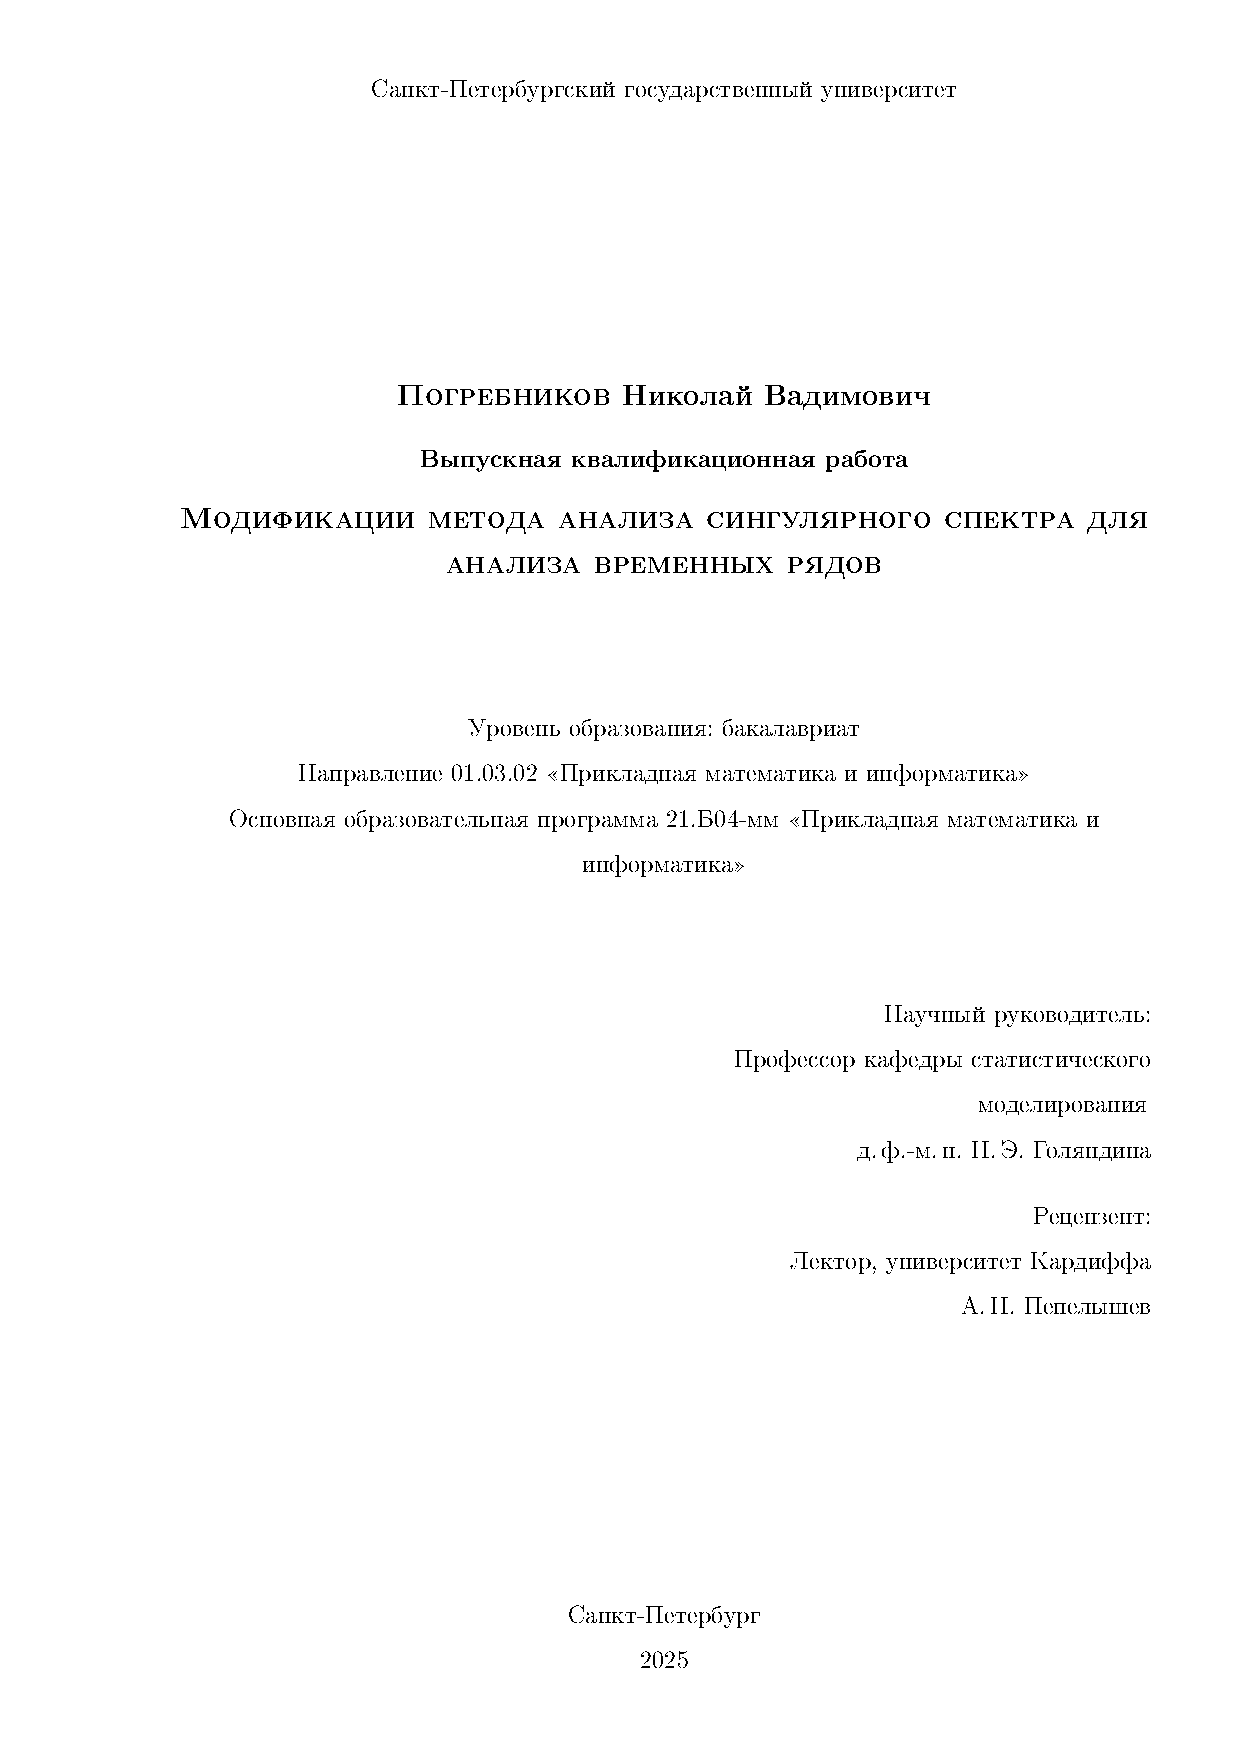
\includepdf[pages=-]{../Title/bachelor.pdf}

\tableofcontents
\noindent
% \textbf{11\textit{} \space Список литературы}

\newpage


\intro


Временные ряды представляют собой упорядоченную последовательность данных, собранных или измеренных в хронологическом порядке. Они играют ключевую роль в анализе и прогнозировании различных явлений в таких областях, как экономика, финансы, климатология и медицина. Понимание эволюции этих явлений во времени критично для выявления тенденций, циклов и аномалий.

Для уточнения терминологии, следует отметить, что \textit{временной ряд} длины \( N \) представляет собой упорядоченную конечную последовательность значений, которая записывается как \( \TS = (x_1, \dots, x_{N}) \), $x_i \in \mathbb{R}$. Одним из основных аспектов анализа временных рядов является разделение их на составляющие. Среди таких компонент важными являются \textit{тренд}, который отражает медленно изменяющуюся долгосрочную динамику ряда, и \textit{сезонность}, представляющая собой периодические колебания, вызванные повторяющимися факторами, такими как климатические или экономические циклы.


В данной работе будут рассмотрены следующие постановки задачи разделения временных рядов:
\begin{enumerate}
	\item \label{item:freq} Разделение временного ряда на компоненты, соответствующие определенным частотным диапазонам;
	\item \label{item:general} Разделение временного ряда на компоненты без привязки к частотным характеристикам, то есть в их исходном виде.
\end{enumerate}


Анализ сингулярного спектра ($\SSA$ \cite{golyandina2001analysis}) --- метод, целью которого является разложение исходного ряда на сумму небольшого числа интерпретируемых компонент, таких как медленно изменяющаяся тенденция (тренд), колебательные компоненты (сезонность) и шум. Позволяет решать как задачу в формулировке \ref{item:freq}, так и её обобщение, представленное в \ref{item:general}. При этом, базовый алгоритм метода $\SSA$ не требует стационарности ряда, знания модели тренда, а также сведений о наличии в ряде периодиках, а за счет своего адаптивного базиса позволяет подстраиваться под любой входной ряд.

В данном исследовании рассматриваются модификации $\SSA$, предложенные другими авторами, а именно: $\GSSA$ \cite{gu2024generalized}, $\CISSA$ \cite{bogalo2020} и $\FSSA$ \cite{haghbin2019functionalsingularspectrumanalysis}.


$\GSSA$ отличается от базового $\SSA$ тем, что он добавляет веса на определенном этапе алгоритма $\SSA$. В разделении компонент между собой это может оказаться полезным, однако также может повлиять на разделимость сигнала от шума в худшую сторону.
Это исследование раскрывает смысловую ценность $\GSSA$ с точки зрения линейных фильтров и отмечает ситуации, где такой алгоритм предпочтительнее стандартного $\SSA$.


В алгоритме $\CISSA$ предложено решение задачи разделения временного ряда компонентам, отвечающим за заранее известные диапазоны частот (задача в постановке \ref{item:freq}). За счет этого можно автоматически группировать компоненты по частотам, однако именно поэтому алгоритм лишается адаптивности, которая имеется в $\SSA$.

$\FSSA$ рассматривается как многомерная модификация $\SSA$, основанная на скрещивании подходов функционального анализа и теории $\SSA$.

Целью работы является описание модификаций в контексте теории $\SSA$ и на этой основе сравнение методов по теоретическим свойствам и численно.


% Для эффективного анализа и понимания структуры временных рядов разработаны различные методы, позволяющие разделить ряд на его компоненты. 
Существует два вида разделимости: \textit{точная разделимость}, которая характеризует способность метода точно выделять отдельные компоненты ряда, и \textit{асимптотическая разделимость}, которая показывает, что ошибка разделения уменьшается с получением новых данных.

Теперь формально. Пусть временной ряд состоит из двух компонент:
\( \TS_N = \TS^{(1)}_N + \TS^{(2)}_N \).
$\mathrm M$ -- метод разделения ряда на компоненты с параметрами $\Theta$.
$\hat{\TS}_N^{(1)}$ -- оценка $\TS_N^{(1)}$.
% , восстановленная $\mathrm M$.
\begin{definition}
	\label{def:exact}
	Ряды \( \TS^{(1)}_N \) и \( \TS^{(2)}_N \) точно разделимы методом $\mathrm M$, если существует такое \( {\Theta} \), что \( \mathrm{MSE}\left(\TS^{(1)}_N, \hat{\TS}^{(1)}_N\right) = 0 \).
\end{definition}

\begin{definition}
	\label{def:asymp}
	Ряды \( \TS^{(1)}_N \) и \( \TS^{(2)}_N \) асимптотически разделимы методом $\mathrm M$, если существует последовательность \( {\Theta}(N)\), \( N \rightarrow \infty \), что \( \mathrm{MSE}\left(\TS^{(1)}_N, \hat{\TS}^{(1)}_N\right) \rightarrow 0 \).
\end{definition}

\begin{comment}
$\hat \TS^{(2)} = \TS - \hat \TS^{(1)}$ является оценкой для $\TS^{(2)}$,
в условиях асимптотической разделимости выполнено
$\mathrm{MSE}\left(\TS^{(2)}, \hat \TS^{(2)}\right) \rightarrow 0$.
\end{comment}

% Методы разделения временных рядов играют ключевую роль в выделении тренда, сезонности и других структурных компонент, что позволяет глубже понять и моделировать временные зависимости.



Далее кратко изложим структуру работы. В главе \ref{sec:ssa} рассматривается базовый метод $\SSA$, его ключевые свойства, а также обобщения на многомерный случай — $\MSSA$ и $\DSSA$.  
Главы \ref{sec:gssa}, \ref{sec:cissa} и \ref{sec:fssa} посвящены алгоритмам $\GSSA$, $\CISSA$ и $\FSSA$ соответственно, где описываются их особенности и отличия от классического подхода.  
В каждом разделе главы \ref{chapter:comparison} проводится теоретическое и численное сравнение модификаций с базовым методом.  
Наконец, в секции \ref{sec:concl} подводятся итоги исследования.


% В секциях \ref{sec:gssa}, \ref{sec:compare_ssa_gssa} показан алгоритм $\GSSA$ и проведено сравнение с $\SSA$. В следующих разделах \ref{sec:cissa}, \ref{sec:comparison_cissa} представлен метод $\CISSA$, также с описанием его основных характеристик и проведено сравнение с $\SSA$. Затем в секциях \ref{sec:fssa}, \ref{sec:compare_fssa_ssa} рассматривается алгоритм $\FSSA$ и его сравнение с $\DSSA$ и $\MSSA$.  В заключительной секции \ref{sec:concl} подведены основные итоги исследования.

\newpage

\chapter{Метод Singular spectrum analysis (SSA)}
\label{sec:ssa}


Рассмотрим базовый метод сингулярного спектрального анализа \cite{golyandina2001analysis}, его свойства, а также многомерные модификации $\MSSA$ и $\DSSA$.

\section{Алгоритм метода SSA}

Фиксируем временной ряд длины $N$: $\TS = (x_1, \dots, x_{N})$, $x_1, \dots, x_{N} \in \mathbb{R}$.

Базовый алгоритм $\SSA$ состоит из четырех шагов.

\subsection*{Вложение}
Параметром этого шага является $L$ --- некоторое целое число (длина окна), $1 < L < N$. Строится $L$-траекторная матрица $\mathbf{X}$, состоящая из $K = N - L + 1$ векторов вложения:
\begin{equation}
	\label{eq:X}
	\EuScript{T} \left(\TS \right) = \EuScript{T}_{SSA} \left(\TS \right)=
	\mathbf{X} =
	\begin{pmatrix}
		x_1    & x_2     & x_3     & \dots  & x_{K}   \\
		x_2    & x_3     & x_4     & \dots  & x_{K+1} \\
		x_3    & x_4     & x_5     & \dots  & x_{K+2} \\
		\vdots & \vdots  & \vdots  & \ddots & \vdots  \\
		x_{L}  & x_{L+1} & x_{L+2} & \dots  & x_{N}
	\end{pmatrix}.
\end{equation}
Полезным свойством является то, что матрица $\mathbf{X}$ имеет одинаковые элементы на антидиагоналях. Таким образом, $L$-траекторная матрица является ганкелевой. $\EuScript{T}_{SSA}$ называется оператором вложения. Обозначим множество всех возможных траекторных матриц как \( \MH \). Буква \( \mathrm{H} \) используется, чтобы подчеркнуть, что эти матрицы имеют ганкелеву структуру.

\subsection*{Сингулярное разложение (SVD)}
Результатом этого шага является сингулярное разложение ($\mathbf{SVD}$) траекторной матрицы ряда.

Пусть $\mathbf{S} = \mathbf{X}\mathbf{X}^{\mathrm{T}}$,
$\lambda_1, \dots, \lambda_L$ --- собственные числа матрицы $\mathbf{S}$, взятые в неубывающем порядке, и
$U_1, \dots, U_L$ --- ортонормированная система собственных векторов, соответствующих собственным числам матрицы $\mathbf S$.

Определим $d = \max{ \{i: \lambda_i > 0 \}}$ и
$V_i = \mathbf{X}^{\mathrm{T}} U_i / \sqrt{\lambda_i}$.
Тогда сингулярным разложением называется представление матрицы в виде:
\begin{equation}
	\mathbf{X} = \mathbf{X}_1 + \dots + \mathbf{X}_d =
	\sum_{i = 1}^{d} \sqrt{\lambda_i} U_i V_{i}^{\mathrm{T}}\label{eq:1}.
\end{equation}

Набор $( \sqrt{\lambda_i}, U_i, V_{i}^{\mathrm{T}})$ называется $i$-й собственной тройкой разложения \eqref{eq:1}.

\subsection*{Группировка}
На основе разложения \eqref{eq:1} производится процедура группировки, которая делит все множество индексов $\{1, \dots, d\}$ на $m$ непересекающихся подмножеств $I_1, \dots, I_m$. Это разбиение является параметром шага группировки.

Пусть $I = \{i_1, \dots, i_p\}$, тогда $\mathbf{X}_I =
	\mathbf{X}_{i_1} + \dots + \mathbf{X}_{i_p}$. Такие матрицы вычисляются для каждого $I = I_1, \dots, I_m$.
В результате получаются матрицы $\mathbf{X}_{I_1}, \dots, \mathbf{X}_{I_m}$. Тем самым разложение \eqref{eq:1} может быть записано в сгруппированном виде:
\begin{equation*}
	\mathbf{X} = \mathbf{X}_{I_1} + \dots + \mathbf{X}_{I_m}.
\end{equation*}

\subsection*{Диагональное усреднение}
Пусть $\mathbf{Y}$ --- матрица размерности $L \times K$. $L^* = \min(L, K), \, K^* = \max(L,K)$. Диагональное усреднение переводит матрицу $\mathbf{Y}$ в временной ряд $g_1, \dots, g_{N} $:

\begin{equation*}
	g_{k}=
	\begin{cases}
		\frac{1}{k+1} \sum\limits_{m=1}^{k+1} y_{m,k-m+2}^{*}           &
		\text{для } 1 \leq k < L^*,                                       \\

		\frac{1}{L^{*}} \sum\limits_{m=1}^{L^*} y_{m,k-m+2}^{*}         &
		\text{для } L^* \leq k < K^*+1 ,                                  \\

		\frac{1}{N-k} \sum\limits_{m=k-K^*+2}^{N-K^*+1} y_{m,k-m+2}^{*} &
		\text{для } K^*+1 \leq k \leq N .                                 \\
	\end{cases}
\end{equation*}


После применения этой операции к матрицам $ \mathbf{X}_{I_1}, \dots, \mathbf{X}_{I_m}$, получаются $m$ новых рядов: $\widetilde{\TS}_1, \dots, \widetilde{\TS}_m$.
Результатом данного шага и всего алгоритма является разложение временного ряда $\TS  = \widetilde{\TS}_1 + \dots + \widetilde{\TS}_m$.

То же самое можно переписать в операторном виде:

\begin{equation*}
	\widetilde{\TS} = \EuScript{T}^{-1} \circ \PH (\widetilde{\TS}^{(k)}),
\end{equation*}

% \begin{equation}
% 	\label{eq:ssa_projector}
% 	(\Pi_{\mathcal{H}}Y)_{ij} = \sum_{(l,k) \in A_s} y_{lk}/w_s,
% \end{equation}

% где \( s = i + j - 1 \), \( A_s = \{(l,k) : l + k = s + 1, 1 \leq l \leq L, 1 \leq k \leq K\} \) и \( w_s = |A_s| \) обозначает количество элементов в множестве \( A_s \). 
$\PH$ -- оператор проектирования на множество $\MH$.


\section{Свойства SSA}


\subsection{Ранг ряда}
\label{subsubsec: ssa_rank}
Зафиксируем ряд $\TS = (x_1, \dots, x_{N})$ длины $N > 3$ и длину окна $L$.

Рассмотрим базовый $\SSA$. В процессе процедуры вложения получаем последовательность векторов вложения:
\begin{equation*}
	\mathrm{X}_i^{(L)} = \mathrm{X}_i = (x_{i-1}, \dots, x_{i+L-2}), \quad i = 1, \dots, K,
\end{equation*}
$\mathcal{L}^{(L)} = \mathcal{L}^{(L)}(\TS) \stackrel{{\rm def}}{{=}} \operatorname{span}(\mathrm X_{1}, \ldots, \mathrm X_{K})$ --- траекторное пространство ряда $\TS$.
При этом, если $\dim \mathcal{L}^{(L)}= \operatorname{rank} \mathbf X = d$, то будем говорить, что ряд $\TS$ имеет $L$-ранг $d$ и записывать это как $\operatorname{rank}_L = d$.

\subsection{Точная разделимость}

Ранее было дано более общее определение \ref{def:exact} точной разделимости. Рассмотрим его с другой стороны.

Пусть временной ряд  $\TS = \TS^{(1)} + \TS^{(2)}$ и задачей является нахождение этих слагаемых. В результате базового алгоритма $\SSA$ при $m = 2$ также получаем $2$ ряда. Возникает вопрос: в каких случаях мы можем так выбрать параметр алгоритма $L$ и так сгруппировать собственные тройки, чтобы получить исходные ряды без смешиваний?
При выборе длины окна $L$ каждый из рядов $\TS^{(1)}$, $\TS^{(2)}$, $\TS$ порождает траекторную матрицу $\mathbf{X}^{(1)}, \mathbf{X}^{(2)}, \mathbf{X}$.

\begin{definition}
	Будем говорить, что ряды $\TS^{(1)}$ и $\TS^{(2)}$ слабо $L$-разделимы, если пространства, порождаемые строками $\mathbf{X}^{(1)}$ и $\mathbf{X}^{(2)}$ ортогональны \cite{golyandina2001analysis}.
\end{definition}

Если выполняется условие слабой $L$-разделимости, тогда существует такое сингулярное разложение траекторной матрицы $\mathbf X$ ряда $\TS$, что его можно разбить на две части, являющиеся сингулярными разложениями траекторных матриц рядов $\TS^{(1)}$ и $\TS^{(2)}$ \cite{golyandina2001analysis}.

\begin{definition}
	Будем говорить, что ряды $\TS^{(1)}$ и $\TS^{(2)}$ сильно $L$-разделимы, если они слабо $L$-разделимы и множества сингулярных чисел траекторных матриц рядов не имеют совпадений \cite{golyandina2001analysis}.
\end{definition}

Если выполняется условие сильной $L$-разделимости, тогда любое сингулярное разложение траекторной матрицы $\mathbf X$ ряда $\TS$ можно разбить на две части, являющиеся сингулярными разложениями траекторных матриц рядов $\TS^{(1)}$ и $ \TS^{(2)}$ \cite{golyandina2001analysis}. Это будет означать, что для разложения ряда базовым методом $\SSA$ с $m = 2$ и таким $L$ будет выполняться
\( \mathrm{MSE}\left(\TS^{(1)}, \hat{\TS}^{(1)}\right) = 0 \) (а значит и \( \mathrm{MSE}\left(\TS^{(2)}, \hat{\TS}^{(2)}\right) = 0 \)).


Рассмотрим таблицу, в которой знаком + отмечены пары рядов, для которых существуют группировка и параметр $L$, при которых они разделимы (точно разделимы). Данная таблица \ref{tab:1} и условия разделимости с доказательствами взяты из книги \cite{golyandina2001analysis}.

\begin{table}[H]
	\begin{center}
		\caption{Точная разделимость.}
		\label{tab:1}
		\scalebox{1}{
			\begin{tabular}{c|ccccc}
				\hline
				        & const & cos & exp & exp cos & ak+b \\ \hline
				const   & -     & +   & -   & -       & -    \\
				cos     & +     & +   & -   & -       & -    \\
				exp     & -     & -   & -   & +       & -    \\
				exp cos & -     & -   & +   & +       & -    \\
				ak+b    & -     & -   & -   & -       & -    \\ \hline
			\end{tabular}}
	\end{center}
\end{table}

Отметим, что $+$ в таблице \ref{tab:1} для $x^{(\cos_1)}_{n} = A_1 \cos\left(2 \pi{\omega_1} n + \varphi_1\right)$,
$x^{(\cos_2)}_{n} = A_2 \cos\left(2 \pi{\omega_2} n + \varphi_2\right)$ достигается, если $L\omega_1 \in \mathbb{N}, \, K\omega_1 \in \mathbb{N}$ или $L\omega_2 \in \mathbb{N}, \, K\omega_2 \in \mathbb{N}$, $\omega_1 \not = \omega_2$ \cite{golyandina2001analysis}.

Однако, по таблице \ref{tab:1} видно, что условия точной разделимости достаточно жесткие и вряд ли выполнимы в реальных задачах. Тогда появляется такое понятие, как асимптотическая разделимость.

\subsection{Асимптотическая разделимость}

Для любого ряда $\TS$ длины $N$ определим
$\TS_{i,j}\,=\,(x_{i-1},\cdot\cdot\cdot,x_{j-1}),\;\;1\,\leq\,i\,\leq\,j\,<\,N.$
Пусть $\TS^{(1)}=(x_{0}^{(1)}, \ldots, x_{N-1}^{(1)})$ и $ \TS^{(2)}=(x_{0}^{(2)}, \ldots,x_{N-1}^{(2)}).$ Тогда определим коэффициент корреляции следующим образом:

% $\EuScript{T}$

\begin{equation*}
	\rho_{i,j}^{(M)}=\frac{\left(\TS_{i,i+M-1}^{(1)},\TS_{j,j+M-1}^{(2)}\right)}{\left|\left|\TS_{i,i+M-1}^{(1)}\right|\right|\left|\left|\TS_{j,j+M-1}^{(2)}\right|\right|}.
\end{equation*}

\begin{definition}[\cite{golyandina2001analysis}]
	Ряды $\TS^{(1)}, \TS^{(2)}$ называются $\varepsilon$-разделимыми при длине окна $L$, если
	\begin{equation*}
		\rho^{(L,K)}\ {\stackrel{\mathrm{def}}{=}}\ \mathrm{max}\left(\operatorname*{max}_{1\leq i,j\leq K}|\rho_{i,j}^{(L)}|,\operatorname*{max}_{1\leq i,j\leq L}|\rho_{i,j}^{(K)}|\right)<\varepsilon
		\text{.}
	\end{equation*}

\end{definition}

\begin{definition}[\cite{golyandina2001analysis}]
	Если $\rho^{(L(N),K(N))} \rightarrow 0$ при некоторой последовательности $L = L(N) $, $N \rightarrow \infty$, то ряды $\TS^{(1)}, \TS^{(2)}$ называются асимптотически $L(N)$-разделимыми .
\end{definition}

Как можно заметить по таблице \ref{tab:2}, для гораздо большего класса функций асимптотическая разделимость имеет место \cite{golyandina2001analysis}.
\begin{table}[H]
	\begin{center}
		\caption{Асимптотическая разделимость.}
		\label{tab:2}
		\scalebox{1}{
			\begin{tabular}{c|ccccc}
				\hline
				        & const & cos & exp & exp cos & ak+b \\ \hline
				const   & -     & +   & +   & +       & -    \\
				cos     & +     & +   & +   & +       & +    \\
				exp     & +     & +   & +   & +       & +    \\
				exp cos & +     & +   & +   & +       & +    \\
				ak+b    & -     & +   & +   & +       & -    \\ \hline
			\end{tabular}}
	\end{center}
\end{table}


\subsection{Частотная разделимость}
\label{subsec:freq_razd}

Следуя \cite[Глава~1, Раздел~1.4]{golyandina2001analysis}, опишем понятие разделимости на основе частот.

Для начала введем определение разложения Фурье.
Пусть $\TS = (x_1, \dots, x_N)$ — временной ряд
\begin{definition}
	Разложение
	\begin{equation}
		\label{eq:fourier}
		x_n = c_0 + \sum\limits_{k = 1}^{\lfloor \frac{N+1}{2} \rfloor}\left(c_k \cos(2\pi n k / N) + s_k \sin(2\pi n k / N) \right),
	\end{equation}
	где $1 \leq n \leq N$ и $s_{N/2} = 0 $ для четного N, называется разложением Фурье ряда $\TS$.
\end{definition}

Таким образом, можно выделить компоненту ряда, отвечающую за частоту $w_k = \frac{k-1}{L}$, $k = 1:\lfloor \frac{N+1}{2} \rfloor$.


Теперь на основе \eqref{eq:fourier} введем понятие периодограммы   как объекта, характеризующего вклад частот в разложение Фурье ряда.

\begin{definition}
	Периодограммой ряда $\TS = (x_1, \dots, x_N)$
	будем называть функцию \(\Pi_f^N\), которая задана на множестве частот
	\(\{k/N, k = 0, \ldots, [N/2]\}\) формулой

	\[
		\Pi_f^N(k/N) = \frac{N}{2}
		\begin{cases}
			2c_0^2        & \text{для } k = 0,       \\
			c_k^2 + s_k^2 & \text{для } 0 < k < N/2, \\
			2c_{N/2}^2    & \text{для } k = N/2.
		\end{cases}
	\]

	Последний случай имеет место только при четном \(N\).
\end{definition}

Фактически, $\Pi_f^N(k/N)$ показывает мощность частоты $\omega_k = \frac{k}{N}$.

\begin{definition}
	$\Pi_f^N(k/N)$ называется мощностью частоты $\omega_k = \frac{k}{N}$. Набор частот $\omega_k$ с положительными мощностями называется носителем периодограммы. Если носитель периодограммы принадлежит некоторому интервалу $\left[a, b\right]$, о этот интервал будем называть диапазоном частот периодограммы.
\end{definition}


Теперь можно перейти к разделимости двух рядов с точки зрения периодограмм.
Пусть $\TS_N = \TS_N^{(1)} + \TS_N^{(2)}$ -- временной ряд длины $N$, $L$ -- длина окна, $K = N-L + 1$.

\begin{proposition}[{\cite[Глава~1, Раздел~1.4]{golyandina2001analysis}}]
	\label{prop:tochn_razd}
	Если носители периодограмм отрезков ряда \( \TS_N^{(1)} \) длины \( L \) не пересекаются с носителями периодограмм отрезков ряда \( \TS_N^{(2)} \) длины \( L \) и аналогичное утверждение справедливо для отрезков рядов длины \( K \), то ряды \( \TS_N^{(1)} \) и \( \TS_N^{(2)} \) слабо разделимы.
\end{proposition}

Теперь можно перейти к аналогичному предложению для асимптотической разделимости. Но для начала определим меру спектральной ортогональности рядов $\TS_N^{(1)}$ и $\TS_N^{(2)}$.

\begin{definition}
	Величину

\[
\rho_{12}^{(\Pi)} {=} \frac{ \sum_{k=0}^{[N/2]} \sqrt{\Pi_{f_1}^N (k/N) \Pi_{f_2}^N (k/N)}}{\sqrt{\sum_{k=0}^{[N/2]} \Pi_{f_1}^N (k/N)} \sqrt{\sum_{k=0}^{[N/2]} \Pi_{f_2}^N (k/N)}} \tag{13}
\]

будем называть \emph{спектральным коэффициентом корреляции} рядов \( \TS_N^{(1)} \) и \( \TS_N^{(2)} \).
\end{definition}

\begin{proposition}[{\cite[Глава~1, Раздел~1.4]{golyandina2001analysis}}]
	\label{prop:ass_razd}
	Если спектральные коэффициенты корреляции отрезков ряда \( \TS^{(1)} \) длины \( L = L(N) \) и отрезков ряда \( \TS^{(2)} \) длины \( L \) равномерно стремятся к нулю при \( N \to \infty \) и аналогичное утверждение справедливо для отрезков рядов длины \( K = K(N) \), то ряды \( \TS^{(1)} \) и \( \TS^{(2)} \) асимптотически разделимы.
\end{proposition}



\subsection{Вложенные варианты SSA}
\label{sec:eossa_and_autogroup}

В алгоритме базового $\SSA$ используется SVD-разложение траекторной матрицы. Поскольку оно обладает наилучшими аппроксимационными свойствами среди методов разложения матриц на матрицы меньшего ранга, применение базового $\SSA$ обеспечивает наилучшее разделение сигнала и шума. Однако, как показывают условия точной и асимптотической разделимости, компоненты сигнала удаётся разделить лишь при достаточно строгих требованиях. Поэтому можно рассматривать различные альтернативные алгоритмы, способным разлагать сигнал на компоненты при менее жёстких условиях.
Отсюда возникает идея вложенных вариантов $\SSA$.

\begin{definition}[\cite{Golyandina_2015}]

	Пусть временной ряд состоит из двух компонент сигнала и шума: $\TS = \mathsf{S} + \TS_{\mathrm{Noise}}=
		\mathsf{S}^{(1)} + \mathsf{S}^{(2)} + \TS_{\mathrm{Noise}}$.

	\textbf{Вложенный вариант SSA} — двухэтапный метод:
	\begin{enumerate}
		\item Задается $r$. $\tilde {\mathbf{S}}$ -- сумма первых $r$ слагаемых SVD разложения траекторной матрицы сигнала $\mathbf S$ с помощью базового $\SSA$ .
		\item Применение другого метода к $\tilde{\mathbf{S}}$ для улучшения разделимости: $\tilde{\mathbf{S }} = \tilde{\mathbf{S}}_1 + \tilde{\mathbf{S } }_2$.
	\end{enumerate}
\end{definition}


Таким образом, получается наилучшим образом разделить как сигнал от шума, так и компоненты сигнала между собой.

В данной работе будут использоваться вложенные варианты $\EOSSA$ и $\FOSSA$. Подробнее про них можно почитать в \cite{golyandina2023intelligent}. Кроме того, благодаря ним можно автоматически группировать компоненты в соответствии с заранее заданными частотами.



\subsection{SSA как линейный фильтр}
Разложение временного ряда методом $\SSA$ можно интерпретировать как применение линейных фильтров. Для дальнейшего исследования введем следующие определения.

\begin{definition}
	Рассмотрим бесконечный временной ряд $\TS = (\dots, x_{-1}, x_0, x_1, \dots)$. Линейный конечный фильтр --- это оператор $\Phi$, который преобразует временной ряд $\TS$ в новый по следующему правилу:
	\begin{equation*}
		y_j = \sum \limits_{i = -r_1}^{r_2} h_i x_{j-i}; \quad r_1, r_2 < \infty.
	\end{equation*}
	Набор коэффициентов ${h_i}$ --- импульсная характеристика фильтра.
\end{definition}

Там, где не оговорено обратного, будем называть линейный конечный фильтр просто линейным фильтром.

\begin{definition}
	Передаточная функция линейного фильтра $\Phi$:
	\begin{equation*}
		H_{\Phi}(z) = \sum \limits_{i = -r_1}^{r_2} h_i z^{-i}.
	\end{equation*}
\end{definition}

\begin{definition}
	Амплитудно-частотная характеристика (АЧХ) линейного фильтра $\Phi$:
	\begin{equation*}
		A_{\Phi}(\omega) = \left| H_{\Phi}\left(e^{i2\pi\omega}\right) \right|.
	\end{equation*}
\end{definition}

АЧХ фильтра  — это график или функция, которая показывает, как фильтр изменяет амплитуды (силу) разных частот входного сигнала.

\begin{definition}
	Фазово-частотная характеристика (ФЧХ) линейного фильтра $\Phi$:
	\begin{equation*}
		\phi_{\Phi}(\omega) = \operatorname{Arg}\left(H_{\Phi}\left(e^{i2\pi\omega}\right)\right).
	\end{equation*}
\end{definition}

Посмотрим, как это выглядит для косинуса. Пусть исходный ряд $x_n^{\cos} = \cos{2\pi \omega n}$. Тогда:
\begin{equation*}
	y_j = A_{\Phi}(\omega) \cos\left(2\pi\omega j + \phi_{\Phi}(\omega) \right)
\end{equation*}

Теперь рассмотрим алгоритм $\SSA$ с точки зрения линейных фильтров \cite[Глава~3, Раздел~3.9]{golyandina2020singular}.
Пусть $\TS = (x_1, \dots, x_{N})$ --- временной ряд длины $N$, $K = N - L + 1, \quad L^{*} = \min(L, K)$. Пусть $L$ будет длиной окна, а $(\sqrt{\lambda},\,U,\,V)$ — одной из собственных троек. Определим диагональную матрицу $N \times N$:
$$
	\mathbf{D} = \text{diag}(1, 2, 3, \ldots, L^{*}-1, L^{*}, L^{*}, \ldots, L^{*}, L^{*}-1, \ldots, 2, 1)
$$
и матрицу  $K \times N$
\[
	\mathbf{W} = \begin{pmatrix}
		u_{1}  & u_{2}  & u_{3}  & \cdots & u_{L}  & 0      & \cdots & 0      & 0      & 0      \\
		0      & u_{1}  & u_{2}  & u_{3}  & \cdots & u_{L}  & 0      & \cdots & 0      & 0      \\
		\vdots & 0      & \ddots & \ddots & \ddots & \cdots & \ddots & 0      & \cdots & 0      \\
		0      & \cdots & 0      & u_{1}  & u_{2}  & u_{3}  & \cdots & u_{L}  & 0      & \vdots \\
		0      & 0      & \cdots & 0      & u_{1}  & u_{2}  & u_{3}  & \cdots & u_{L}  & 0      \\
		0      & 0      & 0      & \cdots & 0      & u_{1}  & u_{2}  & u_{3}  & \cdots & u_{L}
	\end{pmatrix}.
\]
Здесь $U = (u_1, \dots, u_L)$ --- собственный вектор матрицы $\mathbf{S}$.
\begin{theorem}[{\cite[Глава~3, Раздел~3.9]{golyandina2020singular}}]
	\label{th:filter_SSA}
	Компонента временного ряда $\widetilde \TS$, восстановленная с использованием собственной тройки $(\sqrt{\lambda},\,U,\,V)$, имеет вид:
	\[
		\widetilde{\TS}^{{\rm T}} = \mathbf{D}^{-1}\mathbf{W}^{{\rm T}}\mathbf{W}\TS^{\rm T}.
	\]
\end{theorem}
% \begin{proof}
% 	Доказательство можно найти в \cite{golyandina2020singular}.
% \end{proof}

Таким образом, для восстановления методом $\SSA$ средних точек (индексы от $L$ до $K$) имеем следующий фильтр:
\begin{equation}
	\label{eq:representation_ssa_as_filter}
	{\widetilde{x}}_{s} = \sum_{j=-(L-1)}^{L-1} \left( \sum_{k=1}^{L-|j|} u_{k} u_{k+|j|} / L \right) x_{s-j}, \quad L \leq s \leq K.
\end{equation}
Похожим образом можно переписать $\SSA$ через линейные фильтры для точек в начале и конце.

\section{Многомерные варианты SSA}

Временные ряды могут быть не только одномерными, но и многомерными, то есть представлять собой наборы связанных наблюдений.  В данной работе рассматриваются две модификации базового $\SSA$:
$\MSSA$ и $\DSSA$.

Обе эти модификации имеют схожую структуру с одномерным $\SSA$, только нужно переопределить оператор вложения $\EMB$ и понять, какую структуру будет иметь множество траекторных матриц $\MH$.

Таким образом, имеем общую схему алгоритмов $\SSA$:

\begin{enumerate}
	\item \textbf{Вложение}:

	      Для временного ряда $\TS$ строится траекторная матрица:
	      \[
		      \mathbf{X} = \EMB(\TS)
	      \]

	\item \textbf{Разложение}:

	      Траекторная матрица $\mathbf{X}$ разлагается в сумму матриц ранга один:
	      \[
		      \mathbf{X} = \sum_{j=1}^d \mathbf{X}_j
	      \]

	\item \textbf{Группировка}:

	      Элементарные матрицы $\mathbf{X}_j$ разбиваются на группы:
	      \[
		      \mathbf{X} = \mathbf{X}_{I_1} + \cdots + \mathbf{X}_{I_m}, \quad \text{где } \mathbf{X}_{I_k} = \sum_{j \in I_k} \mathbf{X}_j
	      \]

	\item \textbf{Реконструкция}:

	      К сгруппированным матрицам применяется диагональное усреднение:
	      \[
		      \widetilde{\TS} = \widetilde{\TS}_1 + \cdots + \widetilde{\TS}_m, \quad
		      \widetilde{\TS}_k =\EMB^{-1} \circ \PH (\mathbf{X}_{I_k})
	      \]
\end{enumerate}


\subsection{MSSA}
\label{sec:mssa}


% В данной работе рассматриваются две модификации базового $\SSA$:
% $\MSSA$ и $\DSSA$.

Рассмотрим многомерный временной ряд, то есть набор $\{\TS^{(p)} = \left({x^{(p)}_{j}}\right) _{j=1}^{N_p}, \; p = 1, \ldots, s\}$ из $s$ временных рядов длины $N_p$, где $p = 1, \ldots, s$.

Обозначим $\TS = (\TS^{(1)}, \ldots, \TS^{(s)})$ как исходные данные для алгоритма $\MSSA$ \cite{ssa_with_R}. Пусть $L$ -- длина окна, $1 < L < \min(N_p, \; p = 1, \ldots, s)$. Для каждого временного ряда $\TS^{(p)}$ формируем $K_p = N_p - L + 1$ векторов $\mathbf{X}_j^{(p)} = (x_j^{(p)}, \ldots, x_{j+L-1}^{(p)})^T$, где $1 \leq j \leq K_p$. Обозначим $K = \sum_{p=1}^s K_p$. Траекторная матрица многомерного ряда $\TS$ — это матрица размера $L \times K$ следующего вида:

\[
	\EuScript{T}_{\text{MSSA}}(\TS) = \mathbf{X} = [\mathbf{X}_1^{(1)} : \ldots : \mathbf{X}_{K_1}^{(1)} : \ldots : \mathbf{X}_1^{(s)} : \ldots : \mathbf{X}_{K_s}^{(s)}] = [\mathbf{X}^{(1)} : \ldots : \mathbf{X}^{(s)}],
\]

$\mathbf{X}^{(p)} = \EuScript{T}_{\text{SSA}}(\TS^{(p)})$ — траекторная матрица одномерного ряда $\TS^{(p)}$. Таким образом, траекторная матрица системы временных рядов имеет блочно-ганкелеву структуру.
%  Заметим, что

% \[
% 	\EuScript{T}^{-1}_{\text{MSSA}}(\mathbf{X}) = [\EuScript{T}^{-1}_{\text{SSA}}(\mathbf{X}^{(1)}) : \ldots : \EuScript{T}^{-1}_{\text{SSA}}(\mathbf{X}^{(s)})].
% \]



\subsubsection{Комментарии}


Собственные векторы $U_i$ из SVD траекторной матрицы $\mathbf{X} = \sum_i \sqrt{\lambda_i} U_i V_i^{\mathsf{T}}$ формируют общее базисное пространство для всех временных рядов. Векторы $V_i$ содержат подкомпоненты $V_i^{(p)}$, соответствующие каждому ряду:

\begin{equation*}
	V_i = \begin{pmatrix} V_i^{(1)} \\ \vdots \\ V_i^{(s)} \end{pmatrix},
\end{equation*}

$V_i^{(p)} \in \mathbb{R}^{K_p}$ принадлежит строковому пространству $p$-го ряда. $U_i$ отражают общую структуру, $V_i^{(p)}$ — её проявление в отдельных рядах.


Кроме того, преимущество $\MSSA$ проявляется, когда ряды имеют общую с точки зрения $\SSA$ структуру.



\subsection{2d-SSA}

$\DSSA$ -- это расширение базового $\SSA$ для двумерных массивов \cite{ssa_with_R} (например, изображений). Данные представляются в виде матрицы:
\[
	\TS = (x_{ij})_{i,j=1}^{N_x, N_y}, \quad \text{где } N_x \times N_y \text{ — размер массива.}
\]

Матрица содержит наблюдения, упорядоченные по двум пространственным или иным измерениям (например, изображение).

Параметрами метода являются размеры {окна} $(L_x, L_y)$, где $1 \leq L_x \leq N_x$, $1 \leq L_y \leq N_y$.

Определим $\EMB$:

\begin{enumerate}
	\item Из массива $\TS$ выделяются {все возможные подматрицы} размера $L_x \times L_y$ с помощью скользящего окна.
	\item Каждая подматрица $\TS_{k,l}^{(L_x, L_y)}$ преобразуется в столбец: $\mathbf{X}_{k+(l-1)K_x} = \text{vec}(\TS_{k,l}^{(L_x, L_y)})$.
	\item Траекторная матрица строится как объединение этих столбцов:
	      \[
		      \EuScript{T}_{\text{2D-SSA}}(\TS) = \mathbf{X} = [\mathbf{X}_1 : \ldots : \mathbf{X}_{K_x K_y}].
	      \]
\end{enumerate}

Матрица $\mathbf{X}$ имеет {блочно-ганкелеву структуру}:
\[
	\mathbf{X} =
	\begin{pmatrix}
		\mathbf{H}_1     & \mathbf{H}_2       & \ldots & \mathbf{H}_{K_y}   \\
		\mathbf{H}_2     & \mathbf{H}_3       & \ldots & \mathbf{H}_{K_y+1} \\
		\vdots           & \vdots             & \ddots & \vdots             \\
		\mathbf{H}_{L_y} & \mathbf{H}_{L_y+1} & \ldots & \mathbf{H}_{N_y}
	\end{pmatrix},
\]
где каждая $\mathbf{H}_j$ — ганкелевская матрица, построенная из столбцов $\TS$.

\subsubsection{Комментарии}

{Связь с $\MSSA$:} если $L_x = 1$ или $L_y = 1$, $\DSSA$ эквивалентен $\MSSA$ для временных рядов одинаковой длины. Поэтому его можно назвать обобщением $\MSSA$.

Также при применении $\DSSA$ важен порядок следования строк и столбцов в $\TS$, иными словами, предполагается регулярное поведение, как по строкам, так и по столбцам. В отличие от $\MSSA$, где регулярное поведение нужно только по времени.



\newpage




\chapter{Метод Generalized singular spectrum analysis (GSSA)}
\label{sec:gssa}

В этом разделе описана модификация $\SSA$ на основе добавления специальных весов к строкам $L$-траекторной матрицы $\mathbf{X}$ \cite{gu2024generalized}. Это делается для уменьшения растекания частоты (spectral leakage). Авторы метода называют его обобщенным, поскольку базовый $\SSA$ является частным случаем $\GSSA$ с параметром $\alpha = 0$.

\section{Алгоритм метода GSSA}
Алгоритм $\GSSA$ сильно схож с базовым $\SSA$. Фиксируем временной ряд длины $N$: $\TS = (x_1, \dots, x_{N})$, $x_1, \dots, x_{N} \in \mathbb{R}$. Выбирается параметр $\alpha \geq 0$, отвечающий за веса:
\begin{equation*}
	{\boldsymbol{w}}^{(a)} = (w_{1}, w_{2}, \ldots, w_{L}) = \left( \left| \sin\left(\frac{\pi n}{L+1}\right) \right| \right)^\alpha, \quad \text{для } \quad n = 1, 2, \dots, L.
\end{equation*}

\begin{figure}[h]
	\centering
	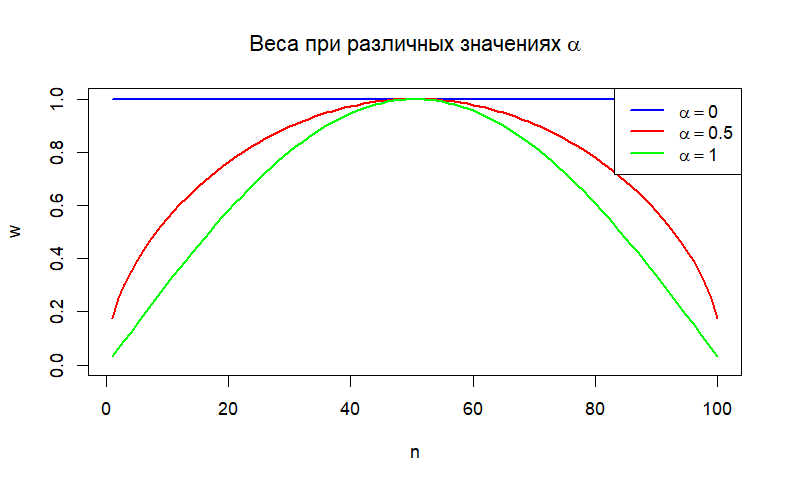
\includegraphics[width=0.8\textwidth]{img/weights.png} % Указываем путь к изображению и ширину
	\caption{График весов для различных значений \(\alpha\).} % Подпись под изображением
	\label{fig:weights} % Метка для ссылки на эту фигуру
\end{figure}


\subsection*{Вложение}
$L$ --- некоторое целое число (длина окна), $1 < L < N$. Строится $L$-траекторная матрица $\mathbf{X}^{(\alpha)}$:
\begin{equation}
	\label{eq:X_alpha}
	\mathbf{X}^{(\alpha)} =
	\begin{pmatrix}
		w_1 x_1   & w_1 x_2     & w_1 x_3     & \dots  & w_1 x_{K}   \\
		w_2 x_2   & w_2 x_3     & w_2 x_4     & \dots  & w_2 x_{K+1} \\
		w_3 x_3   & w_3 x_4     & w_3 x_5     & \dots  & w_3 x_{K+2} \\
		\vdots    & \vdots      & \vdots      & \ddots & \vdots      \\
		w_L x_{L} & w_L x_{L+1} & w_L x_{L+2} & \dots  & w_L x_{N}
	\end{pmatrix}.
\end{equation}

\subsection*{Сингулярное разложение (SVD)}
Этот шаг такой же, как и в $\SSA$, только матрица $\mathbf{X}$ заменяется на $\mathbf{X}^{(\alpha)}$. Будем обозначать собственные тройки в этом случае так: $(\sqrt{\lambda^{(\alpha)}},\,U^{(\alpha)},\,V^{(\alpha)})$.

\subsection*{Группировка}
В точности как в $\SSA$. Тем самым, разложение может быть записано в сгруппированном виде:
\begin{equation*}
	\mathbf{X}^{(\alpha)} = \mathbf{X}^{(\alpha)}_{I_1} + \dots + \mathbf{X}^{(\alpha)}_{I_m}.
\end{equation*}

\subsection*{Взвешенное диагональное усреднение}
Поскольку траекторная матрица была изменена весами, то диагональное усреднение тоже будет зависеть от весов.

Пусть $\mathbf{Y}$ --- матрица размерности $L \times K$. Взвешенное диагональное усреднение переводит матрицу $\mathbf{Y}$ в временной ряд $g_1, \dots, g_{N} $:

\begin{equation*}
	g_{k}=
	\begin{cases}
		\frac{1}{\sum_{n = 1}^k w_n} \sum\limits_{m=1}^{k+1} y_{m,k-m+2}^{*}           &
		\text{для } 1 \leq k < L,                                                        \\

		\frac{1}{\sum_{n = 1}^L w_n} \sum\limits_{m=1}^{L} y_{m,k-m+2}^{*}             &
		\text{для } L \leq k < K+1 ,                                                     \\

		\frac{1}{\sum_{n = k-K+1}^L w_n} \sum\limits_{m=k-K+2}^{N-K+1} y_{m,k-m+2}^{*} &
		\text{для } K+1 \leq k \leq N .                                                  \\
	\end{cases}
\end{equation*}
Применяя данную операцию к матрицам $\mathbf{X}_{I_1}^{(\alpha)}, \dots, \mathbf{X}_{I_m}^{(\alpha)}$, получаются $m$ новых рядов: $\TS^{(\alpha)}_1, \dots, \TS^{(\alpha)}_m$.
Результатом данного шага и всего алгоритма является разложение временного ряда $\TS^{(\alpha)}_1 + \dots + \TS^{(\alpha)}_m = \TS^{(\alpha)}$.



\section{Свойства GSSA}

\subsection{Веса}

Для минимизации эффекта спектрального размывания (spectral leakage), связанного с конечностью временного интервала наблюдений, к исходному ряду применялось оконное преобразование (tapering \cite{weisstein2002crc}). В качестве оконной функции используются степенные синус-косинусные веса (power-of-sine/cosine window).

Данное преобразование выполняет две ключевые функции:
\begin{enumerate}
	\item Снижение краевых эффектов: умножение исходного ряда на убывающую к краям функцию \( w(t) \);
	\item Сглаживание периодограммы: веса используются для усреднения значений.
\end{enumerate}

Такой подход позволяет более точно отделять компоненты ряда друг от друга.


\subsection{Ранг ряда}
Зафиксируем ряд $\TS = (x_1, \dots, x_{N})$ длины $N > 3$ и длину окна $L$.

%Рассмотрим базовый $\SSA$. В процессе процедуры вложения получаем последовательность векторов вложения:
%\begin{equation*}
%	\mathrm{X}_i^{(L)} = \mathrm{X}_i = (x_{i-1}, \dots, x_{i+L-2}), \quad i = 1, \dots, K,
%\end{equation*}
%$\mathcal{L}^{(L)} = \mathcal{L}^{(L)}(\TS) \stackrel{{\rm def}}{{=}} \operatorname{span}(\mathrm X_{1}, \ldots, \mathrm X_{K})$ --- траекторное пространство ряда $\TS$. 
%При этом, если $\dim \mathcal{L}^{(L)}= \operatorname{rank} \mathbf X = d$, то будем говорить, что ряд $\TS$ имеет $L$-ранг $d$ и записывать это как $\operatorname{rank}_L = d$.

В секции \ref{subsubsec: ssa_rank} было введено понятие ранга ряда для базового $\SSA$.
Теперь рассмотрим $\GSSA$ и поймем, что для того же ряда $\operatorname{rank} \mathbf{X}^{(\alpha)} = \operatorname{rank} \mathbf{X}$, а значит, что для $\GSSA$ также применимы понятия $L$-ранга ряда. Из вида \eqref{eq:X_alpha} $\mathbf{X}^{(\alpha)}$ можно получить, что $\mathbf{X}^{(\alpha)} = \operatorname{diag}\left(w_1, w_2, \dots, w_L \right) \mathbf{X} = \operatorname{diag}\left({\boldsymbol{w}}^{(a)}\right) \mathbf{X}$. Поскольку матрица $\operatorname{diag}\left({\boldsymbol{w}}^{(a)}\right)$ имеет ранг равный $L$, она диагональна, то и $\operatorname{rank} \mathbf{X}^{(\alpha)} = \operatorname{rank} \operatorname{diag}\left({\boldsymbol{w}}^{(a)}\right)\mathbf{X} = \operatorname{rank} \mathbf{X}$.

\subsection{GSSA как линейный фильтр}
Аналогично $\SSA$, метод $\GSSA$ можно переписать с помощью линейных фильтров.
Пусть $\TS = (x_1, \dots, x_{N})$ --- временной ряд длины $N$, $K = N - L + 1, \quad L^{*} = \min(L, K)$. $(\sqrt{\lambda^{(\alpha)}},\,U^{(\alpha)},\,V^{(\alpha)})$ -- одна из собственных троек. Определим диагональную матрицу $N \times N$:
$$
	\mathbf{D}^{(\alpha)} = \text{diag}(w_1, w_1 + w_2, \ldots,
	\sum \limits_{i = 1}^{L^*-1}w_i,
	\sum \limits_{i = 1}^{L^*}w_i, \sum \limits_{i = 1}^{L^*}w_i, \ldots, \sum \limits_{i = 1}^{L^*}w_i,
	\sum \limits_{i = 2}^{L^*}w_i, \ldots, w_{L^*-1}+ w_{L^*}, w_{L^*})
$$
и две матрицы  $K \times N$:
\[
	\mathbf{W}^{(\alpha)} = \begin{pmatrix}
		u_{1}^{(\alpha)} & u_{2}^{(\alpha)} & u_{3}^{(\alpha)} & \cdots           & u_{L}^{(\alpha)} & 0                & \cdots           & 0                & 0                & 0                \\
		0                & u_{1}^{(\alpha)} & u_{2}^{(\alpha)} & u_{3}^{(\alpha)} & \cdots           & u_{L}^{(\alpha)} & 0                & \cdots           & 0                & 0                \\
		\vdots           & 0                & \ddots           & \ddots           & \ddots           & \cdots           & \ddots           & 0                & \cdots           & 0                \\
		0                & \cdots           & 0                & u_{1}^{(\alpha)} & u_{2}^{(\alpha)} & u_{3}^{(\alpha)} & \cdots           & u_{L}^{(\alpha)} & 0                & \vdots           \\
		0                & 0                & \cdots           & 0                & u_{1}^{(\alpha)} & u_{2}^{(\alpha)} & u_{3}^{(\alpha)} & \cdots           & u_{L}^{(\alpha)} & 0                \\
		0                & 0                & 0                & \cdots           & 0                & u_{1}^{(\alpha)} & u_{2}^{(\alpha)} & u_{3}^{(\alpha)} & \cdots           & u_{L}^{(\alpha)}
	\end{pmatrix},
\]
\[
	\mathbf{W}_{\boldsymbol{w}}^{(\alpha)} = \begin{pmatrix}
		w_1 u_{1}^{(\alpha)} & w_2 u_{2}^{(\alpha)} & w_3 u_{3}^{(\alpha)} & \cdots               & w_L u_{L}^{(\alpha)} & 0                    & \cdots               & 0                    & 0                    & 0                    \\
		0                    & w_1 u_{1}^{(\alpha)} & w_2 u_{2}^{(\alpha)} & w_3 u_{3}^{(\alpha)} & \cdots               & w_L u_{L}^{(\alpha)} & 0                    & \cdots               & 0                    & 0                    \\
		\vdots               & 0                    & \ddots               & \ddots               & \ddots               & \cdots               & \ddots               & 0                    & \cdots               & 0                    \\
		0                    & \cdots               & 0                    & w_1 u_{1}^{(\alpha)} & w_2 u_{2}^{(\alpha)} & w_3 u_{3}^{(\alpha)} & \cdots               & w_L u_{L}^{(\alpha)} & 0                    & \vdots               \\
		0                    & 0                    & \cdots               & 0                    & w_1 u_{1}^{(\alpha)} & w_2 u_{2}^{(\alpha)} & w_3 u_{3}^{(\alpha)} & \cdots               & w_L u_{L}^{(\alpha)} & 0                    \\
		0                    & 0                    & 0                    & \cdots               & 0                    & w_1 u_{1}^{(\alpha)} & w_2 u_{2}^{(\alpha)} & w_3 u_{3}^{(\alpha)} & \cdots               & w_L u_{L}^{(\alpha)}
	\end{pmatrix}.
\]
Здесь $U = (u_1, \dots, u_L)$ --- собственный вектор матрицы $\mathbf{S}$.
\begin{theorem}
	\label{th:filter_GSSA}
	Компонента временного ряда $\widetilde \TS$, восстановленная с использованием собственной тройки $(\sqrt{\lambda^{(\alpha)}},\,U^{(\alpha)},\,V^{(\alpha)})$, имеет вид:
	\[
		\widetilde{\TS}^{{\rm T}} = {\mathbf{D}^{(\alpha)}}^{-1}
			{\mathbf{W}^{(\alpha)}}^{{\rm T}}
		\mathbf{W}_{\boldsymbol{w}}^{(\alpha)}
		\TS^{\rm T}.
	\]
\end{theorem}
\begin{proof}
	Доказательство проводится аналогично доказательству теоремы $\ref{th:filter_SSA}$.
\end{proof}

Таким образом, для восстановления методом $\GSSA$ средних точек (индексы от $L$ до $K$) имеем следующий фильтр:
\begin{equation}
	\label{eq:representation_gssa_as_filter}
	{\widetilde{x}}_{s} = \sum_{j=-(L-1)}^{L-1} \left( \sum_{k=1}^{L-|j|} u_{k}^{(\alpha)} u_{k+|j|}^{(\alpha)} w_k / \sum\limits_{i = 1}^{L}w_i \right) x_{s-j}, \quad L \leq s \leq K.
\end{equation}
Похожим образом можно переписать $\GSSA$ через линейные фильтры для точек в начале и конце (то представление можно взять из матричной записи в теореме \ref{th:filter_GSSA}).


\newpage






\chapter{Метод Circulant singular spectrum analysis (CiSSA)}
\label{sec:cissa}

%* Переформулировка начала секции 3 из статьи про $\CISSA$ от третьего лица (сказать зачем он создавался, т.е. для автоматического выделения частот)

В этом разделе описана модификация $\SSA$ на основе циркулярной матрицы \cite{bogalo2020}. В отличие от базового $\SSA$, в $\CISSA$ для каждого конкретного $L$ базис разложения остается одинаковым для любого входного временного ряда. Поскольку из-за этого повышается интерпретируемость каждой компоненты в разложении, авторы метода назвали $\CISSA$ автоматизированной версией $\SSA$  в том смысле, что компоненты ряда группируются по частотам самим алгоритмом. Сначала будет рассмотрен метод только для стационарного случая, затем показана применимость модифицированной версии $\CISSA$ при использовании нестационарного ряда.

Стационарность подразумевает неизменность определенных свойств ряда во времени. Определим это понятие формально \cite{golyandina2001analysis}.
\begin{definition}
	Пусть $\TS = (x_1, \dots, x_n, \dots)$ — временной ряд. Ряд $\TS$ называется стационарным, если существует функция $R_{\TS}(k)$ ($-\infty < k < +\infty$) такая, что для любых $k, l \geq 1$
	\begin{equation}
		R_{\TS}^{(N)}(k, l) \overset{\mathrm{def}}{=} \frac{1}{N} \sum_{m=1}^{N} x_{k+m} x_{l+m} \xrightarrow{N \to \infty} R_{\TS}(k - l). \label{eq:R}
	\end{equation}

	Если \eqref{eq:R} выполняется, тогда $R_{\TS}$ называется ковариационной функцией стационарного ряда $\TS$.
\end{definition}

\begin{theorem}[{\cite{golyandina2001analysis}}]
	Пусть $R_{\TS}$ — ковариационная функция стационарного ряда $\TS$. Тогда существует конечная мера $m_{\TS}$, определенная на борелевских подмножествах $(-1/2, 1/2]$, такая, что
	\[
		R_{\TS}(k) = \int_{(-\frac{1}{2}, \frac{1}{2}]} e^{i 2 \pi k \omega} m_{\TS}(d\omega).
	\]


	Мера $m_{\TS}$ называется спектральной мерой ряда $\TS$.
\end{theorem}
% \begin{proof}
% 	Доказательство в \cite{golyandina2001analysis}.
% \end{proof}

%\begin{definition}
%	 ряд $\TS = (x_1, x_2, x_3, \dots)$ называется стационарным, если:
%	\begin{enumerate}
%		\item $\mathrm E (x_t) \equiv \mathrm{const}, \, \forall t \in 1:N$;
%		\item $\mathrm{Cov}(x_t, x_{t+h}) \equiv \mathrm{const}$ при фиксированном h.
%	\end{enumerate}
%\end{definition}

\section{Алгоритм метода CiSSA}
%План:
%\begin{enumerate}
%	\item Алгоритм в текстовом виде.
%	\item ??? Алгоритм на псевдокоде.
%	\item Кратко указать, почему он работает (сослаться на доказательства в статье)
%	\item Пояснить, что делать с нестационарными рядами, показать расширение ряда
%	\item Кратко упомянуть, что алгоритм был реализован на языке R, сослаться на код в GitHub.
%\end{enumerate}

Данный алгоритм, как и $\SSA$, состоит из четырех основных шагов.

Зафиксируем стационарный временной ряд $\TS$ состоящий из $N$ элементов и выберем длину окна $L$.
\subsection*{Вложение}
Такой же, как и в $\SSA$. Считаем матрицу $\mathbf{X}$, заданную в \eqref{eq:X}.

\subsection*{Разложение}

Для каждого $k = 1:L$ вычисляются собственные векторы ${U}_{k}$:
\begin{equation}
	\label{eq:U_k}
	{U}_{k}=L^{-1/2}(u_{k,1\cdot}\cdot\cdot\cdot,u_{k,L}), \, \text{где} \,
	u_{k,j}=\exp\left(-\mathrm{i}2\pi(j-1)\frac{k-1}{L}\right),
\end{equation}
$\text{причем} \, U_{k} = U_{L+2-k}^*$,  $U^*$ --- комплексное сопряжение вектора $U$.


\paragraph{Элементарное разложение \newline}

Для каждой частоты $\omega_k = \frac{k-1}{L}$, $k = 1:\lfloor \frac{L+1}{2} \rfloor$, есть два собственных вектора: $U_k$ и $U_{L+2-k}$. За частоту $\omega_0$ отвечает один собственный вектор --- $U_0$. Если же $L$ --- четное, то частоте $\omega_{\frac{L}{2} + 1}$ будет соответствовать один вектор $U_{\frac{L}{2}+1}$.

Следовательно, индексы группируются следующим образом:
\[
B_k = 
\begin{cases}
\{1\}, & \text{если } k = 1, \\
\{k, L + 2 - k\}, & \text{если } 2 \leq k \leq \left\lfloor \frac{L+1}{2} \right\rfloor \text{ и } k \ne \frac{L}{2} + 1, \\
\left\{ \frac{L}{2} + 1 \right\}, & \text{если } k = \frac{L}{2} + 1 \text{ и } L \bmod 2 = 0.
\end{cases}
\]

%Разложение $\mathbf X_{B_k} = \mathbf X_k + \mathbf X_{L+2-k} = U_k U_k^H \mathbf X + U_{L+2-k} U_{L+2-k}^H \mathbf X$, где $U^H$ --- это комплексное сопряжение и транспонирование вектора $U$.

Таким образом, получается элементарная группировка по частотам $\omega_k$:
\[
\mathbf{X}_{B_k} = 
\begin{cases}
U_1 U_1^\mathrm{H} \mathbf{X}, & \text{если } k = 1, \\[5pt]
U_k U_k^\mathrm{H} \mathbf{X} + U_{L+2-k} U_{L+2-k}^\mathrm{H} \mathbf{X}, & \text{если } 2 \leq k \leq \left\lfloor \frac{L+1}{2} \right\rfloor \text{ и } k \ne \frac{L}{2} + 1, \\[5pt]
U_{\frac{L}{2} + 1} U_{\frac{L}{2} + 1}^\mathrm{H} \mathbf{X}, & \text{если } k = \frac{L}{2} + 1 \text{ и } L \bmod 2 = 0.
\end{cases}
\]

где $U^\mathrm{H}$ --- это комплексное сопряжение и транспонирование вектора $U$.

Результатом данного шага будет разложение исходной матрицы $\mathbf X$ в сумму матриц $\mathbf{X}_{B_k}$, отвечающих периодикам с определенными частотами $\omega_k$:
\begin{equation*}
	\mathbf X = \sum\limits_{k=1}^d \mathbf{X}_{B_k} .
\end{equation*}


\subsection*{Группировка}
Такой же шаг, как и в базовом $\SSA$. Однако группировка будет производиться по $m$ непересекающимся диапазонам частот $\Omega_j$, которые находятся в диапазоне от $0$ до $0.5$. То есть,
$\bigsqcup \limits_{j=1}^m \Omega_j =
			      \bigsqcup \limits_{j=1}^m
			      \left[ \omega_j^{(l)}, \omega_j^{(r)} \right] =
			      [0, 0.5]$. $\mathbf X_{\Omega_j} =\sum\limits_{\omega_k \in \Omega_j} \mathbf{X}_{\omega_k}$.

% заданному произвольному количеству непересекающихся диапазонов $I_i = \left[\omega_{\mathrm{i0}}, \omega_{\mathrm{i1}}\right]$, $\omega_{\mathrm{i0}} \leq \omega_{\mathrm{i1}}$ и $0 \leq \omega_{\mathrm{i0}}, \omega_{\mathrm{i1}} \leq 0.5$, строятся матрицы $\mathbf X_{I_i}$, в которые входят суммы $\mathbf X_{B_k}$, отвечающие частотам $\omega_k: \omega_{i0} \leq \omega_k \leq \omega_{i1}$.

\subsection*{Диагональное усреднение}
Такой же шаг, как и в базовом $\SSA$.

\begin{comment}
$U_k$ можно получить по аналогии с $\SSA$.


Определим автоковариации:
\begin{equation*}
	\hat{\gamma}_m = \frac{1}{N-m} \sum \limits_{t = 1}^{N-m}x_t x_{t+m}, \, m = 0:(L-1).
\end{equation*}
На основе $\hat{\gamma}_m$ определим матрицу:
\begin{equation}
	\label{eq:tepl_mat}
	\hat{\gamma}_{L}=\left(\begin{array}{cccc}
			\hat{\gamma}_{0}   & \hat{\gamma}_{1}   & \ldots & \hat{\gamma}_{L-1} \\
			\hat{\gamma}_{1}   & \hat{\gamma}_{2}   & \ldots & \hat{\gamma}_{L-2} \\
			\vdots             & \vdots             & \vdots & \vdots             \\
			\hat{\gamma}_{L-1} & \hat{\gamma}_{L-2} & \hdots & \hat{\gamma}_{0}
		\end{array}\right).
\end{equation}
Данная матрица $L \times L$ называется Теплицевой и используется в методе Toeplitz SSA (подробнее про данный метод можно прочитать в книге \cite{golyandina2001analysis}). На ее основе составим циркулярную матрицу для алгоритма Circulant SSA \cite{bogalo2020}:


\begin{equation}
	\label{eq:circ_mat}
	\hat{\mathrm{C}}_{L}=\left(\begin{array}{cccc}
			\hat c_{0}   & \hat c_{1}   & \ldots & \hat c_{L-1} \\
			\hat c_{1}   & \hat c_{0}   & \ldots & \hat c_{L-2} \\
			\vdots       & \vdots       & \vdots & \vdots       \\
			\hat c_{L-1} & \hat c_{L-2} & \hdots & \hat c_{0}
		\end{array}\right),
\end{equation}
где $\hat c_m = \frac{L-m}{L}\hat{\gamma}_m + \frac{m}{L}\hat{\gamma}_{L-m}, \, m = 0:L-1$.
Собственные числа матрицы $\hat{\mathrm{C}}_{L}$, определенной в \eqref{eq:circ_mat}, задаются по формуле:
\begin{equation*}
	\lambda_{L,k}=\sum_{m=0}^{L-1}\hat c_{m}\exp\left(i 2\pi m\frac{k-1}{L}\right), \, k = 1:L, \, \text{причем} \, \lambda_{L,k} = \lambda_{L,L+2-k},
\end{equation*}
а собственные вектора, связанные с $\lambda_{L, k}$ --- это векторы $U_k$ из \eqref{eq:U_k}.
\end{comment}

\begin{comment}
\label{comm:proector}
$U_k U_k^\mathrm{H} + U_{L+2-k} U_{L+2-k}^\mathrm{H}$ является оператором проектирования на подпространство, которое порождено синусами и косинусами с частотой $\omega_k = \frac{k-1}{L}$.
\end{comment}
% \begin{proof}
% 	Рассмотрим на примере одного вектора-столбца $X_i = \left(x_i, \dots, x_{i+L}\right)^{\mathrm T}$, где $i = 1, \dots, K$. Возьмем для наглядности $i = 1$.
% 	$$
% 		U_k = L^{-\frac{1}{2}}\left(1, e^{-i2\pi \frac{k-1}{L}}, e^{-i2\pi 2\frac{k-1}{L}}, \dots, e^{-i2\pi (L-1)\frac{k-1}{L}}\right)^{\mathrm T},
% 	$$
% 	$$
% 		U_k^H = L^{\frac{1}{2}}\left(1, e^{i2\pi \frac{k-1}{L}}, e^{i2\pi 2\frac{k-1}{L}}, \dots, e^{i2\pi (L-1)\frac{k-1}{L}}\right).
% 	$$
% 	$$
% 		L^{-\frac{1}{2}}c_k = U_k^H X_1 = x_1 + e^{i2\pi \frac{k-1}{L}} x_2 + e^{i2\pi 2\frac{k-1}{L}} x_3 + \dots + e^{i2\pi (L-1)\frac{k-1}{L}} x_L.
% 	$$
% 	$$
% 		X_1^k = c_k U_k = \left(c_k, c_k e^{-i2\pi \frac{k-1}{L}}, c_k e^{-i2\pi 2\frac{k-1}{L}}, \dots, c_k e^{-i2\pi (L-1)\frac{k-1}{L}}\right)^{\mathrm T}.
% 	$$
% 	Таким образом, получилось проектирование на пространство синусов и косинусов, если разложить комплексную экспоненту.
% 	Если брать всю матрицу $\mathbf X$, выйдет $K$ столбцов, спроектированных на данное пространство.
% \end{proof}
\begin{comment}
В разделе \ref{subsec:cissa_fourier} рассмотрена связь между матрицей $\mathbf X_{B_k}$ и разложениями Фурье для векторов вложения.
\end{comment}

% \noindent \textbf{\large{Нестационарный случай}} \newline \newline
\subsection*{Нестационарный случай}
Для применения данного алгоритма на нестационарных временных рядах, авторами предлагается применить процедуру расширения ряда. Как утверждается авторами статьи \cite{bogalo2020}, после расширения, $\CISSA$ можно применить к нестационарному ряду.
Сама процедура расширения ряда $\TS$ производится с использованием авторегрессионной (AR) модели. Эта процедура позволяет предсказать значения временного ряда за его пределами (экстраполяция) как в правом, так и в левом направлениях на заданное число шагов $H$. Таким образом, трендовая (нелинейная) компонента ряда будет выделяться заметно лучше. В ходе работы алгоритм выполняет следующие шаги:
\begin{enumerate}
	\item \textbf{Построение дифференцированного ряда}:
	      Временной ряд $\TS$ сначала преобразуется в дифференцированный ряд $d \TS$, чтобы удалить трендовые компоненты;

	\item \textbf{Определение порядка AR-модели}:
	      Метод определяет порядок $p$ AR-модели как целую часть от деления длины ряда $N$ на 3. Это значение порядка модели $p$ будет использовано для построения авторегрессионной модели на дифференцированном временном ряде;


	\item \textbf{Построение AR-модели}:
	      После этого для дифференцированного ряда вычисляются коэффициенты авторегрессионной модели $A$ с использованием метода Юла-Уокера, основываясь на определенном ранее порядке $p$;

	\item \textbf{Правое расширение ряда}:
	      С помощью AR-модели ряд $d\TS$ прогнозируется на $H$ шагов вправо. Затем возвращается к своему изначальному состоянию путем интегрирования $d\TS$. Получается расширение исходного ряда $\TS$ на $H$ шагов вправо;

	\item \textbf{Левое расширение ряда}:
	      Аналогично предыдущему пункту, ряд прогнозируется на $H$ шагов влево;

	\item \textbf{Возвращение расширенного ряда}:
	      В конце метод возвращает расширенный временной ряд $\TS_{\mathrm{extended}}$, который содержит как левое, так и правое расширение на $H$ шагов от исходного ряда $\TS$.
\end{enumerate}


Таким образом, алгоритм расширения ряда позволяет выполнять предсказания временного ряда по обе стороны от его границ, основываясь на авторегрессионной модели, построенной на дифференцированном ряде, что полезно для выделения тренда.
\begin{figure}[H]
	\centering
	\includegraphics[width=1\textwidth]{img/extended_IP_values.png}
	\caption{Расширение временного ряда IP values. Красным показан настоящий ряд, черным --- его расширение}
	\label{fig:extended_IP_values}
\end{figure}
Однако поскольку мы рассматриваем расширенный ряд, то и периодические компоненты будут строиться по нему. Поэтому в угоду лучшего выделения трендовой составляющей, будет несколько жертвоваться точность разделения периодических компонентов.
\begin{figure}[H]
	\centering
	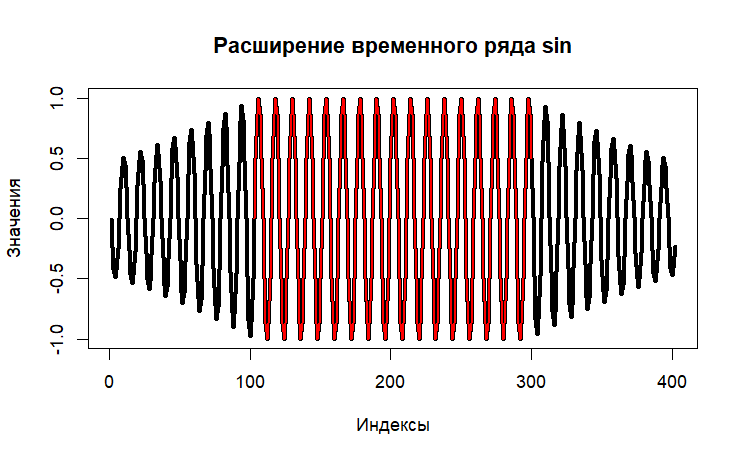
\includegraphics[width=1\textwidth]{img/extended_sin.png}
	\caption{Расширение временного ряда синуса. Красным показан настоящий ряд, черным --- его расширение}
	\label{fig:extended_sin}
\end{figure}

На рисунке \ref{fig:extended_sin} видно, что синус расширился неправильно, от концов настоящего ряда до концов расширенного значения постепенно уменьшались. Как будет показано в секции \ref{sec:comparison_cissa}, это повлияет на значения ошибки выделения сигнала и его компонент.




\section{Свойства}

\subsection{Связь CiSSA с разложением Фурье}
\label{subsec:cissa_fourier}
Для описания конечных, но достаточно длинных рядов можно использовать разложение Фурье. Определение разложения Фурье было дано в \eqref{eq:fourier}.

Алгоритм $\CISSA$ тесно связан с разложением Фурье. По замечанию \ref{comm:proector} видно, что при вычислении $\mathbf X_{B_k} = \mathbf X_k + \mathbf X_{L+2-k} = U_k U_k^\mathrm{H} \mathbf X + U_{L+2-k} U_{L+2-k}^\mathrm{H} \mathbf X$  воспроизводится разложение Фурье для $K$ векторов матрицы $\mathbf{X}$. Затем вычисляется диагональное усреднение $\mathbf X_{B_k}$. А именно, $\CISSA$ можно представить так:
\begin{enumerate}
	\item Вычисляем разложение Фурье для каждого вектора вложения $L$-траекторной матрицы $\mathbf{X}$, состоящей из $K = N - L + 1$ векторов. Получается $K$ разложений Фурье по частотам $\omega_k = \frac{k-1}{L}$, $k = 1:\lfloor \frac{L+1}{2} \rfloor$;
	\item По получившимся разложениям Фурье усредняем значения для соответствующих $x_i$ и частот $\omega_k$.
\end{enumerate}


\subsection{Проблемы фиксированного базиса в CiSSA}
\label{subsec:cissa_fixed_basis_problems}

Одной из особенностей метода $\CISSA$ является использование фиксированного базиса, определенного на пространстве гармоник с частотами, расположенными на регулярной сетке. В отличие от базового $\SSA$, где базис формируется адаптивно в результате сингулярного разложения траекторной матрицы и зависит от структуры входного ряда, $\CISSA$ априори фиксирует частотное представление сигнала. Это принципиальное различие приводит к ряду проблем.

Одна из таких проблем -- растекание спектра. Оно возникает в ситуациях, когда действительная частота сигнальной компоненты не совпадает с узлом частотной решётки $\CISSA$. В таком случае амплитуда истинной частоты оказывается распределённой между несколькими соседними частотами. Это снижает точность восстановления сигнала. Аналогичный эффект наблюдается и при наличии модуляции в частотах, например, когда амплитуда компоненты изменяется во времени. Такие примеры будут рассмотрены в разделе $\ref{sec:comparison_cissa}$.

Для того, чтобы исправить этот недостаток, в $\CISSA$ используется группировка частотных компонент по интервалам $[\omega \pm \delta]$. Однако выбор параметра $\delta$ оказывается сложной задачей и представляет собой компромисс между смещением и дисперсией оценки. Если $\delta$ слишком мало, то компоненту не удаётся полностью захватить, что ведёт к смещению. Если $\delta$ велико, в группу попадает значительное количество шума, что увеличивает дисперсию и приводит к ухудшению оценки.

Таким образом, точность восстановления сигнала в $\CISSA$ зависит от:
\begin{itemize}
  \item ширины интервалов ($\delta$);
  \item наличия модуляции;
  \item расположения частоты сигнальной компоненты относительно частотной решётки базиса.
\end{itemize}

Эти факторы — прямое следствие использования неадаптивного базиса.

Кроме того, на спектральную утечку влияет и выбор окна $L$. При меньших значениях $L$ решётка становится более грубой, что может уменьшить спектральное растекание, но при этом ухудшается способность отделения сигнала от шума. Таким образом, возникает дополнительный компромисс между точностью частотного выделения и устойчивостью к шуму.



\subsection{Точная разделимость}
\label{subsec:cissa_exact}

В разделе \ref{subsec:freq_razd} описана частотная разделимость, являющаяся достаточным условием для точной разделимости базового $\SSA$. Для $\CISSA$ введем точную разделимость также через периодограмму.

\begin{proposition}
	\label{def:exact_cissa}
	Если носители периодограмм отрезков ряда \( \TS_N^{(1)} \) длины \( L \) не пересекаются с носителями периодограмм отрезков ряда \( \TS_N^{(2)} \) длины \( L \), то ряды \( \TS_N^{(1)} \) и \( \TS_N^{(2)} \) точно разделимы методом $\CISSA$ в смысле определения \ref{def:exact}.
\end{proposition}


Предложение \ref{def:exact_cissa} объяснимо тем, что поскольку данный метод является аналогом разложения Фурье, то в смысле сильной разделимости можно точно разделить ряд, в котором одной из компонент является $\cos(2\pi \omega + \varphi)$ с частотой $\omega$ такой, что $L\omega = k \in \mathbb N$, или константа. Для сравнения, при применении базового $\SSA$, условие накладывалось не только на $L\omega \in \mathbb N$, но и на $K\omega \in \mathbb N$.

Поэтому до применения алгоритма необходимо выделить интересующие частоты, то есть знать их заранее, и, исходя из них, выбирать значение $L$.

\subsection{Асимптотическая разделимость}

Аналогично точной разделимости, рассмотрим асимптотическую для $\CISSA$ через периодограмму.

\begin{proposition}
	\label{def:asymp_cissa}
	Если спектральные коэффициенты корреляции отрезков ряда \( \TS^{(1)} \) длины \( L = L(N) \) и отрезков ряда \( \TS^{(2)} \) длины \( L \) равномерно стремятся к нулю при \( N \to \infty \), то ряды \( \TS^{(1)} \) и \( \TS^{(2)} \) асимптотически разделимы методом $\CISSA$ в смысле определения \ref{def:asymp}.
\end{proposition}





\section{Обзор литературы}

% ? Лучше не делать отдельной секцией ? 

В данном разделе рассмотрены применения $\CISSA$ на практике.

\subsection{Cognitive Load Detection through EEG Lead-Wise Feature Optimization and Ensemble Classification}

В статье~\cite{cognitive} рассматриваются несколько наборов данных ЭЭГ под различной нагрузкой, два из которых наиболее значимы:

\begin{itemize}
	\item \textbf{MAT (Mental Arithmetic Task)}: участие студентов в задаче на математический счёт.
	\item \textbf{STEW (Simultaneous Task EEG Workload)}: параллельное выполнение нескольких заданий.
\end{itemize}

Задача исследования заключалась в следующем:

\begin{itemize}
	\item С помощью метода $\CISSA$ (и других различных методов) разлагают исходные сигналы ЭЭГ на несколько компонент, каждая из которых несёт информацию о разных частотных диапазонах и временных структурах.
	\item После разложения из полученных компонент (или их комбинаций) вычисляют числовые признаки: энергетические, энтропийные и другие.
	\item Эти признаки затем подают на вход классификатору (например, $k$NN, SVM или другому алгоритму машинного обучения), чтобы автоматически определить уровень когнитивной нагрузки. Классификация может быть как бинарной (наличие/отсутствие нагрузки), так и многоуровневой (лёгкая/средняя/высокая нагрузка).
\end{itemize}

Таким образом, метод CiSSA был выбран в качестве одного из подходов разложения сигнала по частотам.

Выводом исследования является таблица 5 статьи~\cite{cognitive}, в которой авторы сравнивают по метрикам различные решения задачи. Подходы, связанные с $\CISSA$, являются не самыми наилучшими.



\subsection{Application of visual stratigraphy from line-scan images to constrain chronology and melt features of a firn core from coastal Antarctica}

В работе \cite{Dey_Thamban_Laluraj_Mahalinganathan_Redkar_Kumar_Matsuoka_2023} исследовалось таяние ледников, а также анализировались данные визуальной стратиграфии (VS) для построения хронологии фирнового керна из прибрежной Антарктиды. Основной задачей было отделение долгосрочного тренда, связанного с изменением плотности фирна, от сезонных сигналов, обусловленных включениями пыли и морской соли.

Для разложения сигнала по частотам был выбран алгоритм $\CISSA$. Длина окна $L = 10$, поскольку <<дальнейшее её увеличение не оказывало существенного влияния на результаты>>. Хотя профиль визуальной стратиграфии является функцией глубины, а не времени, последовательность данных вдоль керна интерпретируется как время. Это обусловлено тем, что слои снега и льда откладываются ежегодно, и глубина в этом контексте отражает хронологическую последовательность. Измерения производились с частотой 5 сантиментов по глубине от 0 до 50 метров. Таким образом, методы обработки сигналов, разработанные для временных рядов, включая $\CISSA$, применимы и к профилям по глубине. 


\noindent \textbf{Ключевые этапы анализа}:

\begin{itemize}
	\item \textbf{Первая компонента (RC1)}: отвечала за долгосрочный тренд, связанный с постепенным увеличением плотности фирна с глубиной;
	\item \textbf{Компоненты со второй по пятую (RC2-RC5)}: отражали сезонность, обусловленную изменениями в содержании пыли и морских солей;
	\item \textbf{Остальные компоненты}: содержали шумовой сигнал и не учитывались в дальнейшем анализе.
\end{itemize}

Таким образом, метод $\CISSA$ был использован как инструмент частотного разложения.

\subsection{Выводы}

В рассмотренных работах $\CISSA$ используется как прикладной инструмент для разделения сигнала по частотам. В работе \cite{cognitive} это конкретные частоты, а для \cite{Dey_Thamban_Laluraj_Mahalinganathan_Redkar_Kumar_Matsuoka_2023} это инструмент для выделения тренда. По целям использования алгоритмов, можно сделать вывод, что с таким же успехом можно было применить базовый $\SSA$ с автоматической группировкой по компонентам, как сказано в секции \ref{sec:eossa_and_autogroup}.


\newpage








\chapter{Метод Functional singular spectrum analysis (FSSA)}
\label{sec:fssa}

Functional $\SSA$ -- метод для анализа функциональных временных рядов \cite{haghbin2019functionalsingularspectrumanalysis}. Предлагается объединить теорию многомерного функционального анализа главных компонент (MFPCA) и $\SSA$.

Авторы метода $\FSSA$ сравнивают его с $\MSSA$ и динамическим функциональным анализом главных компонент (dFPCA), показывая преимущество использования $\FSSA$ в разделении компонент функциональных данных, особенно для нестационарных рядов.

В данном разделе преимущественно используются обозначения из статьи \cite{haghbin2019functionalsingularspectrumanalysis} авторов метода. Таким образом, например, $\TS$ заменяется на $\pmb x$.





Рассмотрим, основные определения.
Функциональным временным рядом будем называть ${\pmb x}\in\mathbb{H}^k$: ${\pmb x}(s)=\begin{pmatrix} x_1(s),\ldots,x_N(s)\end{pmatrix}^\top$, $x_i\in\mathbb{H} =\mathcal{L}^2([0,1])$, $s\in[0,1]$. Скалярное произведение: $\langle\pmb x,\pmb y\rangle_{\mathbb{H}^k}=\sum_{i=1}^k\langle x_i,y_i\rangle$, $\langle x,y\rangle=\int_0^1 x(s)y(s)ds$. Также определим тензорное произведение: для $x\in\mathbb{H}_1$, $y\in\mathbb{H}_2$, оператор $x\otimes y:\mathbb{H}_1\to\mathbb{H}_2$, $(x\otimes y)h=\langle x,h\rangle y$, $h\in\mathbb{H}_1$.

% \begin{itemize}
% 	\item \textbf{Функциональный временной ряд:} $\textbf{y}_N=(y_1,\ldots,y_N)^\top$, длина $N$, $y_i:[0,1]\to\mathbb{R}$, $y_i\in\mathbb{H}=\mathcal{L}^2([0,1])$ с $\langle x,y\rangle=\int_0^1 x(s)y(s)ds$.

% 	\item \textbf{Пространство $\mathbb{H}^k$:} Декартово произведение $k$ копий $\mathbb{H}$. \\ Элемент ${\TS}\in\mathbb{H}^k$: ${\TS}(s)=\begin{pmatrix} x_1(s),\ldots,x_k(s)\end{pmatrix}^\top$, $x_i\in\mathbb{H}$, $s\in[0,1]$. Скалярное произведение: $\langle\TS,\pmb y\rangle_{\mathbb{H}^k}=\sum_{i=1}^k\langle x_i,y_i\rangle$.

% 	\item \textbf{Тензорное произведение:} Для $x\in\mathbb{H}_1$, $y\in\mathbb{H}_2$, оператор $x\otimes y:\mathbb{H}_1\to\mathbb{H}_2$, $(x\otimes y)h=\langle x,h\rangle y$, $h\in\mathbb{H}_1$.

% 	\item \textbf{Пространство $\mathbb{H}^{L\times K}$:} Линейное пространство операторов $\mathcal{Z}:\mathbb{R}^K\to\mathbb{H}^L$, заданных $[z_{i,j}]_{i=1,\ldots,L}^{j=1,\ldots,K}$,
% 	      \begin{equation}\label{eq: z operator}
% 		      \mathcal{Z}\pmb{a}=\begin{pmatrix} \sum_{j=1}^K a_j z_{1,j} \\ \vdots \\ \sum_{j=1}^K a_j z_{L,j} \end{pmatrix}, \ z_{i,j}\in\mathbb{H}, \ \pmb{a}=(a_1,\ldots,a_K)\in\mathbb{R}^K.
% 	      \end{equation}

% \end{itemize}






\section{Алгоритм FSSA}
Алгоритм схож по структуре с базовым $\SSA$.

Пусть ${\pmb x}(s)=\begin{pmatrix} x_1(s),\ldots,x_N(s)\end{pmatrix}^\top$ -- функциональный временной ряд длины $N$.
Для целого числа $1\leq L\leq{N}/{2}$ положим $K=N-L+1$ и определим множество многомерных функциональных векторов в $\mathbb{H}^L$ как
\begin{equation}\label{flvec}
	{\pmb x}_j(s):= \begin{pmatrix} y_j(s), y_{j+1}(s), \ldots, y_{j+L-1}(s)\end{pmatrix}^\top,\ \ j=1,\ldots, K,
\end{equation}
где ${\pmb x}_j$ обозначают функциональные векторы. Следующий алгоритм предоставляет результаты $\FSSA$ в четыре этапа.

\subsection*{Вложение}
Траекторный оператор $\mathcal{X}:\mathbb{R}^K \rightarrow \mathbb{H}^L$.
\begin{equation}
	\label{eq:traj}
	\mathcal{X}{\pmb a}:=\sum_{j=1}^K a_j{\pmb x}_j=
	\begin{pmatrix} \sum_{j=1}^K a_jy_j\\ \sum_{j=1}^K a_j y_{j+1}\\ \vdots\\ \sum_{j=1}^K a_j y_{j+L-1} \end{pmatrix},
	\ {\pmb a}=\left(a_1,\ldots, a_K\right)^\top \in\mathbb{R}^K.
\end{equation}

Кроме того, $\mathcal{X}=\EuScript{T}\pmb {x}$, где $\EuScript{T}$ — оператор вложения. Вычисление $\mathcal{X} \pmb{a}$ в заданной точке $s\in [0,1]$ эквивалентно матричному произведению ${\bf X}(s)\pmb{a}$, где ${\bf X}(s)$ — это $L \times K$ ганкелева матрица, заданная как
\begin{equation}\label{ftraj}
	{\bf X}(s)=\begin{bmatrix} {\pmb x}_1(s), \ldots, {\pmb x}_K(s) \end{bmatrix}.
\end{equation}


Оператор $\mathcal{X}$ является ограниченным линейным оператором. Если определить $\mathcal{X}^*:\mathbb{H}^L \rightarrow \mathbb{R}^K$ как
\begin{equation}
	\mathcal{X}^*{\pmb z}=
	\begin{pmatrix} \sum_{i=1}^L \langle y_i, z_i\rangle\\ \sum_{i=1}^L \langle y_{i+1}, z_i\rangle\\ \vdots\\ \sum_{i=1}^L \langle y_{i+K-1}, z_i\rangle \end{pmatrix},
	\ {\pmb z}=\left(z_1,\ldots, z_L\right)^\top\in\mathbb{H}^L,
\end{equation}
то $\mathcal{X}^*$ является сопряжённым оператором для $\mathcal{X}$.

\subsection*{Разложение}
Определим оператор $\mathcal{S}: \mathbb{H}^L\rightarrow \mathbb{H}^L$ как $\mathcal{S}:=\mathcal{X}\mathcal{X}^*$. Следовательно, для заданного ${\pmb z}\in \mathbb{H}^{L}$ это означает, что
\begin{align}\label{eq: s-operator}
	\mathcal{S}{\pmb z} &
	=\sum_{j=1}^K\sum_{i=1}^L \langle y_{i+j-1} , z_i \rangle {\pmb x}_j
	=\sum_{j=1}^K \langle {\pmb x}_j , {\pmb z} \rangle_{\mathbb{H}^L} {\pmb x}_j
	=\sum_{j=1}^K ({\pmb x}_j \otimes {\pmb x}_j) {\pmb z}.
\end{align}


\begin{proposition}[{\cite[Раздел~3.1]{haghbin2019functionalsingularspectrumanalysis}}]
	Существует ортонормированная система базисных векторов $\{\boldsymbol{\psi}_{i},\ i\in\mathbb{N}\}$ в пространстве $\mathbb{H}^{L}$, такая что
\[
\boldsymbol{\mathcal{S}}\boldsymbol{\psi}_{i} = \lambda_{i}\boldsymbol{\psi}_{i}, \quad \text{причём } \lambda_{i} \to 0 \text{ при } i \to \infty.
\]

Кроме того, 
\[
\boldsymbol{\mathcal{S}} = \sum_{i=1}^{\infty} \lambda_{i} \boldsymbol{\psi}_{i} \otimes \boldsymbol{\psi}_{i}.
\]
\end{proposition}


Для любого положительного $i$ определим оператор $\mathcal{X}_i:\mathbb{R}^K\rightarrow\mathbb{H}^L$, заданный как
\begin{equation}\label{eq: elementary oprator}
	\mathcal{X}_i \pmb{a}:=\sum_{j=1}^K a_j (\pmb{\psi}_i\otimes \pmb{\psi}_i){\pmb x}_j= (\pmb{\psi}_i\otimes \pmb{\psi}_i)\sum_{j=1}^K a_j{\pmb x}_j.
\end{equation}

Вычисление $\mathcal{X}_i \pmb{a}$ в заданной точке $s\in [0,1]$ эквивалентно матричному произведению ${\bf X}_i(s)\pmb{a}$, где ${\bf X}_i(s)$ — это $L \times K$ матрица, заданная как
\begin{align}\label{eq:elementary mat}
	{\bf X}_i(s) & :=
	\begin{bmatrix} \langle\pmb{\psi}_i, {\pmb x}_1\rangle_{\mathbb{H}^L} \pmb{\psi}_i(s), \ldots, \langle\pmb{\psi}_i, {\pmb x}_K\rangle_{\mathbb{H}^L} \pmb{\psi}_i(s) \end{bmatrix}
	\notag            \\ &\ =
	\begin{bmatrix} (\pmb{\psi}_i\otimes \pmb{\psi}_i){\pmb x}_1(s), \ldots, (\pmb{\psi}_i\otimes \pmb{\psi}_i){\pmb x}_K(s) \end{bmatrix}.
\end{align}

% Заметим, что ${\bf X}_i(s)$ можно рассматривать как функциональное расширение элементарных матриц, определённых в \eqref{eq: primary}, где ${\bf X}_i(s)$ проецирует столбцы ${\bf X}(s)$ в пространство, порождённое $\pmb{\psi_i}(s)$.


Элементарные операторы $\mathcal{X}_i$ раскладывают траекторный оператор $\mathcal{X}$ как
\begin{equation}\label{eq:elementary operators}
	\mathcal{X}=\sum_{i=1}^\infty \mathcal{X}_i.
\end{equation}

Следующая теорема предоставляет сингулярное разложение (SVD) траекторного оператора $\mathcal{X}$ для получения соответствующих собственных троек ($\sqrt{\lambda_i}, \pmb{v}_i, \pmb{\psi}_i$) на этапе декомпозиции \cite{haghbin2019functionalsingularspectrumanalysis}.
\begin{theorem}
	\label{thm:svd}
	Пусть ${\{\pmb{\psi}_i\}_{i=1}^\infty}$ и ${\{\lambda_i\}_{i=1}^\infty}$ — собственные элементы $\mathcal{S}$, и
	\begin{equation}
		\mathcal{S}^\dag:=\mathcal{X}^*\mathcal{X}=
		\begin{bmatrix}
			\sum_{i=1}^L\langle y_i, y_{i}\rangle       & \cdots & \sum_{i=1}^L\langle y_i, y_{i+K-1}\rangle       \\
			\vdots                                      & \ddots & \vdots                                          \\
			\sum_{i=1}^L\langle y_{i+K-1}, y_{i}\rangle & \cdots & \sum_{i=1}^L\langle y_{i+K-1}, y_{i+K-1}\rangle \\
		\end{bmatrix}.
	\end{equation}
	Тогда сингулярное разложение траекторного оператора $\mathcal{X}$ можно записать как
	\begin{equation}
		\label{eq: svd}
		\mathcal{X} = \sum_{i=1}^\infty \sqrt{\lambda_i}\textbf{v}_i\otimes \pmb{\psi}_i,
	\end{equation}
	где
	$\textbf{v}_i=
		\begin{pmatrix} \frac{\langle\pmb{\psi}_i, {\pmb x}_1\rangle_{\mathbb{H}^L}}{\sqrt{\lambda_i}} , \ldots,\frac{ \langle\pmb{\psi}_i, {\pmb x}_K\rangle_{\mathbb{H}^L}}{\sqrt{\lambda_i}} \end{pmatrix}^\top$. Кроме того, для любого $\pmb{a}\in\mathbb{R}^K$, используя \eqref{eq: svd}, мы имеем
	\begin{equation}
		\mathcal{X}\pmb{a} = \sum_{i=1}^\infty \sqrt{\lambda_i} \langle \textbf{v}_i, \pmb{a}\rangle_{\mathbb{R}^K} \pmb{\psi}_i,
	\end{equation}
	где
	\begin{itemize}
		\item[i)] $\{\lambda_i\}_{i=1}^\infty$ — множество неубывающих собственных значений $\mathcal{S}^\dag$, и
		\item[ii)] $\pmb{v}_i$ — соответствующие ортонормированные собственные векторы $\mathcal{S}^\dag$, удовлетворяющие $\mathcal{X}\pmb{v}_i = \sqrt{\lambda_i} \pmb{\psi}_i$.
	\end{itemize}
\end{theorem}

\subsection*{Группировка}

Аналогично базовому $\SSA$. Получается
\begin{equation}\label{eq:grouping}
	\mathcal{X}=\mathcal{X}_{I_1}+\mathcal{X}_{I_2}+\cdots+\mathcal{X}_{I_m}.
\end{equation}


\subsection*{Диагональное усреднение}

Для заданного $q$ ($1\leq q\leq m$) используется $\EuScript{T}^{-1}$ для преобразования оператора $\mathcal{X}_{I_q}$ из \eqref{eq:grouping} в $\tilde{\pmb x}^q$.

% Поскольку $\mathcal{X}_{I_q}\in\mathbb{H}^{L\times K}$, сначала выполняется проекция на $\mathbb{H}_H^{L\times K}$, замкнутое подпространство $\mathbb{H}^{L\times K}$.

Элементы $\mathcal{X}_{I_q}$ и $\tilde{\mathcal{X}}_{I_q}$ обозначаются $[x_{i,j}^{q}]$ и $[\tilde{x}_{i,j}^{q}]$. Метод диагонального усреднения  обобщается на $\mathbb{H}^{L\times K}$, где
\begin{equation}\label{fdiag-ave}
	\tilde{x}_{i,j}^{q}=\frac{1}{n_s}\sum_{(l,k): l+k=s} x_{l,k}^q,
\end{equation}
$s=i+j$, $n_s$ — число пар $(l,k)$, таких что $l+k=s$. 
% Проекция обозначается $\Pi_\mathbb{H}:\mathbb{H}^{L\times K}\to\mathbb{H}_H^{L\times K}$, и $\tilde{\mathcal{X}}_{I_q}=\Pi_\mathbb{H} \mathcal{X}_{I_q}$.

Как итог: $\tilde{\pmb x}^q=\EuScript{T}^{-1}\tilde{\mathcal{X}}_{I_q}$.


\section{Практическая реализация алгоритма FSSA}

Для использования на практике алгоритма $\FSSA$, нужно понять, как использовать дискретные данные с теорией, основанной на непрерывности по $s$. 

\subsection*{Преобразование}

На вход алгоритму приходят 
дискретные данные \( \{x_j(s_k)\}_{j=1,\dots,N}^{ k = 1, \dots, n} \)  в виде матрицы. После чего они преобразуются в функции \( x_j(s) \in \mathbb{H} \) на \( [0,1] \) с использованием базисного разложения:
\[
	x_j(s) = \sum_{i=1}^d a_{i,j} \nu_i(s),
\]
где \( \{\nu_i\}_{i=1}^d \) — базис (например, B-сплайны), \( d \) является параметром алгоритма. Получается функциональный временной ряд \( \pmb {x} = \{x_1(s), \dots, x_N(s)\} \).



\subsection*{Вложение}
Задаётся \( L\). Формируются векторы:
\[
	\pmb{x}_j(s) = (x_j(s), \dots, x_{j+L-1}(s))^\top, \quad j=1,\dots,K, \quad K=N-L+1.
\]
Траекторный оператор \( \mathcal{X}: \mathbb{R}^K \to \mathbb{H}^L \) представлен матрицей \( \mathbf{X}(s) = [\pmb{x}_1(s), \dots, \pmb{x}_K(s)] \), вычисляемой через базисные коэффициенты \( a_{i,j} \).

\subsection*{Разложение}

Вычисляется оператор \( \mathcal{S} = \mathcal{X} \mathcal{X}^* \), представленный матрицей \( \mathbf{S} \) в базисе \( \mathbb{H}_d^L \). Формируется базис \( \{\mathbf{\phi}_k\}_{k=1}^{Ld} \), где \( \mathbf{\phi}_k \) — вектор с \( \nu_{q_k} \) на позиции \( r_k \), \( k = (q_k-1)L + r_k \). Вычисляются матрицы:
\[
	\mathbf{G} = [\delta_{r_i,r_j} \langle \nu_{q_i}, \nu_{q_j} \rangle]_{i,j=1}^{Ld}, \quad \mathbf{S}_0 = \left[\sum_{m=1}^K \langle x_{r_i+m-1}, \nu_{q_i} \rangle \langle x_{r_j+m-1}, \nu_{q_j} \rangle\right]_{i,j=1}^{Ld}.
\]
\[
	\mathbf{S} = \mathbf{G}^{-1} \mathbf{S}_0.
\]
Находятся собственные значения \( \lambda_i \) и векторы \( \mathbf{c}_{\mathbf{\psi}_i} \) матрицы \( \mathbf{S} \). Собственные функции: \( \mathbf{\psi}_i = \sum_{k=1}^{Ld} (\mathbf{c}_{\mathbf{\psi}_i})_k \mathbf{\phi}_k \). Вычисляются элементарные операторы \( \mathcal{X}_i = (\mathbf{\psi}_i \otimes \mathbf{\psi}_i) \mathcal{X} \).

\subsection*{Группировка}
Аналогично теоретической группировке \eqref{eq:grouping}.
\begin{equation*}
	\mathcal{X}=\mathcal{X}_{I_1}+\mathcal{X}_{I_2}+\cdots+\mathcal{X}_{I_m}.
\end{equation*}

\subsection*{Реконструкция}
Для \( \mathcal{X}_{I_q} \) выполняется диагональное усреднение:
\[
	\tilde{x}_{i,j}^q = \frac{1}{n_s} \sum_{(l,k): l+k=i+j} x_{l,k}^q,
\]
где \( x_{l,k}^q \) — элементы \( \mathcal{X}_{I_q} \), $n_s$ -- количество пар $(l, k)$, равных $i+j$.  Получаем \( \tilde{\mathcal{X}}_{I_q} = \Pi_\mathbb{H} \mathcal{X}_{I_q} \). Затем применяется \( \EuScript{T}^{-1} \): \( \tilde{\pmb{x}}_N^q = \EuScript{T}^{-1} \tilde{\mathcal{X}}_{I_q} \), выраженное через базисные коэффициенты.



% \section{Разделимость}\label{subsec: Separability}

% Рассматривается $\textbf{y}_N=\textbf{y}_N^{(1)}+\textbf{y}_N^{(2)}$, где $\textbf{y}_N^{(i)}=\{y_1^{(i)},\ldots,y_N^{(i)}\}$, $i=1,2$, — функциональные временные ряды (FTS). Для фиксированной длины окна $L$ для каждого ряда $\textbf{y}_N^{(i)}$ обозначается $\{{\pmb x}_{k}^{(i)}\}_{k=1}^K$ — последовательность функциональных сдвинутых векторов, $\mathcal{L}^{(i)}$ — линейное пространство, порождённое $\{{\pmb x}_{k}^{(i)}\}_{k=1}^K$. Разделимость рядов $\textbf{y}_N^{(1)}$ и $\textbf{y}_N^{(2)}$ эквивалентна $\mathcal{L}^{(1)}\bot\mathcal{L}^{(2)}$, то есть $\langle {\pmb x}_{k}^{(1)},{\pmb x}_{k^\prime}^{(2)}\rangle_{\mathbb{H}^L}=0$ для всех $k,k^\prime=1,\ldots,K$.

% Необходимое условие разделимости определяется через w-корреляцию. Взвешенное скалярное произведение рядов $\textbf{y}_N^{(1)}$ и $\textbf{y}_N^{(2)}$ задаётся как
% \begin{equation}\label{winn}
% 	\langle \textbf{y}_N^{(1)},\textbf{y}_N^{(2)}\rangle_w=\sum_{i=1}^N w_i \langle y_i^{(1)},y_i^{(2)}\rangle,
% \end{equation}
% где $w_i=\min\{i,L,N-i+1\}$. Ряды $\textbf{y}_N^{(1)}$ и $\textbf{y}_N^{(2)}$ называются w-ортогональными, если
% \begin{equation}
% 	\langle \textbf{y}_N^{(1)},\textbf{y}_N^{(2)}\rangle_w=0.
% \end{equation}

% \begin{theorem}\label{thm:fSep}
% 	Разделимость рядов $\textbf{y}_N^{(1)}$ и $\textbf{y}_N^{(2)}$ влечёт их w-ортогональность \cite{haghbin2019functionalsingularspectrumanalysis}.
% \end{theorem}



\newpage




\chapter{Сравнения алгоритмов}
\label{chapter:comparison}


\section{Сравнение SSA и GSSA}
\label{sec:compare_ssa_gssa}
В данном разделе сравниваются алгоритмы базового $\SSA$ и $\GSSA$ с параметром $\alpha \not = 0$. Все вычисления, а также код метода $\GSSA$ можно найти в репозитории \cite{spbu_cissa_coursework_github}.


\subsection{Линейные фильтры}
Чтобы понять отличие, рассмотрим методы с точки зрения линейных фильтров: по представлениям \eqref{eq:representation_ssa_as_filter} и \eqref{eq:representation_gssa_as_filter} можно построить амплитудно-частотные характеристики.

Рассмотрим временной ряд \[\TS = \left\{\sin\left(\frac{2\pi}{12}n\right), \, n = 1, \dots, N\right\}, \, N = 96 \cdot 2 - 1, L = 48.\]
Построим АЧХ для первых двух компонент при $\alpha$, равных $0$ (базовый $\SSA$), $\frac{1}{2}$, $1$, $2$.
\begin{figure}[H]
	\centering
	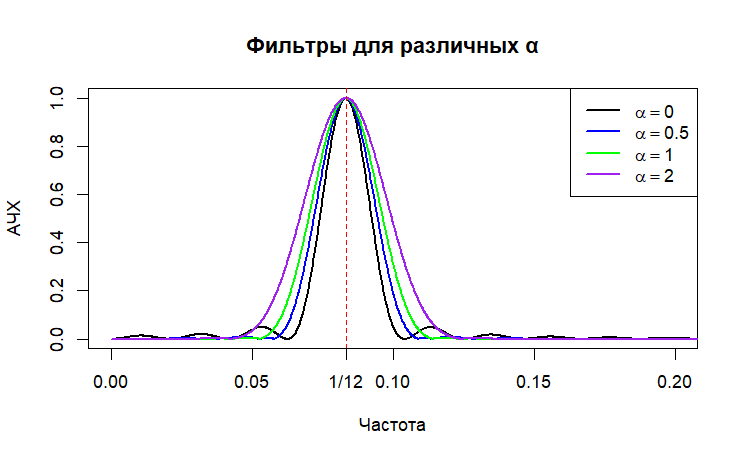
\includegraphics[width=1\textwidth]{img/various_alphas.png}
	\caption{АЧХ фильтров для первых двух компонент SVD ряда $\TS = \left\{\sin\left(\frac{2\pi}{12}n\right), \, n = 1, \dots, N\right\}$ при разных $\alpha$.}
	\label{fig:various_alphas}
\end{figure}
На рисунке \ref{fig:various_alphas} показано, как фильтры ведут себя для различных значений параметра \(\alpha\). Для всех рассмотренных значений \(\alpha\) фильтры подавляют частоты, значительно отличающиеся от частоты синуса $ \omega = \frac{1}{12}$. При малых значениях \(\alpha\), таких как \(\alpha = 0\), наблюдается волнообразное поведение фильтра, что указывает на частичное захватывание соседних частот, хотя и не близких к частоте синуса. С увеличением \(\alpha\) это волнообразное поведение уменьшается, но фильтр начинает захватывает больше частот, близких к \(\frac{1}{12}\).

Таким образом, метод $\GSSA$ должен работать лучше $\SSA$ в случае, когда временной ряд содержит пара периодических функций, частота одной из которых попадает в вершину волны АЧХ фильтра для другой функции. Например, добавим к $\TS_{\sin} = \left\{\sin\left(\frac{2\pi}{12}n\right), \, n = 1, \dots,  N \right\}$ косинус с частотой $\frac{1}{19}$. Тогда 
\begin{align*}
\TS = \TS_{\sin} + \TS_{\cos}
= \left\{
\sin\left(\frac{2\pi}{12} n \right)
+ \frac{1}{2}\cos\left(\frac{2\pi}{19} n \right),
\quad n = 1, \dots, N
\right\},
\end{align*}
и можем рассмотреть АЧХ для первых двух компонент разложения (синуса) при базовом $\SSA$ ($\alpha = 0$) и $\GSSA$ при $\alpha = \frac{1}{2}$. $N = 96 \cdot 2 - 1$, $L = 48$.

\begin{figure}[H]
	\centering
	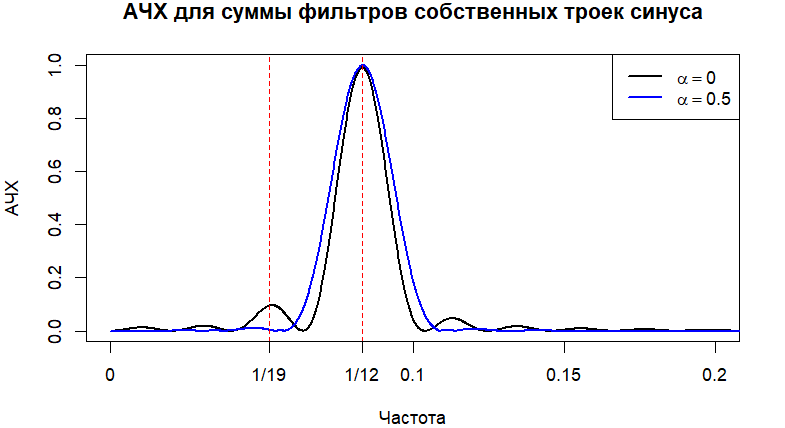
\includegraphics[width=1\textwidth]{img/various_alphas_sin_cos.png}
	\caption{Ряд $\TS = \TS_{\sin} + \TS_{\cos}$. АЧХ фильтров для первых двух компонент (синуса), при разных $\alpha$.}
	\label{fig:various_alphas_sin_cos}
\end{figure}

По рисунку \ref{fig:various_alphas_sin_cos} заметно, что фильтр для синуса в базовом $\SSA$ также частично захватит периодику с частотой $\frac{1}{19}$, в то время, как $\GSSA$ не будет испытывать таких проблем.

\subsection{Фильтры в различных точках}
В зависимости от точек ряда, линейные фильтры будут отличаться друг от друга. Рассмотрим тот же пример $\TS = \TS_{\sin} + \TS_{\cos} + \TS_{\mathrm{noise}} =
	\sin\left(\frac{2\pi}{12}x\right) +
	\frac{1}{2}\cos\left(\frac{2\pi}{19}x\right)+
	\varepsilon_n$,
где $\varepsilon_n \sim \mathrm N(0, 0.1^2)$.
\begin{figure}[H]
	\centering
	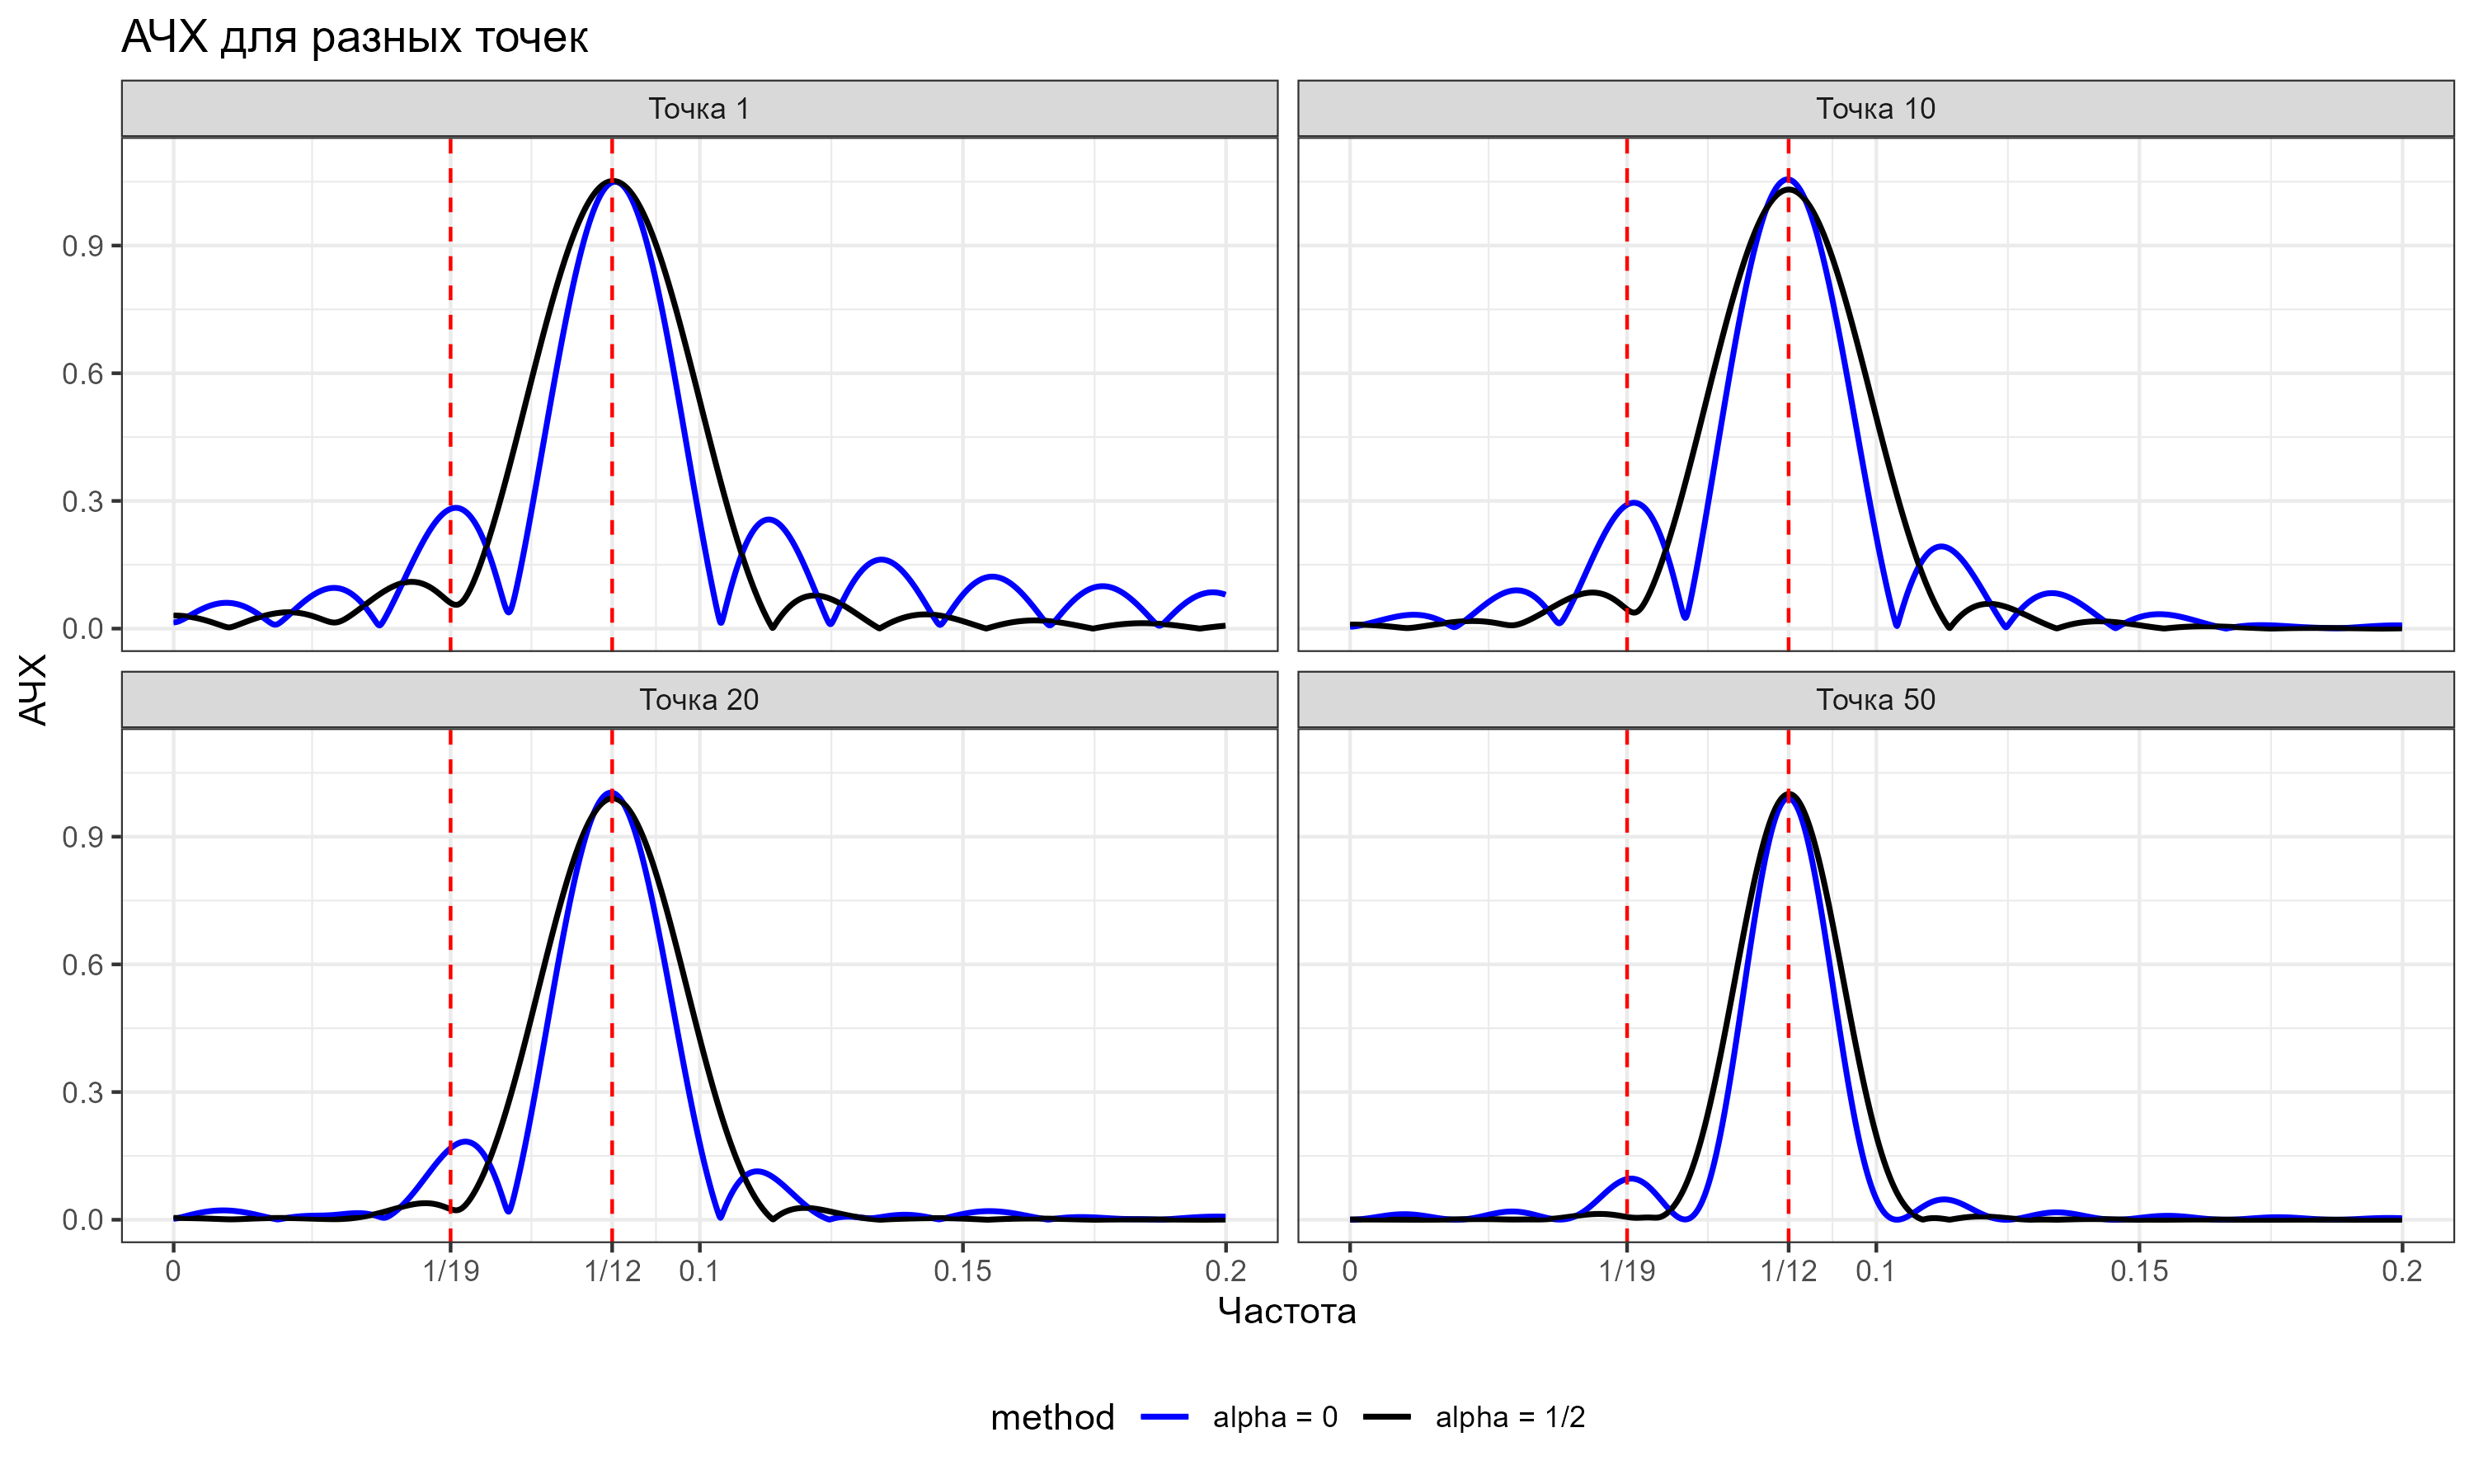
\includegraphics[width=1\textwidth]{img/afc_4_points.png}
	\caption{Ряд $\TS = \TS_{\sin} + \TS_{\cos}+ \TS_{\mathrm{noise}}$. АЧХ фильтров в разных точках, для первых двух компонент при разных $\alpha$.}
	\label{fig:filter_point_depends}
\end{figure}

По рисунку \ref{fig:filter_point_depends} видно, что когда точка s приближается по времени к средним точкам временного ряда ($L \leq s \leq K$), полоса пропускания фильтра становится уже, а также фильтр начинает все меньше и меньше захватывать соседние частоты.

Для этого примера также можно посмотреть на график средней MSE ошибки в зависимости от точки ряда. Эксперимент проводился 1000 раз.
\begin{figure}[H]
	\centering
	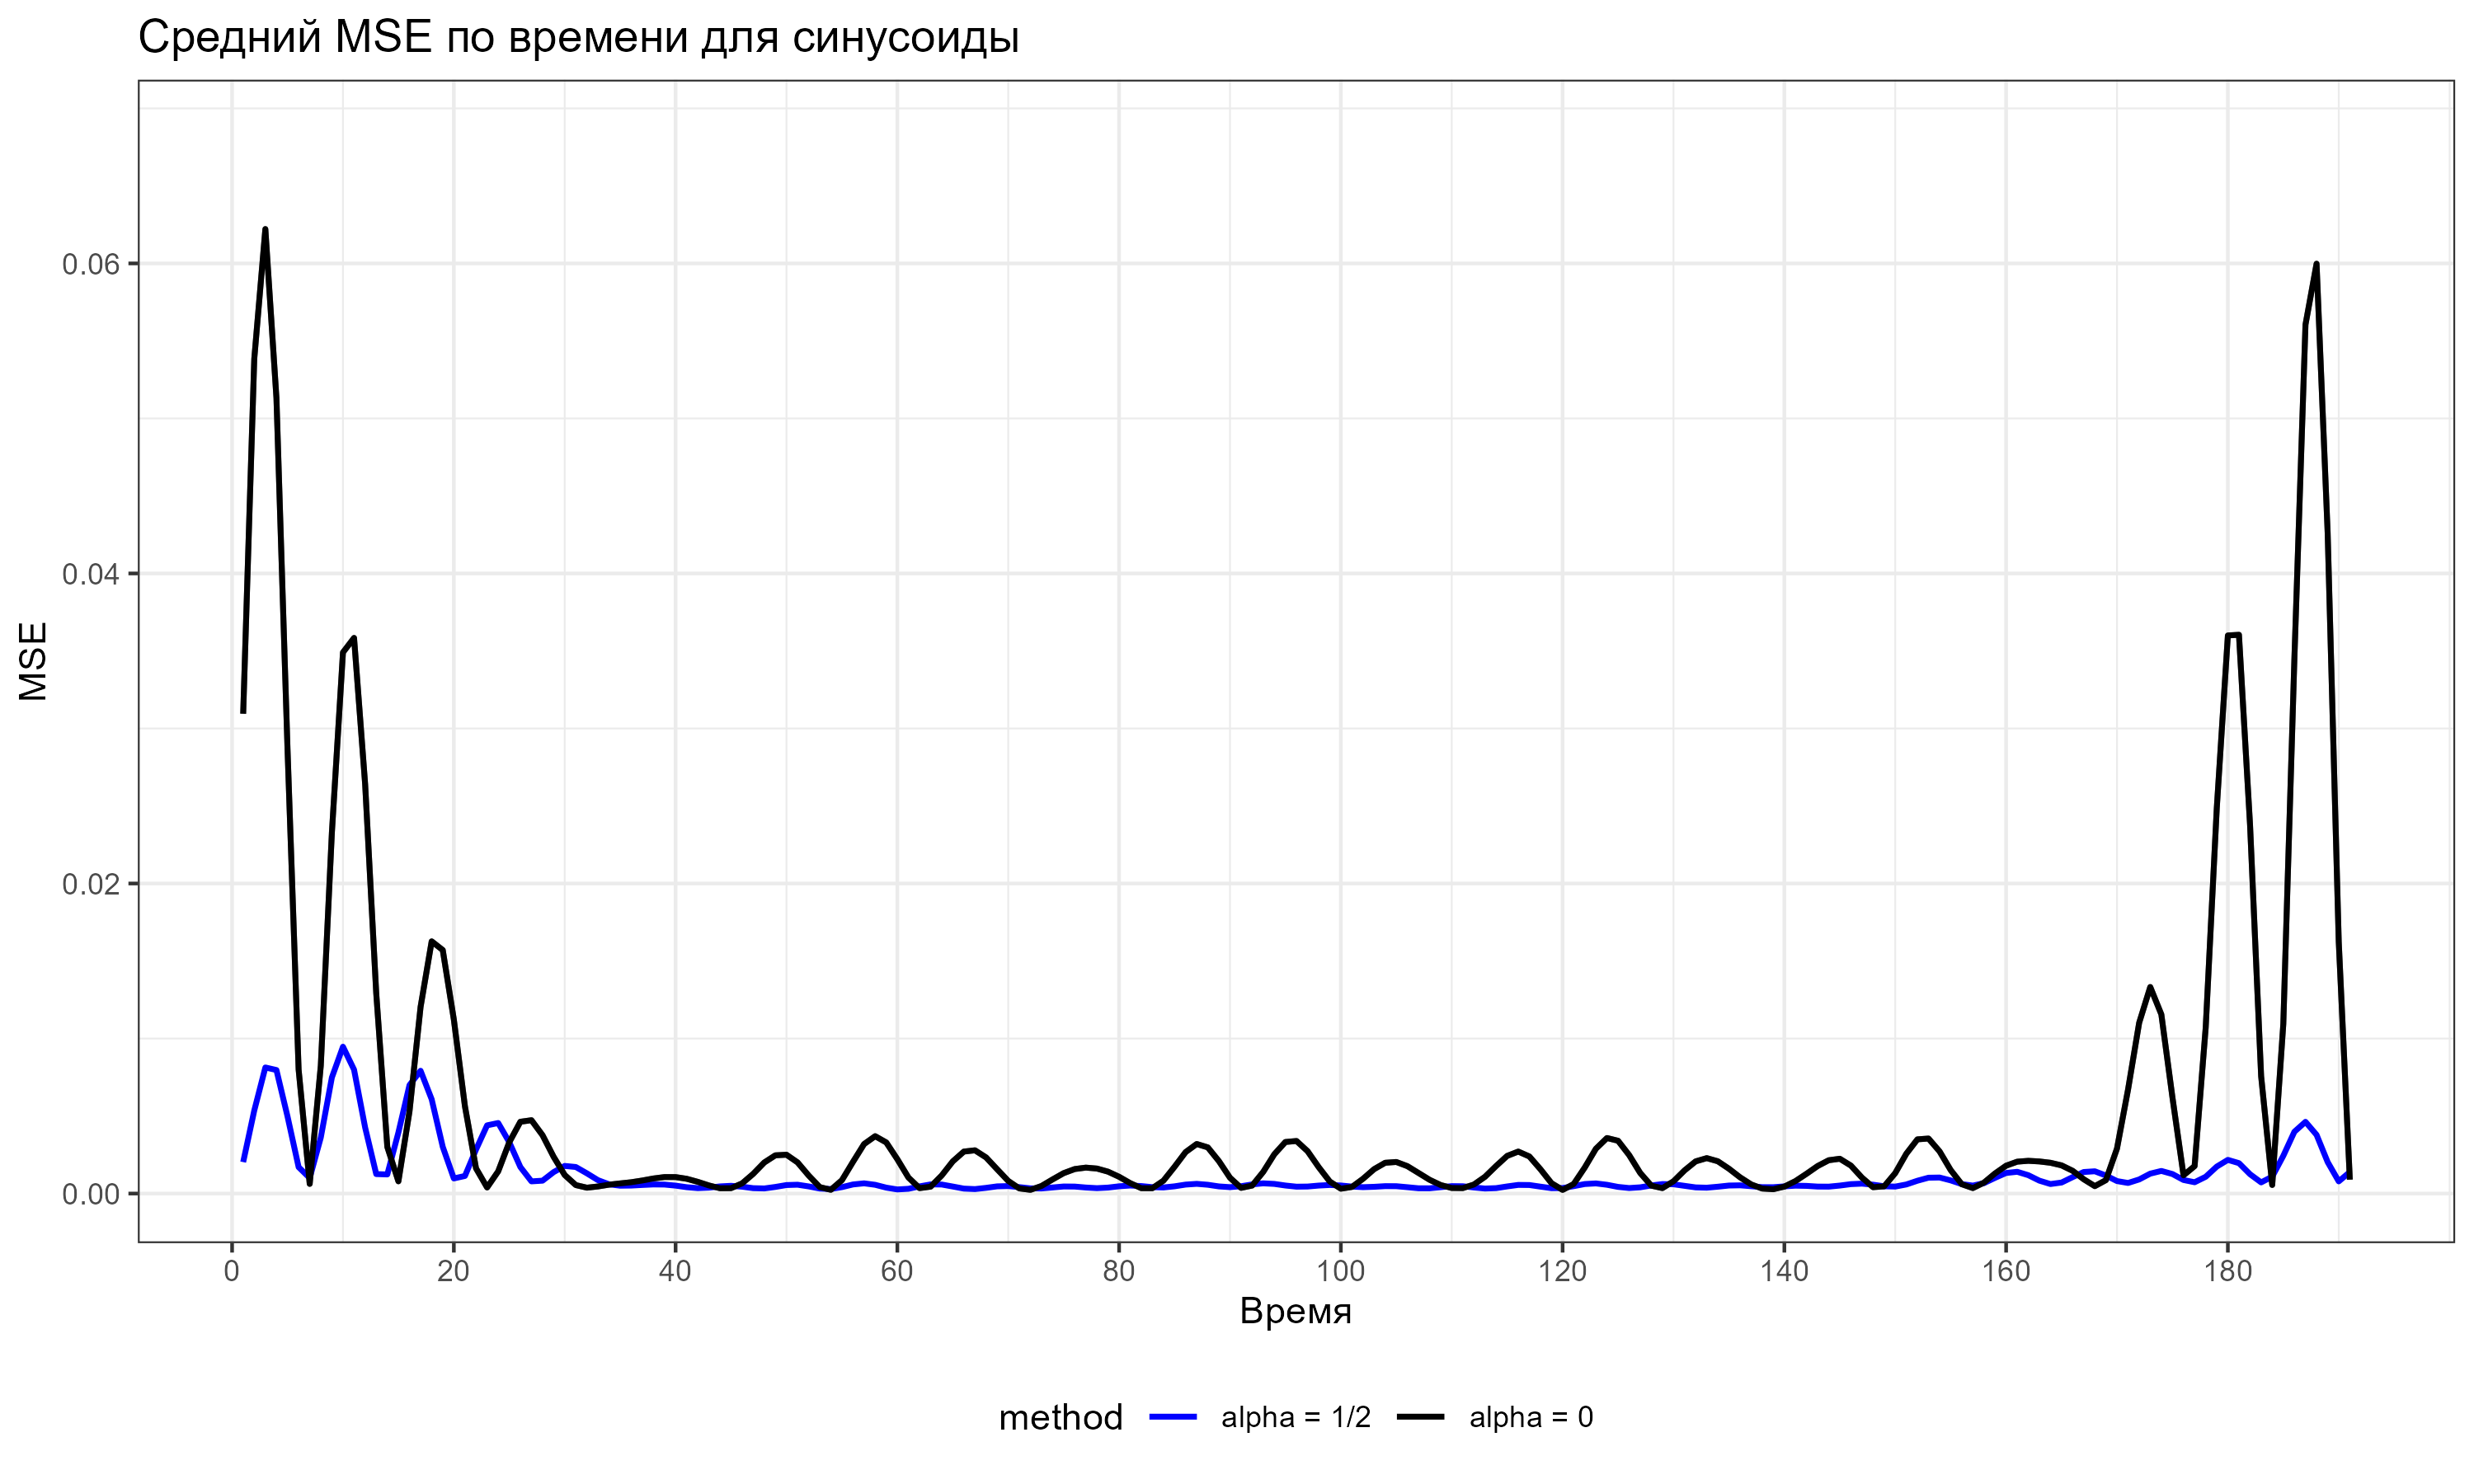
\includegraphics[width=1\textwidth]{img/mse_y1_time.png}
	\caption{Ряд $\TS = \TS_{\sin} + \TS_{\cos}+ \TS_{\mathrm{noise}}$. MSE ошибки для первых двух компонент в зависимости от точки ряда.}
	\label{fig:mse_filter_point_depends}
\end{figure}

Таким образом, можно сделать вывод, что разделимость также зависит от точки ряда. В средних точках достигаются наилучшие значения ошибки. Однако это не означает, что нужно брать маленькое $L$, поскольку чем больше длина окна, тем лучше происходит разделение компонент между собой в целом \cite{golyandina2001analysis}.











\subsection{Влияние шума}

Теперь посмотрим на общую ошибку для примера $\TS = \TS_{\sin} + \TS_{\cos}$.

\begin{table}[H]
	\caption{MSE разложений ряда $\TS = \TS_{\sin} + \TS_{\cos}$ для $\SSA$ и $\GSSA$ с $\alpha = \frac{1}{2}$.}
	\centering
	\begin{tabular}{c|ccc}
		\hline
		Метод/Ошибка                  & $\TS_{\sin}$      & $\TS_{\cos}$      & $\TS$             \\
		\hline
		$\SSA$                  & 5.15e-03          & 5.15e-03          & \textbf{6.01e-30} \\
		$\GSSA$, $\alpha = 0.5$ & \textbf{3.68e-04} & \textbf{3.68e-04} & \textbf{9.53e-30} \\
		\hline
	\end{tabular}

	\label{tab:mse_ssa_gssa}
\end{table}

В таблице \ref{tab:mse_ssa_gssa} жирным выделены наилучшие результаты ошибки. По ней видно, что $\GSSA$ справился с разделением на порядок лучше $\SSA$.

Однако, у $\GSSA$ есть другая проблема. Если добавить к ряду шум, то оба алгоритма будут относить к синусу часть шума, пропускаемую фильтром, а для $\GSSA$ диапазон пропускаемых частот шире, поэтому для $\GSSA$ больше шума попадет в компоненты, отвечающие за периодики.

Добавим к $\TS$ шумовую компоненту: \[\TS = \TS_{\sin} + \TS_{\cos} + \TS_{\mathrm{noise}} =
	\left\{
	\sin\left(\frac{2\pi}{12}n\right) +
	\frac{1}{2}\cos\left(\frac{2\pi}{19}n\right)+
	\varepsilon_n, \,
	n = 1, \dots, N
	\right\}, \]
где $\varepsilon_n \sim \mathrm N(0, 0.1^2)$, $N = 96 \cdot 2 - 1$, $L = 48$.
Проводилось $100$ тестов, в таблице \ref{tab:errs_ssa_gssa} указаны средние значения ошибки для одних и тех же реализаций шума.


\begin{table}[H]
	\caption{MSE разложений ряда $\TS = \TS_{\sin} + \TS_{\cos} + \TS_{\mathrm{noise}}$ для $\SSA$ и $\GSSA$ с $\alpha = \frac{1}{2}$.}
	\label{tab:errs_ssa_gssa}
	\centering
	\begin{tabular}{c|ccc}
		\hline
		Метод                                 & $\TS_{\sin}$      & $\TS_{\cos}$      & $\TS$             \\
		\hline
		$\SSA$                         & 5.68e-03          & 5.44e-03          & \textbf{7.48e-04} \\
		$\GSSA$, $\alpha = \frac{1}{2}$ & \textbf{1.21e-03} & \textbf{1.25e-03} & 1.04e-03          \\
		\hline
	\end{tabular}

\end{table}

В таблице \ref{tab:errs_ssa_gssa} жирным отмечены наилучшие результаты ошибки. По ней видно, что $\GSSA$ все же справился лучше $\SSA$, однако порядок ошибки теперь одинаковый для рассмотрения косинуса или синуса. Но при этом, отделение сигнала от шума получилось лучше у $\SSA$.
Также был проведен парный t-критерий для зависимых выборок с целью проверки гипотезы о равенстве средних значений ошибки для каждой компоненты. В качестве нулевой гипотезы ($H_0$) предполагалось, что средние значения сравниваемых выборок из величин ошибок равны. Уровень значимости был установлен на уровне $\alpha_{\mathrm{hypothesis}} = 0.05$.
Результаты анализа показали, что во всех случаях $p$-значение оказалось меньше 0.05, что позволяет отвергнуть нулевую гипотезу.

\subsection{Вложенный вариант}
Сингулярное разложение матрицы обладает наилучшими аппроксимационными свойствами в смысле минимизации нормы Фробениуса (или спектральной нормы) для заданного ранга. Из этого следует, что разложение матрицы $\mathbf{S} = \mathbf{X}\mathbf{X}^{\mathrm{T}}$ методом SVD будет наилучшим образом отделять сигнал от шума.

По результатам сравнений методов из таблиц \ref{tab:mse_ssa_gssa} и \ref{tab:errs_ssa_gssa}, а также предыдущих рассуждений, получается, что есть смысл использовать базовый $\SSA$ для выделения сигнала, а уже сам сигнал разделять на различные компоненты с помощью $\GSSA$.

Рассмотрим \[\TS = \TS_{\sin} + \TS_{\cos} + \TS_{\mathrm{noise}} =
	\left\{
	\sin\left(\frac{2\pi}{12}n\right) +
	\frac{1}{2}\cos\left(\frac{2\pi}{19}n\right)+
	\varepsilon_n, \,
	n = 1, \dots, N
	\right\}, \]
где $\varepsilon_n \sim \mathrm N(0, 0.1^2)$, только теперь сначала применим $\SSA$, а затем $\GSSA$. Получится вложенный вариант.
$N = 96 \cdot 2 - 1$, $L = 48$ для обоих методов.

\begin{table}[H]
	\centering
	\caption{$\TS_{\sin} + \TS_{\cos}+
			\varepsilon_n$, $\varepsilon_n \sim \mathrm N(0, 0.1^2)$, MSE оценок. }
	\label{tab:errs_ssa_gssa_unite}
	\begin{tabular}{l|ccc}
		\hline
		Метод/Ошибка                     & $\TS_{\sin}$      & $\TS_{\cos}$      & $\TS$             \\
		\hline
		$\SSA$                           & 5.68e-03          & 5.44e-03          & \textbf{7.48e-04} \\
		$\GSSA$, $\alpha = 0.5$          & \textbf{1.21e-03} & \textbf{1.25e-03} & 1.04e-03          \\
		\hline
		$\SSA$ + $\GSSA$, $\alpha = 0.5$ & \textbf{1.06e-03} & \textbf{1.12e-03} & \textbf{7.15e-04} \\
		\hline
	\end{tabular}
\end{table}

Анализ данных, представленных в таблице \ref{tab:errs_ssa_gssa_unite}, позволяет сделать вывод, что комбинирование алгоритмов привело к улучшению как в выделении полезного сигнала, так и в разделении компонент между собой. Полученные результаты демонстрируют более высокую точность по сравнению с данными, приведёнными в таблице \ref{tab:errs_ssa_gssa}.


Таким образом, по приведенным примерам можно сделать вывод, что $\GSSA$ позволяет улучшить разделимость периодических компонент ряда. Однако, вместе с тем, разложение будет захватывать больше шума в сравнении с базовым $\SSA$.




\newpage





\section{Различия SSA, CiSSA и Фурье}

\label{sec:comparison_cissa}
В данной секции проводится сравнение методов разложения временного ряда: базовый $\SSA$,  $\SSA$ с использованием EOSSA для улучшения разделимости, разложения Фурье и Фурье с расширением ряда, базового $\CISSA$ и $\CISSA$ с расширением ряда. Все вычисления, а также код метода $\CISSA$ можно найти в репозитории \cite{spbu_cissa_coursework_github}


\subsection{Автоматическая группировка}

\label{subsubsec:autogroup}

Авторы статьи \cite{bogalo2020} выделяют главным преимуществом то, что $\CISSA$ автоматически разделяет компоненты ряда по частотам. Однако есть метод, позволяющий сделать автоматическое объединение частот по периодограмме в методе $\SSA$
\cite{golyandina2023automatedidentificationsingularspectrum}
. При этом, прежде чем применять его, стоит выполнить процедуру улучшения разделимости. В данной работе будут использоваться методы EOSSA и FOSSA \cite{golyandina2023intelligent}. Отсюда следует, что все рассматриваемые в данной секции алгоритмы могут по заранее заданным диапазонам частотам выдать временные ряды, отвечающие за эти диапазоны.



\subsection{Собственные пространства}
Каждый алгоритм после группировки порождает собственные подпространства. В случае базового $\SSA$ базис подпространств является адаптивным, то есть зависящим от $\TS, L, N$.

В случае $\CISSA$ базис зависит только от $L, N$. Если зафиксировать данные параметры, и менять $\TS$, базис никак не поменяется.

На базис разложения Фурье влияет только $N$.


\subsection{Выбор длины окна для CiSSA}
\label{subsec:cissa_L_choice}

Фиксируем временной ряд $\TS = \left(x_1, \cdots, x_N\right)$ длины $N$, а также набор интересующих частот $\Omega = \left\{\omega_k: \omega_k \in [0, 0.5] \right\}$ и соответствующие диапазоны $\Omega_j$:
		      $\bigsqcup \limits_{j=1}^m \Omega_j =
			      \bigsqcup \limits_{j=1}^m
			      \left[ \omega_j^{(l)}, \omega_j^{(r)} \right] =
			      [0, 0.5]$, $\omega_k \in \Omega_k$.
% Будем рассматривать только случаи, когда $L \omega_k \in \mathbb{N}$ для любого $\omega_k \in \Omega$, а также нет шума.

Возникает вопрос: какое $L$ лучше выбрать?

\subsubsection*{Без шума}

Если ряд состоит только из синусов и косинусов, то по условиям точной разделимости разницы нет, ошибка всегда будет нулевая. Однако, если это не так, то из всех возможных $L$ нужно выбирать наименьшее подходящее, поскольку чем оно меньше, тем более локальные свойства $\CISSA$ будет извлекать из ряда.

В подтверждение этому рассмотрим пример 
\[\TS = \TS_{e\cdot\sin} + \TS_{e\cdot\cos} =  \left\{ e^{A_1 n } \sin(2\pi \omega_1 n ) + e^{A_2 n} \cos(2\pi \omega_2 n ), \, n = 1, \dots, N \right\} \]
 с $A_1 = \frac{1}{200}$, $A_2 = \frac{1}{100}$, $\omega_1 = \frac{1}{12}$, $\omega_2 = \frac{1}{3}$, $N = 96 \cdot 2$. Будем следить за ошибкой в зависимости от длины окна. В качестве $L$ рассмотрим значения, кратные частотам компонентам сигнала. Конкретнее,  $L = 12, 24, 36, 48, 60, 72, 84, 96, 192$.

\begin{figure}[H]
	\centering
	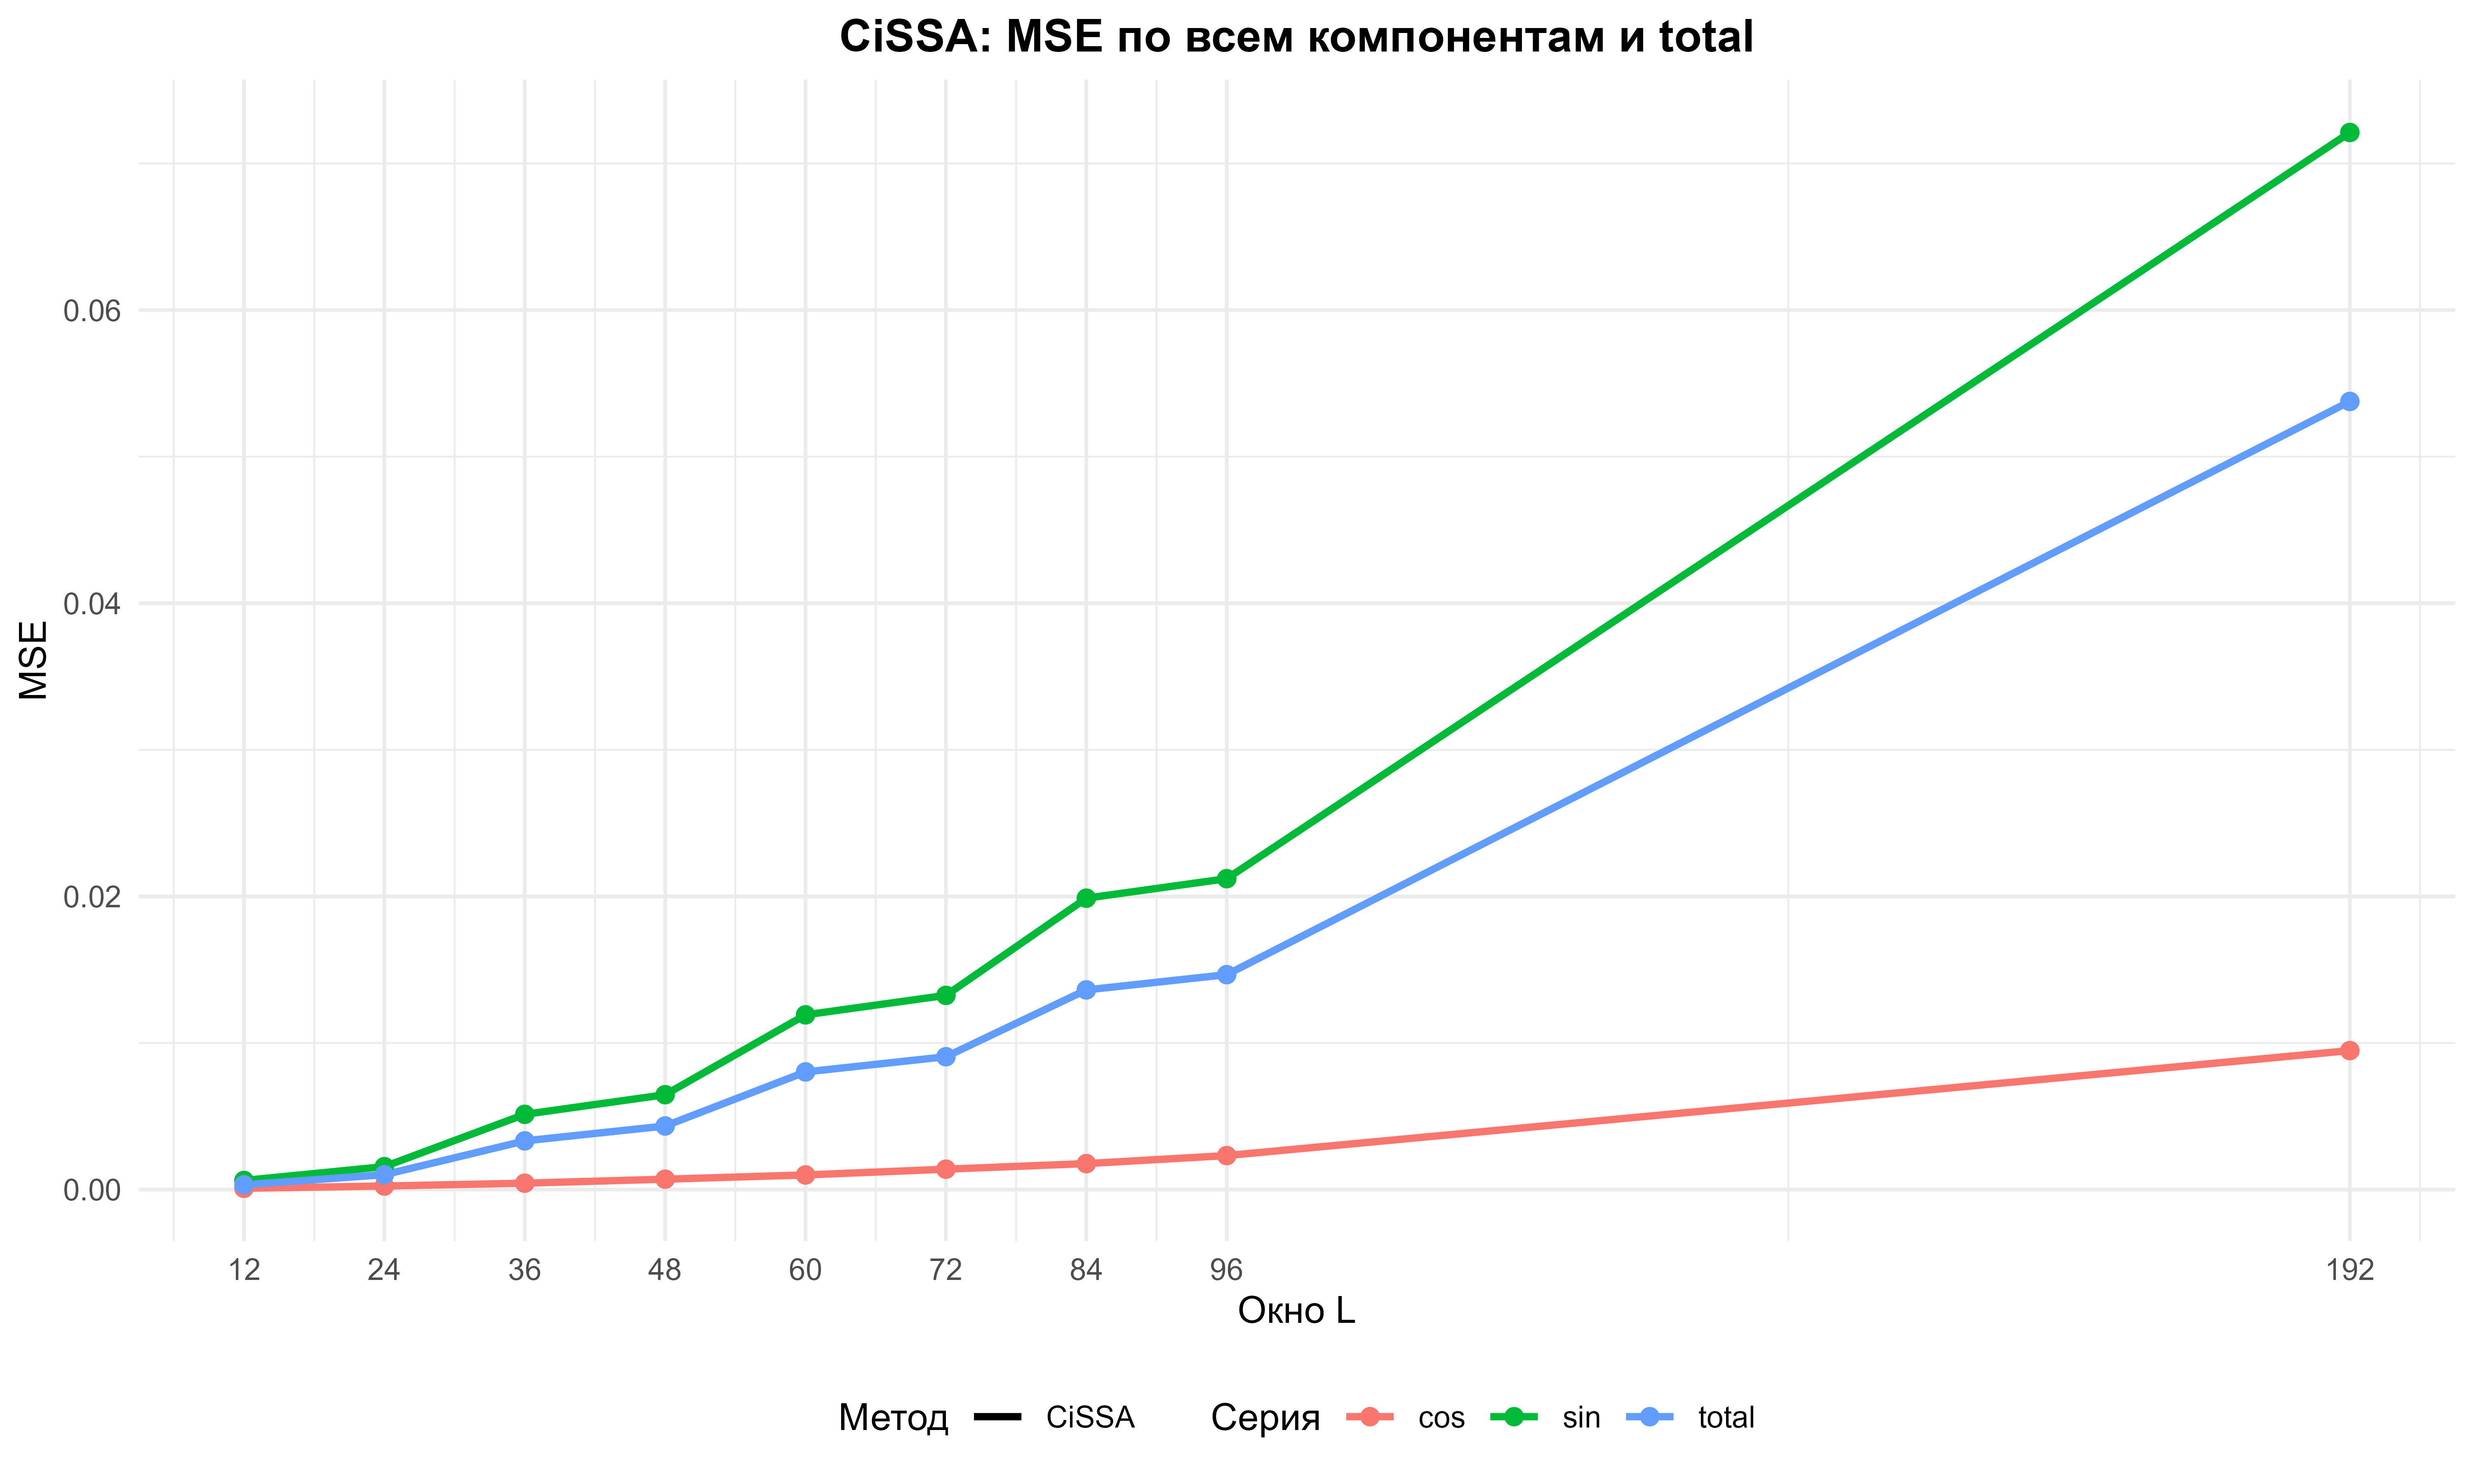
\includegraphics[width=1\textwidth]{img/cissa_errors_plot.png}
	\caption{MSE разделения $\CISSA$ ряда $\TS = \TS_{e\cdot\sin} + \TS_{e\cdot\cos}$ в зависимости от длины окна $L$.}
	\label{fig:cissa_error_depends_on_L}
\end{figure}

Рисунок \ref{fig:cissa_error_depends_on_L} наглядно показывает, что при фиксированном $N$ и с ростом $L$ ошибка увеличивается. При этом, максимума ошибка достигает при $L = 192$, что соответствует обычному применению преобразования Фурье. Кроме того, здесь не важно, по каким диапазонам частот будет произведена группировка, поскольку нет шума. Рассмотрим теперь его влияние.


\subsubsection*{С шумом}

Теперь ошибка для суммы двух гармоник не такие однозначные. Рассмотрим пример с гауссовским шумом.

\[
\TS = \TS_{\sin} + \TS_{\cos} +\TS_{\mathrm{noise}} = \left\{  
A_1 \sin(2\pi \omega_1 n ) + A_2  \cos(2\pi \omega_2 n ) + \varepsilon_n, \, n = 1, \dots, N
\right\},
\] где $\varepsilon_n \sim \mathrm N(0, 1)$, $A_1 = 1$, $A_2 = 0.5$, $\omega_1 = \frac{1}{12}$, $\omega_2 = \frac{1}{3}$, $N = 96 \cdot 2$. Восстановление проводилось по диапазонам $[\omega_i \pm 2 \cdot \frac{1}{193}]$. Было проведено 100 экспериментов и результаты усреднялись для соответствующих компонент и $L$. В качестве $L$ рассмотрим значения, кратные частотам компонентам сигнала. Конкретнее,  $L = 12, 24, 36, 48, 60, 72, 84, 96, 192$.


\begin{figure}[H]
	\centering
	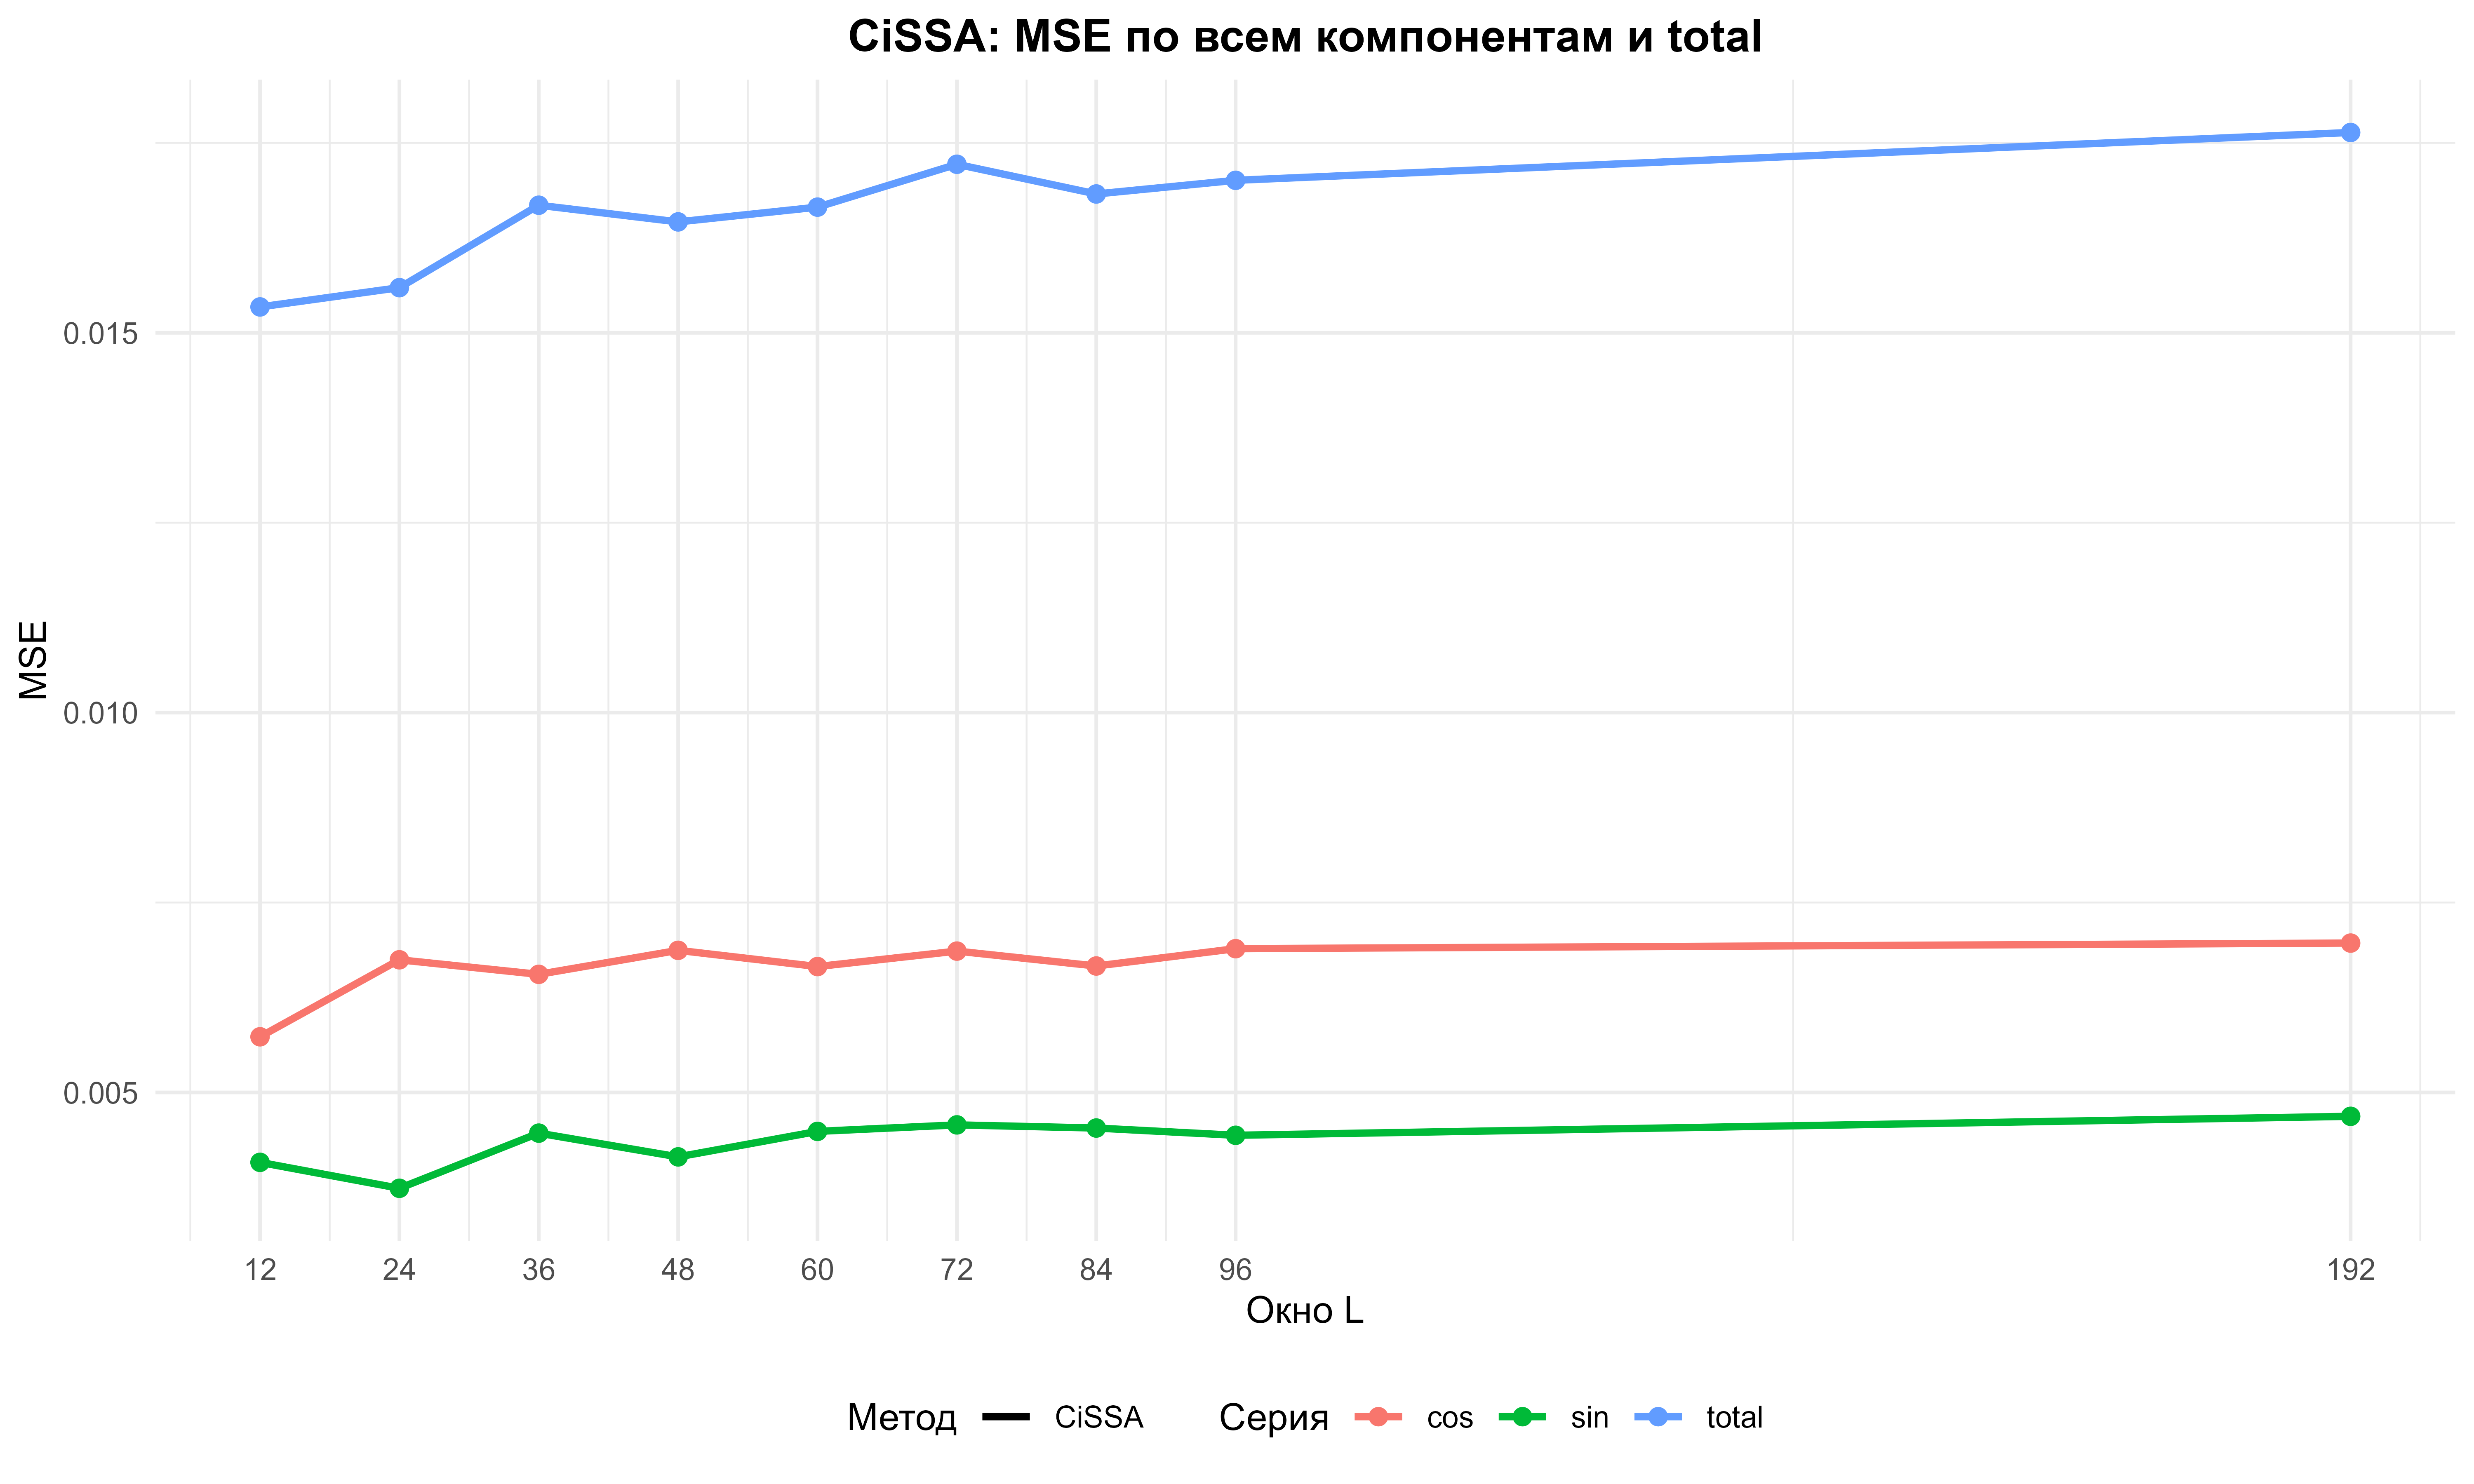
\includegraphics[width=1\textwidth]{img/cissa_errors_plot_cos_noised.png}
	\caption{MSE разделения $\CISSA$ ряда $\TS = \TS_{\sin} + \TS_{\cos} +\TS_{\mathrm{noise}}$ в зависимости от длины окна $L$.}
	\label{fig:cissa_error_cos_noised_depends_on_L}
\end{figure}


Как видно по рисунку \ref{fig:cissa_error_cos_noised_depends_on_L}, ситуация поменялась. Ошибка начинает снижаться с ростом длины окна. Это основано на смещении и дисперсии оценки (\ref{subsec:cissa_fixed_basis_problems}). Дисперсия оценки снижается, а смещение в данном случае никак не меняется с ростом окна.

Теперь рассмотрим пример с экспоненциальной модуляцией: 
\[ 
\TS = \TS_{e\cdot\sin} + \TS_{e\cdot\cos} = 
\left\{
	e^{A_1 n } \sin(2\pi \omega_1 n ) + e^{A_2 n} \cos(2\pi \omega_2 n ) + \varepsilon_n, \, n = 1, \dots, N 
\right\}.
\] 
 $\varepsilon_n \sim \mathrm N(0, 1)$ с $A_1 = \frac{1}{200}$, $A_2 = \frac{1}{100}$, $\omega_1 = \frac{1}{12}$, $\omega_2 = \frac{1}{3}$, $N = 96 \cdot 2$. Восстановление проводилось по диапазонам $[\omega_i \pm 4 \cdot \frac{1}{193}]$. Было проведено 100 экспериментов и результаты усреднялись для соответствующих компонент и $L$. В качестве $L$ рассмотрим значения, кратные частотам компонентам сигнала. Конкретнее,  $L = 12, 24, 36, 48, 60, 72, 84, 96, 192$.

\begin{figure}[H]
	\centering
	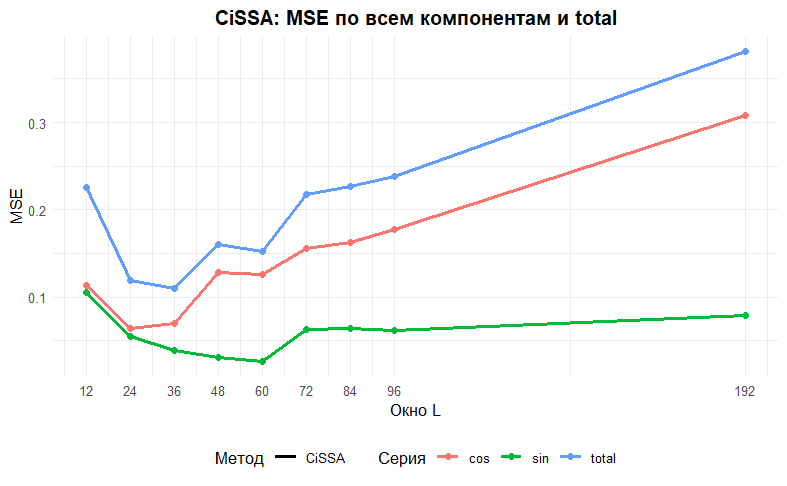
\includegraphics[width=1\textwidth]{img/cissa_errors_plot_expcos_noised.png}
	\caption{MSE разделения $\CISSA$ ряда $\TS = \TS_{e\cdot\sin} + \TS_{e\cdot\cos} + \varepsilon_n$ в зависимости от длины окна $L$ с $[\omega_i \pm 4 \cdot \frac{1}{193}]$.}
	\label{fig:cissa_error_expcos_noised_depends_on_L}
\end{figure}


По рисунку \ref{fig:cissa_error_expcos_noised_depends_on_L} можно увидеть, как борются два эффекта — увеличение смещения и уменьшение дисперсии оценки при росте $L$. 

Кроме того, здесь проявляется проблема фиксированного базиса из раздела \ref{subsec:cissa_fixed_basis_problems}. Если взять тот же пример \[ 
\TS = \TS_{e\cdot\sin} + \TS_{e\cdot\cos} = 
\left\{
	e^{A_1 n } \sin(2\pi \omega_1 n ) + e^{A_2 n} \cos(2\pi \omega_2 n ) + \varepsilon_n, \, n = 1, \dots, N 
\right\},
\] 
где 
 $\varepsilon_n \sim \mathrm N(0, 1)$ с $A_1 = \frac{1}{200}$, $A_2 = \frac{1}{100}$, $\omega_1 = \frac{1}{12}$, $\omega_2 = \frac{1}{3}$, $N = 96 \cdot 2$, но восстановление проводить по диапазонам $[\omega_i \pm 2 \cdot \frac{1}{193}]$, то картина ошибки будет выглядеть иначе.

 \begin{figure}[H]
	\centering
	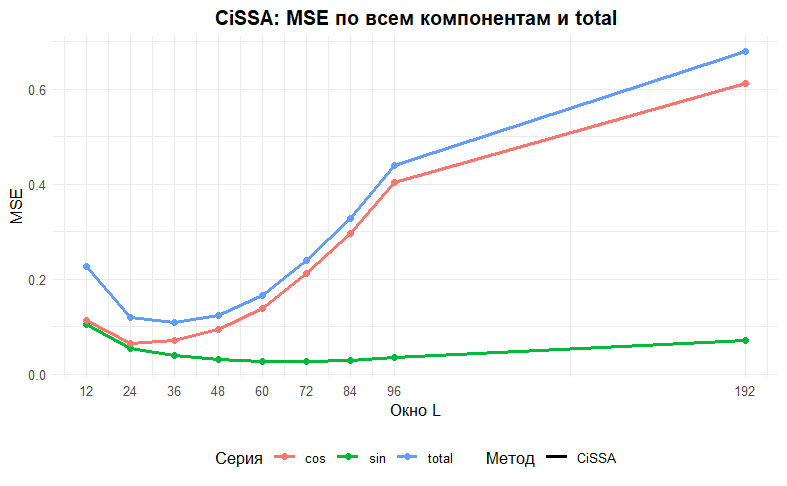
\includegraphics[width=1\textwidth]{img/cissa_errors_plot_expcos_noised_2.png}
	\caption{MSE разделения $\CISSA$ ряда $\TS = \TS_{e\cdot\sin} + \TS_{e\cdot\cos} + \varepsilon_n$ в зависимости от длины окна $L$ с $[\omega_i \pm 2 \cdot \frac{1}{193}]$.}
	\label{fig:cissa_error_expcos_noised_depends_on_L_2}
\end{figure}


Из рисунков \ref{fig:cissa_error_expcos_noised_depends_on_L} и \ref{fig:cissa_error_expcos_noised_depends_on_L_2} можно сделать вывод, что в силу неадаптивности базиса исследователю нужно очень аккуратно выбирать диапазоны частот, по которым следует объединять компоненты.


\subsection{Без шума}
\label{subsec:cissa_examples_without_noise}

В данном разделе будем рассматривать результаты сравнений для временного ряда, состоящего только из сигнала.



\subsubsection{Гармонические функции}
\label{subsubsec:exact}

В свойствах методов были приведены классы функций и условия, при которых методы могут безошибочно разделить два ряда друг от друга. Сравним эти условия.


Фиксируем временной ряд, состоящий из двух периодических компонент с постоянной модуляцией  $\TS = \TS_{1} + \TS_{2} =$ $A_1 \cos(2\pi \omega_1 n + \varphi_1) + A_2 \cos(2\pi \omega_2 n + \varphi_2)$.

\begin{table}[H]
    \centering
    \caption{Условия точной разделимости для $\SSA$, $\EOSSA$, $\FOURIER$, $\CISSA$.}
    \label{tab:separability_conditions}
    \begin{tabular}{l|c}
        \hline
        \textbf{Метод}     & \textbf{Условия точной разделимости} \\
        \hline
        $\SSA$     & $L\omega_1, L\omega_2, K\omega_1, K\omega_2 \in \mathbb{N}$, $\omega_1 \ne \omega_2$, $A_1 \ne A_2$ \\
        $\EOSSA$ & $\omega_1 \ne \omega_2$ \\
        $\FOURIER$     & $N\omega_1, N\omega_2 \in \mathbb{N}$, $\omega_1 \ne \omega_2$ \\
        $\CISSA$     & $L\omega_1, L\omega_2 \in \mathbb{N}$, $\omega_1 \ne \omega_2$ \\
        \hline
    \end{tabular}
\end{table}

Из таблицы \ref{tab:separability_conditions} видно, что для самые жесткие условия для $\SSA$, а наилучшие у $\EOSSA$.  Для $\FOURIER$ и $\CISSA$ условия схожи, однако тут стоит отметить, что длину ряда $N$ далеко не всегда можно подобрать, в отличие от $L$. В этом смысле лучше себя показывает $\CISSA$ в сравнении с $\FOURIER$.

Теперь посмотрим численно, на следующие ситуации: параметры рассматриваемых методов подобраны верно, параметры подобраны плохо.


% Разложение Фурье может отличить друг от друга периодические компоненты, попадающие в решетку его частот. Другими словами, разложением Фурье может быть точно разделен ряд $\TS = \TS_{w_1} + \TS_{w_2}$, где $\TS_{w_1} = A_1 \cos(2\pi w_1 n + \varphi_1)$, $\TS_{w_2} = A_2 \cos(2\pi w_2 n + \varphi_2)$ и $Nw_1, Nw_2 \in \mathbb{N}$, $w_1 \not = w_2$.

% Похожие условия точной разделимости у метода $\CISSA$. С помощью данного алгоритма может быть точно разделен ряд $\TS = \TS_{w_1} + \TS_{w_2}$, где $\TS_{w_1} = A_1 \cos(2\pi w_1 n + \varphi_1)$, $\TS_{w_2} = A_2 \cos(2\pi w_2 n + \varphi_2)$, только $Lw_1, Lw_2 \in \mathbb{N}$, $w_1 \not = w_2$.

% У алгоритма $\SSA$ для разделения $\TS = \TS_{w_1} + \TS_{w_2}$ накладываются более жесткие ограничения:  $Lw_1, Lw_2, Kw_1, Kw_2 \in \mathbb{N}$, $w_1 \not = w_2$, $A_1 \not = A_2$. Однако также могут быть точно разделены ряды $\TS = \TS_{\exp_1} + \TS_{\exp_2} = A_1 \exp(\alpha_1 n)\cos(2\pi w_1 n + \varphi_1) + A_2 \exp(\alpha_2 n)\cos(2\pi w_2 n + \varphi_2)$, где $Lw_1, Lw_2, Kw_1, Kw_2 \in \mathbb{N}$, $w_1 \not = w_2$, $A_1 \not = A_2$, $\alpha_1 \not = \alpha_2$.

\textbf{\large{Пример.}} Будем разделять временной ряд 
\[ \TS = \TS_{\sin} + \TS_{\cos} = 
\left\{ 
	\sin{\frac{2\pi}{12}n} + \frac{1}{2}\cos{\frac{2\pi}{3}n}, \, n = 1, \dots, N \right\}.\]
% \textbf{\large{Пример.}} Будем разделять временной ряд 
% \(\TS = \TS_{\sin} + \TS_{\cos} = \{\sin(2\pi n/12) + \tfrac12\cos(2\pi n/3)\}\).

\begin{table}[H]
\centering
\caption{MSE разложений \(\TS = \TS_{\sin} + \TS_{\cos}\).}
\label{tab:exact_not_noised_results}
\begin{tabular}{l|c|ccc}
  \hline
  \textbf{Метод} & \textbf{Условия} & \(\MSE(\TS_{\sin})\) & \(\MSE(\TS_{\cos})\) & \(\MSE(\TS)\) \\ 
  \hline
  $\SSA$    & (1) & 6.8e-30 & 1.5e-29 & 1.8e-29 \\ 
  $\SSA$    & (2) & 2.2e-06 & 2.2e-06 & 2.0e-29 \\ 
  \hline
  $\EOSSA$  & (3) & 7.5e-30 & 1.5e-29 & 2.0e-29 \\ 
  $\EOSSA$  & (4) & 8.8e-30 & 1.5e-29 & 1.9e-29 \\ 
  \hline
  $\FOURIER$    & (5) & 3.4e-28 & 1.2e-28 & 4.3e-28 \\ 
  $\FOURIER$ & (6) & 1.2e-03 & 3.1e-03 & 4.1e-03 \\ 
  \hline
  $\CISSA$  & (7) & 5.5e-30 & 1.4e-29 & 8.6e-30 \\ 
  $\CISSA$ & (8) & 5.5e-30 & 1.6e-29 & 1.4e-29 \\ 
  $\CISSA$ & (9) & 2.2e-03 & 5.7e-03 & 6.2e-03 \\ 
  \hline
\end{tabular}
\end{table}

\begin{table}[H]
  \caption{Параметры для таблицы \ref{tab:exact_not_noised_results}.}
  \centering
  \label{tab:exact_not_noised_parameters}
  \begin{tabularx}{\textwidth}{|c|X|}
    \hline
    \textbf{Условия} & \textbf{Параметры} \\
    \hline
    (1) & \( L = 96,\; N = 191 \). \\ & Группы: $\TS_{\sin} - [1,2]; \TS_{\cos} - [3,4]$. \\
    \hline
    (2) & \( L = 96,\; N = 192 \). \\ & Группы: $\TS_{\sin} - [1,2]; \TS_{\cos} - [3,4]$. \\
    \hline
    (3) & \( L = 96,\; N = 191,\; r = 4\). \\
            & Частоты: $\TS_{\sin} - [\omega_1 \pm \varepsilon]; \TS_{\cos} - [\omega_2 \pm \varepsilon]$, $\varepsilon = 6/192$. \\
    \hline
    (4) & \( L = 96,\; N = 192,\; r = 4 \). \\
            & Частоты: $\TS_{\sin} - [\omega_1 \pm \varepsilon]; \TS_{\cos} - [\omega_2 \pm \varepsilon]$, $\varepsilon = 6/192$. \\
    \hline
    (5) & \( N = 192 \). \\
            & Частоты: $\TS_{\sin} - [\omega_1 \pm \varepsilon]; \TS_{\cos} - [\omega_2 \pm \varepsilon]$, $\varepsilon = 6/192$. \\
    \hline
    (6) & \( N = 192 \). \\
            & Частоты: $\TS_{\sin} - [\omega_1 \pm \varepsilon]; \TS_{\cos} - [\omega_2 \pm \varepsilon]$, $\varepsilon = 6/192$. \\
    \hline
    (7) & \(L = 12,\;N = 192 \). \\
            & Частоты: $\TS_{\sin} - [\omega_1 \pm \varepsilon]; \TS_{\cos} - [\omega_2 \pm \varepsilon]$, $\varepsilon = 6/192$. \\
    \hline
    (8) & \( L = 96,\; N = 192 \). \\
            & Частоты: $\TS_{\sin} - [\omega_1 \pm \varepsilon]; \TS_{\cos} - [\omega_2 \pm \varepsilon]$, $\varepsilon = 6/192$. \\
    \hline
    (9) & \( L = 97,\; N = 192 \). \\
            & Частоты: $\TS_{\sin} - [\omega_1 \pm \varepsilon]; \TS_{\cos} - [\omega_2 \pm \varepsilon]$, $\varepsilon = 6/192$. \\
    \hline
  \end{tabularx}
\end{table}


По результатам таблицы \ref{tab:exact_not_noised_results} видно, что все алгоритмы при нарушении условий точной разделимости перестают отделять компоненты друг от друга с точностью машинного нуля. Однако в следствии частотной разделимости, ошибка все равно мала. Меньше всего при нарушении условий точной разделимости ошибка для $\SSA$, на 3 порядка хуже у $\CISSA$ и $\FOURIER$.



\subsubsection{Экспоненциально-модулированные функции}


Как следствие асимптотической разделимости можно рассмотреть следующий пример.

\textbf{\large{Пример.}} Будем разделять временной ряд 
\[ 
\TS = \TS_{e \cdot \sin} + \TS_{e \cdot \cos} = \{e^{n/200}\sin(2\pi n/12) + e^{n/100}\cos(2\pi n/3), n = 1, \dots, N\}.
\]

\begin{table}[H]
\centering
\caption{MSE разложений \(\TS = \TS_{e \cdot \sin} + \TS_{e \cdot \cos}\).}
\label{tab:exp_mod_results}
\begin{tabular}{l|c|ccc}
  \hline
  \textbf{Метод} & \textbf{Условия} & \(\MSE(\TS_{\sin})\) & \(\MSE(\TS_{\cos})\) & \(\MSE(\TS)\) \\ 
  \hline
  $\SSA$    & (1) & 5.3e-05 & 5.3e-05 & 1.2e-27 \\ 
  $\SSA$    & (2) & 1.8e-04 & 1.8e-04 & 1.1e-27 \\ 
  \hline
  $\EOSSA$  & (3) & 8.3e-29 & 1.2e-27 & 1.1e-27 \\ 
  $\EOSSA$  & (4) & 8.4e-29 & 1.2e-27 & 1.1e-27 \\ 
  \hline
  $\FOURIER$    & (5) & 1.5e-02 & 8.6e-02 & 7.9e-02 \\ 
  $\FOURIER$ & (6) & 9.4e-03 & 1.2e-01 & 1.3e-01 \\ 
  \hline
  $\CISSA$  & (7) & 5.7e-05 & 1.2e-03 & 1.0e-03 \\ 
  $\CISSA$ & (8) & 3.1e-03 & 4.2e-02 & 3.5e-02 \\ 
  $\CISSA$ & (9) & 1.2e-02 & 1.5e-01 & 1.1e-01 \\ 
  \hline
\end{tabular}
\end{table}

\begin{table}[H]
  \caption{Параметры для таблицы \ref{tab:exp_mod_results}.}
  \centering
  \label{tab:exp_mod_parameters}
  \begin{tabularx}{\textwidth}{|c|X|}
    \hline
    \textbf{Условия} & \textbf{Параметры} \\
    \hline
    (1) & \(L = 96,\; N = 191\). \\ 
        & Группы: \(\TS_{e \cdot \sin}\) —  \([3,4]\); \(\TS_{e \cdot \cos}\) —  \([1,2]\). \\
    \hline
    (2) & \(L = 96,\; N = 192\). \\ 
        & Группы: \(\TS_{e \cdot \sin}\) —  \([3,4]\); \(\TS_{e \cdot \cos}\) —  \([1,2]\). \\
    \hline
    (3) & \(L = 96,\; N = 191,\; r = 4\). \\ 
       & Частоты: $\TS_{e \cdot \sin} - [\omega_1 \pm \varepsilon]; \TS_{e \cdot \cos} - [\omega_2 \pm \varepsilon]$, $\varepsilon = 10/192$. \\
    \hline
    (4) & \(L = 96,\; N = 192,\; r = 4\). \\ 
        & Частоты: $\TS_{e \cdot \sin} - [\omega_1 \pm \varepsilon]; \TS_{e \cdot \cos} - [\omega_2 \pm \varepsilon]$, $\varepsilon = 10/192$. \\
    \hline
    (5) & \(N = 192\). \\ 
        & Частоты: $\TS_{e \cdot \sin} - [\omega_1 \pm \varepsilon]; \TS_{e \cdot \cos} - [\omega_2 \pm \varepsilon]$, $\varepsilon = 10/192$. \\
    \hline
    (6) & \(N = 191\). \\ 
        & Частоты: $\TS_{e \cdot \sin} - [\omega_1 \pm \varepsilon]; \TS_{e \cdot \cos} - [\omega_2 \pm \varepsilon]$, $\varepsilon = 10/192$. \\
    \hline
    (7) & \(L = 12,\; N = 192\). \\ 
        & Частоты: $\TS_{e \cdot \sin} - [\omega_1 \pm \varepsilon]; \TS_{e \cdot \cos} - [\omega_2 \pm \varepsilon]$, $\varepsilon = 10/192$. \\
    \hline
    (8) & \(L = 97,\; N = 192\). \\ 
       & Частоты: $\TS_{e \cdot \sin} - [\omega_1 \pm \varepsilon]; \TS_{e \cdot \cos} - [\omega_2 \pm \varepsilon]$, $\varepsilon = 10/192$. \\
    \hline
    (9) & \(L = 96,\; N = 192\). \\ 
        & Частоты: $\TS_{e \cdot \sin} - [\omega_1 \pm \varepsilon]; \TS_{e \cdot \cos} - [\omega_2 \pm \varepsilon]$, $\varepsilon = 10/192$. \\
    \hline
  \end{tabularx}
\end{table}

По таблице \ref{tab:exp_mod_results} видно, что $\CISSA$ все же разделяет ряды, но не так хорошо, как это делает $\SSA$ или тем более $\SSA$ с EOSSA. Совсем плохо показал себя $\FOURIER$. Также видим, что с маленьким $L$ $\CISSA$ справляется с разделением лучше, чем с большим.


\subsubsection{Функции с трендом}



\label{subsubsec:trend}

Рассмотрим, влияние непериодических компонент на разложение ряда.

Базовый алгоритм $\SSA$ может выделять трендовую составляющую за счет своего адаптивного базиса. Для алгоритмов $\CISSA$ и разложения Фурье нужно применять процедуры расширения временного ряда, чтобы использовать их для выделения тренда.

\textbf{\large{Пример.}} Рассмотрим ряд из предыдущего примера и добавим к нему тренд. \[
\TS = \TS_{c} + \TS_e + \TS_{\sin} + \TS_{\cos} = 
\left\{
	1 + e^{\frac{n}{100}} + \sin{\frac{2\pi}{12}n} + \frac{1}{2}\cos{\frac{2\pi}{3}n}, \, n = 1, \dots, N
\right\}, \]

$\TS_{\mathrm{trend}} = \TS_{c} + \TS_e$.
%Для каждого алгоритма параметры выбраны таким способом, чтобы получить наилучший результат. \textbf{\large{Пример.}} Будем разделять временной ряд 
% \[
% \TS = \TS_{\text{trend}} + \TS_{\sin} + \TS_{\cos}
% = \{1 + e^{n/100}\} + \{\sin(2\pi n/12)\} + \{\tfrac12\cos(2\pi n/3)\}.
% \]

\begin{table}[H]
\centering
\caption{MSE разложений \(\TS\) на три компоненты.}
\label{tab:trend_exp_mod_results}
\begin{tabular}{l|c|cccc}
  \hline
  \textbf{Метод} & \textbf{Условия} & \(\MSE(\TS_{\text{trend}})\) & \(\MSE(\TS_{\sin})\) & \(\MSE(\TS_{\cos})\) & \(\MSE(\TS)\) \\ 
  \hline
  $\SSA$      & (1)  & 6.1e-05 & 5.2e-05 & 8.9e-07 & 2.9e-28 \\ 
  $\SSA$      & (2)  & 7.3e-05 & 6.2e-05 & 4.2e-06 & 8.8e-28 \\ 
  \hline
  $\EOSSA$    & (3)  & 8.2e-28 & 1.1e-29 & 1.8e-29 & 8.1e-28 \\ 
  $\EOSSA$    & (4)  & 3.3e-28 & 7.3e-30 & 1.8e-29 & 3.1e-28 \\ 
  \hline
  $\FOURIER$  & (5)  & 2.0e-01 & 5.0e-02 & 4.3e-03 & 1.4e-01 \\ 
  $\FOURIER$  & (6)  & 2.2e-01 & 6.3e-02 & 8.8e-03 & 1.5e-01 \\ 
  \hline
  $\FOURIER_{\text{ext}}$ & (7) & 4.8e-03 & 2.6e-03 & 1.9e-04 & 7.7e-03 \\ 
  $\FOURIER_{\text{ext}}$ & (8) & 5.1e-03 & 3.0e-03 & 1.8e-04 & 7.6e-03 \\ 
  \hline
  $\CISSA$    & (9)  & 2.7e-03 & 8.5e-04 & 3.1e-05 & 5.6e-04 \\ 
  $\CISSA$    & (10) &9.6e-02 & 4.4e-03 & 1.5e-04 & 5.8e-02 \\ 
  $\CISSA$    & (11) & 1.1e-01 & 1.4e-02 & 9.9e-03 & 6.5e-02 \\ 
  \hline
  $\CISSA_{\text{ext}}$ & (12) & 1.0e-04 & 7.6e-05 & 2.9e-06 & 5.2e-06 \\ 
  $\CISSA_{\text{ext}}$ & (13) & 4.7e-04 & 2.0e-04 & 2.6e-05 & 3.1e-04 \\ 
  $\CISSA_{\text{ext}}$ & (14) & 4.9e-04 & 2.3e-04 & 6.5e-04 & 8.8e-04 \\ 
  \hline
\end{tabular}
\end{table}
\begin{table}[H]
  \caption{Параметры для таблицы \ref{tab:trend_exp_mod_results}.}
  \centering
  \label{tab:trend_exp_mod_parameters}
  \begin{tabularx}{\textwidth}{|c|X|}
    \hline
    \textbf{Условия} & \textbf{Параметры} \\
    \hline
    (1)  & \(L = 96,\; N = 191\). \\
         & Группы: \(\TS_{\text{trend}} = [1,6]\), \(\TS_{\sin} = [2,3]\), \(\TS_{\cos} = [4,5]\). \\
    \hline
    (2)  & \(L = 96,\; N = 192\). \\
         & Группы: \(\TS_{\text{trend}} = [1,6]\), \(\TS_{\sin} = [2,3]\), \(\TS_{\cos} = [4,5]\). \\
    \hline
    (3)  & \(L = 96,\; N = 192\;  r= 6;\) \\
         & Частоты: \(\TS_{\text{trend}} = [0,1/24]\), \(\TS_{\sin} = [1/12\pm4\varepsilon]\), \(\TS_{\cos} = [1/3\pm4\varepsilon]\). \\
    \hline
    (4)  & \(L = 96,\; N = 191,\;  r= 6;\) \\
         & Частоты: \(\TS_{\text{trend}} = [0,1/24]\), \(\TS_{\sin} = [1/12\pm4\varepsilon]\), \(\TS_{\cos} = [1/3\pm4\varepsilon]\). \\
    \hline
    (5)  & \(N = 192\). \\
         & Частоты: \(\TS_{\text{trend}} = [0,1/24]\), \(\TS_{\sin} = [1/12\pm4\varepsilon]\), \(\TS_{\cos} = [1/3\pm4\varepsilon]\). \\
    \hline
    (6)  & \(N = 191\). \\
         & Частоты: \(\TS_{\text{trend}} = [0,1/24]\), \(\TS_{\sin} = [1/12\pm4\varepsilon]\), \(\TS_{\cos} = [1/3\pm4\varepsilon]\). \\
    \hline
    (7)  & \(N = 192\). \\
         & Частоты: \(\TS_{\text{trend}} = [0,1/24]\), \(\TS_{\sin} = [1/12\pm4\varepsilon]\), \(\TS_{\cos} = [1/3\pm4\varepsilon]\). \\
    \hline
    (8)  & \(N = 191\). \\
	& Частоты: \(\TS_{\text{trend}} = [0,1/24]\), \(\TS_{\sin} = [1/12\pm4\varepsilon]\), \(\TS_{\cos} = [1/3\pm4\varepsilon]\). \\
    \hline
    (9)  & \(L = 12,\; N = 192\). \\
         & Частоты: \(\TS_{\text{trend}} = [0,1/24]\), \(\TS_{\sin} = [1/12\pm4\varepsilon]\), \(\TS_{\cos} = [1/3\pm4\varepsilon]\). \\
    \hline
    (10) & \(L = 96,\; N = 192\). \\
         & Частоты: \(\TS_{\text{trend}} = [0,1/24]\), \(\TS_{\sin} = [1/12\pm4\varepsilon]\), \(\TS_{\cos} = [1/3\pm4\varepsilon]\). \\
    \hline
    (11) & \(L = 97,\; N = 192\). \\
         & Частоты: \(\TS_{\text{trend}} = [0,1/24]\), \(\TS_{\sin} = [1/12\pm4\varepsilon]\), \(\TS_{\cos} = [1/3\pm4\varepsilon]\). \\
    \hline
    (12) & \(L = 12,\; N = 192\). \\
         & Частоты: \(\TS_{\text{trend}} = [0,1/24]\), \(\TS_{\sin} = [1/12\pm4\varepsilon]\), \(\TS_{\cos} = [1/3\pm4\varepsilon]\). \\
    \hline
    (13) & \(L = 96,\; N = 192\). \\
         & Частоты: \(\TS_{\text{trend}} = [0,1/24]\), \(\TS_{\sin} = [1/12\pm4\varepsilon]\), \(\TS_{\cos} = [1/3\pm4\varepsilon]\). \\
    \hline
    (14) & \(L = 97,\; N = 192\). \\
         & Частоты: \(\TS_{\text{trend}} = [0,1/24]\), \(\TS_{\sin} = [1/12\pm4\varepsilon]\), \(\TS_{\cos} = [1/3\pm4\varepsilon]\). \\
    \hline
  \end{tabularx}
\end{table}





По таблице \ref{tab:trend_exp_mod_results} видно, что алгоритмы $\CISSA$ и Фурье без модификаций достаточно плохо определяют тренд. Ситуация с выделением тренда улучшается при использовании процедуры расширения ряда или использовании маленькой длины окна.

При этом, лучше всего себя показывают $\SSA$ и $\EOSSA$. 
% В примерах, рассматривающихся  для таблиц \ref{tab:precise_separability_example1} и \ref{tab:errs_fourier_cissa_trend}, можно заметить, что при применении расширения ряда ухудшается отделение периодических составляющих. Подобной проблемы нет с улучшением разделимости в методе $\SSA$.


\subsection{С шумом}
\label{subsec:cissa_examples_with_noise}

Теперь пройдемся по тем же примерам, но добавим к ним шумовую составляющую

\subsubsection{Гармонические функции}

\textbf{\large{Пример.}} Будем разделять временной ряд 
\[
\TS = \TS_{\sin} + \TS_{\cos} + \TS_{\mathrm{noise}} =  \left\{ \sin{\frac{2\pi}{12}n} + \frac{1}{2}\cos{\frac{2\pi}{3}n}+ \varepsilon_n, \, n = 1, \dots, N \right\},
\]
где $\varepsilon_n \sim \mathrm N(0, 0.1^2)$. Проводилось 100 экспериментов с усреднением результата.

\begin{table}[H]
\centering
\caption{MSE разложений \(\TS = \TS_{\sin} + \TS_{\cos}+ \TS_{\mathrm{noise}}\).}
\label{tab:exact_noised_results}
\begin{tabular}{l|c|ccc}
  \hline
  \textbf{Метод} & \textbf{Условия} & \(\MSE(\TS_{\sin})\) & \(\MSE(\TS_{\cos})\) & \(\MSE(\TS)\) \\ 
  \hline
  $\SSA$    & (1) & 2.7e-04 & 3.4e-04 & 6.2e-04 \\ 
  $\SSA$    & (2) & 2.7e-04 & 3.4e-04 & 6.1e-04 \\ 
  \hline
  $\EOSSA$  & (3) & 3.1e-04 & 4.3e-04 & 7.5e-04 \\ 
  $\EOSSA$  & (4) & 2.8e-04 & 4.0e-04 & 6.8e-04 \\ 
  \hline
  $\FOURIER$    & (5) & 4.1e-04 & 6.3e-04 & 1.0e-03 \\ 
  $\FOURIER$ & (6) & 2.8e-03 & 7.0e-03 & 9.7e-03 \\ 
  \hline
  $\CISSA$  & (9) & 1.2e-03 & 1.3e-03 & 2.5e-03 \\ 
  $\CISSA$ & (10) & 4.3e-04 & 6.1e-04 & 1.0e-03 \\ 
  $\CISSA$ & (11) & 3.8e-03 & 9.2e-03 & 1.2e-02 \\ 
  \hline
\end{tabular}
\end{table}



\begin{table}[H]
  \caption{Параметры для таблицы \ref{tab:exact_noised_results}.}
  \centering
  \label{tab:exact_noised_parameters}
  \begin{tabularx}{\textwidth}{|c|X|}
    \hline
    \textbf{Условия} & \textbf{Параметры} \\
    \hline
    (1) & \( L = 96,\; N = 191 \). \\ & Группы: $\TS_{\sin} - [1,2]; \TS_{\cos} - [3,4]$. \\
    \hline
    (2) & \( L = 96,\; N = 192 \). \\ & Группы: $\TS_{\sin} - [1,2]; \TS_{\cos} - [3,4]$. \\
    \hline
    (3) & \( L = 96,\; N = 191,\; r = 4\). \\
            & Частоты: $\TS_{\sin} - [\omega_1 \pm \varepsilon]; \TS_{\cos} - [\omega_2 \pm \varepsilon]$, $\varepsilon = 3/192$. \\
    \hline
    (4) & \( L = 96,\; N = 192,\; r = 4 \). \\
            & Частоты: $\TS_{\sin} - [\omega_1 \pm \varepsilon]; \TS_{\cos} - [\omega_2 \pm \varepsilon]$, $\varepsilon = 3/192$. \\
    \hline
    (5) & \( N = 192 \). \\
            & Частоты: $\TS_{\sin} - [\omega_1 \pm \varepsilon]; \TS_{\cos} - [\omega_2 \pm \varepsilon]$, $\varepsilon = 3/192$. \\
    \hline
    (6) & \( N = 192 \). \\
            & Частоты: $\TS_{\sin} - [\omega_1 \pm \varepsilon]; \TS_{\cos} - [\omega_2 \pm \varepsilon]$, $\varepsilon = 3/192$. \\
    \hline
    (7) & \(L = 12,\;N = 192 \). \\
            & Частоты: $\TS_{\sin} - [\omega_1 \pm \varepsilon]; \TS_{\cos} - [\omega_2 \pm \varepsilon]$, $\varepsilon = 3/192$. \\
    \hline
    (8) & \( L = 96,\; N = 192 \). \\
            & Частоты: $\TS_{\sin} - [\omega_1 \pm \varepsilon]; \TS_{\cos} - [\omega_2 \pm \varepsilon]$, $\varepsilon = 3/192$. \\
    \hline
    (9) & \( L = 97,\; N = 192 \). \\
            & Частоты: $\TS_{\sin} - [\omega_1 \pm \varepsilon]; \TS_{\cos} - [\omega_2 \pm \varepsilon]$, $\varepsilon = 3/192$. \\
    \hline
  \end{tabularx}
\end{table}

По таблице \ref{tab:exact_noised_results} можно сделать те же выводы, что и без шума.

\subsubsection{Экспоненциально-модулированные функции}


\textbf{\large{Пример.}} Будем разделять временной ряд 
\[
\TS = \TS_{e \cdot \sin} + \TS_{e \cdot \cos} + \TS_{\mathrm{noise}} = \{e^{n/200}\sin(2\pi n/12) + e^{n/100}\cos(2\pi n/3)+ \varepsilon_n, \, n = 1, \dots N \},
 \] где $\varepsilon_n \sim \mathrm N(0, 0.1^2)$. Проводилось 100 экспериментов с усреднением результата.

\begin{table}[H]
\centering
\caption{MSE разложений \(\TS = \TS_{e \cdot \sin} + \TS_{e \cdot \cos}+\TS_{\mathrm{noise}}\).}
\label{tab:exp_mod_noised_results}
\begin{tabular}{l|c|ccc}
  \hline
  \textbf{Метод} & \textbf{Условия} & \(\MSE(\TS_{\sin})\) & \(\MSE(\TS_{\cos})\) & \(\MSE(\TS)\) \\ 
  \hline
  $\SSA$    & (1) & 2.3e-04 & 2.3e-04 & 3.8e-04 \\ 
  $\SSA$    & (2) &3.4e-04 & 3.3e-04 & 3.7e-04 \\ 
  \hline
  $\EOSSA$  & (3) & 1.9e-04 & 2.9e-04 & 4.8e-04 \\ 
  $\EOSSA$  & (4) & 1.7e-04 & 2.8e-04 & 4.5e-04 \\ 
  \hline
  $\FOURIER$    & (5) & 1.6e-02 & 2.2e-01 & 2.3e-01 \\ 
  $\FOURIER$ & (6) & 1.8e-02 & 1.5e-01 & 1.6e-01 \\ 
  \hline
  $\CISSA$  & (7) & 1.3e-03 & 2.5e-03 & 3.7e-03 \\ 
  $\CISSA$ & (8) & 6.5e-03 & 8.8e-02 & 8.8e-02 \\ 
  $\CISSA$ & (9) &  1.5e-02 & 2.8e-01 & 2.6e-01 \\ 
  \hline
\end{tabular}
\end{table}

\begin{table}[H]
  \caption{Параметры для таблицы \ref{tab:exp_mod_noised_results}.}
  \centering
  \label{tab:exp_mod_noised_parameters}
  \begin{tabularx}{\textwidth}{|c|X|}
    \hline
    \textbf{Условия} & \textbf{Параметры} \\
    \hline
    (1) & \(L = 96,\; N = 191\). \\ 
        & Группы: \(\TS_{e \cdot \sin}\) —  \([3,4]\); \(\TS_{e \cdot \cos}\) —  \([1,2]\). \\
    \hline
    (2) & \(L = 96,\; N = 192\). \\ 
        & Группы: \(\TS_{e \cdot \sin}\) —  \([3,4]\); \(\TS_{e \cdot \cos}\) —  \([1,2]\). \\
    \hline
    (3) & \(L = 96,\; N = 191,\; r = 4\). \\ 
       & Частоты: $\TS_{e \cdot \sin} - [\omega_1 \pm \varepsilon]; \TS_{e \cdot \cos} - [\omega_2 \pm \varepsilon]$, $\varepsilon = 6/192$. \\
    \hline
    (4) & \(L = 96,\; N = 192,\; r = 4\). \\ 
        & Частоты: $\TS_{e \cdot \sin} - [\omega_1 \pm \varepsilon]; \TS_{e \cdot \cos} - [\omega_2 \pm \varepsilon]$, $\varepsilon = 6/192$. \\
    \hline
    (5) & \(N = 192\). \\ 
        & Частоты: $\TS_{e \cdot \sin} - [\omega_1 \pm \varepsilon]; \TS_{e \cdot \cos} - [\omega_2 \pm \varepsilon]$, $\varepsilon = 6/192$. \\
    \hline
    (6) & \(N = 191\). \\ 
        & Частоты: $\TS_{e \cdot \sin} - [\omega_1 \pm \varepsilon]; \TS_{e \cdot \cos} - [\omega_2 \pm \varepsilon]$, $\varepsilon = 6/192$. \\
    \hline
    (7) & \(L = 12,\; N = 192\). \\ 
        & Частоты: $\TS_{e \cdot \sin} - [\omega_1 \pm \varepsilon]; \TS_{e \cdot \cos} - [\omega_2 \pm \varepsilon]$, $\varepsilon = 6/192$. \\
    \hline
    (8) & \(L = 97,\; N = 192\). \\ 
       & Частоты: $\TS_{e \cdot \sin} - [\omega_1 \pm \varepsilon]; \TS_{e \cdot \cos} - [\omega_2 \pm \varepsilon]$, $\varepsilon = 6/192$. \\
    \hline
    (9) & \(L = 96,\; N = 192\). \\ 
        & Частоты: $\TS_{e \cdot \sin} - [\omega_1 \pm \varepsilon]; \TS_{e \cdot \cos} - [\omega_2 \pm \varepsilon]$, $\varepsilon = 6/192$. \\
    \hline
  \end{tabularx}
\end{table}


С добавлением шума результаты, ожидаемо, ухудшились. Однако можно заметить, что $\SSA$ наилучшим образом разделяет как сигнал от шума, так и компоненты между собой.  Остальные методы имеют точность меньше. 

Кроме того, в сравнении с этим же примером, но без шума, видно, что маленькое $L$ для $\CISSA$ уже не дает значительного улучшения ошибки разделения.

\subsubsection{Функции с трендом}
\label{example:cissa_trend_noise}

\textbf{\large{Пример.}} Рассмотрим ряд из предыдущего примера и добавим к нему тренд. 
\[ 
\TS = \TS_{c} + \TS_e + \TS_{\sin} + \TS_{\cos} + \TS_{\mathrm{noise}}= \{1 + e^{\frac{n}{100}} + \sin{\frac{2\pi}{12}n} + \frac{1}{2}\cos{\frac{2\pi}{3}n} + \varepsilon_n, \, n = 1, \dots, N \},
\]
где $\varepsilon_n \sim \mathrm N(0, 0.1^2)$. Проводилось 100 экспериментов с усреднением результата.
%Для каждого алгоритма параметры выбраны таким способом, чтобы получить наилучший результат. \textbf{\large{Пример.}} Будем разделять временной ряд 
% \[
% \TS = \TS_{\text{trend}} + \TS_{\sin} + \TS_{\cos}
% = \{1 + e^{n/100}\} + \{\sin(2\pi n/12)\} + \{\tfrac12\cos(2\pi n/3)\}.
% \]

\begin{table}[H]
\centering
\caption{MSE разложений \(\TS\) на три компоненты.}
\label{tab:trend_exp_mod_noised_results}
\begin{tabular}{l|c|cccc}
   \hline
  \textbf{Метод} & \textbf{Условия} & \(\MSE(\TS_{\text{trend}})\) & \(\MSE(\TS_{\sin})\) & \(\MSE(\TS_{\cos})\) & \(\MSE(\TS)\) \\ 
  \hline
  $\SSA$      & (1)  & 2.0e-04 & 2.8e-04 & 1.8e-04 & 5.8e-04 \\ 
  $\SSA$      & (2)  & 1.9e-04 & 3.0e-04 & 1.8e-04 & 5.5e-04 \\ 
  \hline
  $\EOSSA$    & (3)  & 2.4e-04 & 2.1e-04 & 2.6e-04 & 7.1e-04 \\ 
  $\EOSSA$    & (4)  & 2.0e-04 & 2.1e-04 & 2.5e-04 & 6.6e-04 \\ 
  \hline
  $\FOURIER$  & (5)  & 2.0e-01 & 5.1e-02 & 5.1e-03 & 1.5e-01 \\ 
  $\FOURIER$  & (6)  & 2.2e-01 & 6.4e-02 & 9.3e-03 & 1.5e-01 \\ 
  \hline
  $\FOURIER_{\text{ext}}$ & (7)  & 5.0e-03 & 3.1e-03 & 9.1e-04 & 8.7e-03 \\ 
  $\FOURIER_{\text{ext}}$ & (8)  & 5.9e-03 & 4.2e-03 & 8.5e-04 & 9.5e-03 \\ 
  \hline
  $\CISSA$    & (9)  & 3.0e-03 & 2.2e-03 & 1.1e-03 & 3.5e-03 \\ 
  $\CISSA$    & (10) & 9.5e-02 & 5.1e-03 & 5.9e-04 & 5.9e-02 \\ 
  $\CISSA$    & (11) & 1.1e-01 & 1.5e-02 & 1.1e-02 & 6.6e-02 \\ 
  \hline
  $\CISSA_{\text{ext}}$ & (12) & 6.9e-04 & 1.7e-03 & 1.1e-03 & 3.3e-03 \\ 
  $\CISSA_{\text{ext}}$ & (13) & 1.3e-03 & 1.1e-03 & 5.6e-04 & 2.1e-03 \\  
  $\CISSA_{\text{ext}}$ & (14) & 1.3e-03 & 1.4e-03 & 1.5e-03 & 3.1e-03 \\ 
  \hline
\end{tabular}
\end{table}


\begin{table}[H]
  \caption{Параметры для таблицы \ref{tab:trend_exp_mod_noised_results}.}
  \centering
  \label{tab:trend_exp_mod_noised_parameters}
  \begin{tabularx}{\textwidth}{|c|X|}
    \hline
    \textbf{Условия} & \textbf{Параметры} \\
    \hline
    (1)  & \(L = 96,\; N = 191\). \\
         & Группы: \(\TS_{\text{trend}} = [1,6]\), \(\TS_{\sin} = [2,3]\), \(\TS_{\cos} = [4,5]\). \\
    \hline
    (2)  & \(L = 96,\; N = 192\). \\
         & Группы: \(\TS_{\text{trend}} = [1,6]\), \(\TS_{\sin} = [2,3]\), \(\TS_{\cos} = [4,5]\). \\
    \hline
    (3)  & \(L = 96,\; N = 192\). \\
         & Частоты: \(\TS_{\text{trend}} = [0,1/24]\), \(\TS_{\sin} = [1/12\pm4\varepsilon]\), \(\TS_{\cos} = [1/3\pm4\varepsilon]\). \\
    \hline
    (4)  & \(L = 96,\; N = 191\). \\
         & Частоты: \(\TS_{\text{trend}} = [0,1/24]\), \(\TS_{\sin} = [1/12\pm4\varepsilon]\), \(\TS_{\cos} = [1/3\pm4\varepsilon]\). \\
    \hline
    (5)  & \(N = 192\). \\
         & Частоты: \(\TS_{\text{trend}} = [0,1/24]\), \(\TS_{\sin} = [1/12\pm4\varepsilon]\), \(\TS_{\cos} = [1/3\pm4\varepsilon]\). \\
    \hline
    (6)  & \(N = 191\). \\
         & Частоты: \(\TS_{\text{trend}} = [0,1/24]\), \(\TS_{\sin} = [1/12\pm4\varepsilon]\), \(\TS_{\cos} = [1/3\pm4\varepsilon]\). \\
    \hline
    (7)  & \(N = 192\). \\
         & Частоты: \(\TS_{\text{trend}} = [0,1/24]\), \(\TS_{\sin} = [1/12\pm4\varepsilon]\), \(\TS_{\cos} = [1/3\pm4\varepsilon]\). \\
    \hline
    (8)  & \(N = 191\). \\
	& Частоты: \(\TS_{\text{trend}} = [0,1/24]\), \(\TS_{\sin} = [1/12\pm4\varepsilon]\), \(\TS_{\cos} = [1/3\pm4\varepsilon]\). \\
    \hline
    (9)  & \(L = 12,\; N = 192\). \\
         & Частоты: \(\TS_{\text{trend}} = [0,1/24]\), \(\TS_{\sin} = [1/12\pm4\varepsilon]\), \(\TS_{\cos} = [1/3\pm4\varepsilon]\). \\
    \hline
    (10) & \(L = 96,\; N = 192\). \\
         & Частоты: \(\TS_{\text{trend}} = [0,1/24]\), \(\TS_{\sin} = [1/12\pm4\varepsilon]\), \(\TS_{\cos} = [1/3\pm4\varepsilon]\). \\
    \hline
    (11) & \(L = 97,\; N = 192\). \\
         & Частоты: \(\TS_{\text{trend}} = [0,1/24]\), \(\TS_{\sin} = [1/12\pm4\varepsilon]\), \(\TS_{\cos} = [1/3\pm4\varepsilon]\). \\
    \hline
    (12) & \(L = 12,\; N = 192\). \\
         & Частоты: \(\TS_{\text{trend}} = [0,1/24]\), \(\TS_{\sin} = [1/12\pm4\varepsilon]\), \(\TS_{\cos} = [1/3\pm4\varepsilon]\). \\
    \hline
    (13) & \(L = 96,\; N = 192\). \\
         & Частоты: \(\TS_{\text{trend}} = [0,1/24]\), \(\TS_{\sin} = [1/12\pm4\varepsilon]\), \(\TS_{\cos} = [1/3\pm4\varepsilon]\). \\
    \hline
    (14) & \(L = 97,\; N = 192\). \\
         & Частоты: \(\TS_{\text{trend}} = [0,1/24]\), \(\TS_{\sin} = [1/12\pm4\varepsilon]\), \(\TS_{\cos} = [1/3\pm4\varepsilon]\). \\
    \hline
  \end{tabularx}
\end{table}


Заметно, что с трендом хуже всего справляется $\FOURIER$. А лучше всех себя показывает $\SSA$ и $\EOSSA$ как в смысле разделимости компонент между собой, так и в разделении сигнала от шума.

Кроме того,   аналогично экспоненциально-модулированному примеру с шумом видно, что уменьшение $L$ не дает значительного улучшения в разделимости.


% \subsection{Асимптотическая разделимость}
% \label{subsubsec:asymp}
% Как было сказано, асимптотически разделимы в методе $\SSA$ полиномы,гармонические функции (косинус, косинус помноженный на экспоненту) \cite{golyandina2001analysis}.

% В алгоритме $\CISSA$, при увеличении длины окна $L$ и длины ряда $N$ в бесконечность, меняется сетка разбиения частот. Из-за этого, даже если не удастся выбрать подходящее $L$, при котором будет точно отделим косинус, но постоянно его увеличивать, в конечном счете получится снизить ошибку выделения нужной компоненты косинуса, если брать соседние частоты с частотой компоненты. Однако в таком подходе есть две проблемы. Во-первых, в этом случае нужно выбирать диапазон частот, которые стоит объединить. Во-вторых, в реальности это труднореализуемо, слишком большое $N$ и $L$ придется выбрать, чтобы значимо снизить ошибку. Поэтому, при использовании $\CISSA$ обязательно нужно заранее понимать, какие частоты интересуют. Аналогичная ситуация для разложения Фурье.


% % Как следствие асимптотической разделимости можно рассмотреть следующий пример:
% % $\TS = \TS_{e\cdot\sin} + \TS_{e\cdot\cos} = e^{A_1 n } \sin(2\pi \omega_1 n ) + e^{A_2 n} \cos(2\pi \omega_2 n )$.

% % \begin{table}[H]
% % 	\caption{MSE разложений $\TS = \TS_{e\cdot\sin} + \TS_{e\cdot\cos}$ в худших и лучших случаях }
% % 	\centering
% % 	\resizebox{0.95\textwidth}{!}{ % Масштабируем таблицу
% % 		\label{tab:exp_mod}
% % 		\begin{tabular}{l|l|ccc}
% % 			\hline
% % 			\textbf{Метод} & \textbf{Параметры}                                                     & $\MSE\left(\TS_{e \cdot \sin}\right)$ & $\MSE\left(\TS_{e \cdot \cos}\right)$ & $\MSE\left(\TS\right)$ \\
% % 			\hline
% % 			$\SSA$            & (1) \( L\omega_i \in \mathbb{N}, K\omega_i \in \mathbb{N} \)           & 5.3e-05                               & 5.3e-05                               & \textbf{1.2e-27}       \\
% % 			$\SSA$            & (5) \( L\omega_i \in \mathbb{N}, K\omega_i \notin \mathbb{N} \)        & 4.8e-04                               & 4.8e-04                               & \textbf{1.1e-27}       \\
% % 			\hline
% % 			$\FOURIER$        & (3) \( N\omega_i \in \mathbb{N} \)                                     & 6.7e-02                               & 1.4e-02                               & 4.9e-02                \\
% % 			$\FOURIER$        & (7) \( N\omega_i \notin \mathbb{N} \)                                  & 3.7e-02                               & 1.1e-01                               & 1.1e-01                \\
% % 			\hline
% % 			$\CISSA$          & (4) \( L\omega_i \in \mathbb{N} \)                                     & 3.8e-03                               & 2.6e-02                               & 1.5e-02                \\
% % 			\hline
% % 			$\EOSSA$      & (2) \( L\omega_i \in \mathbb{N}, K\omega_i \in \mathbb{N}, r = 4 \)    & \textbf{3.0e-28}                      & \textbf{4.4e-28}                      & \textbf{7.4e-29}       \\
% % 			$\EOSSA$      & (6) \( L\omega_i \in \mathbb{N}, K\omega_i \notin \mathbb{N}, r = 4 \) & \textbf{2.8e-28}                      & \textbf{4.2e-28}                      & \textbf{7.5e-29}       \\
% % 			\hline
% % 		\end{tabular}
% % 	}
% % \end{table}

% % Для параметров таблицы \ref{tab:exp_mod} выбраны такие значения:


% % \begin{table}[H]
% %     \caption{Конкретные параметры для таблицы \ref{tab:exp_mod}}
% %     \centering
% %     \label{tab:exp_mod_parameters}
% %     \begin{tabularx}{\textwidth}{|c|X|} % X - автоматически растягивающийся столбец
% %         \hline
% %         Случай & Значения \\
% %         \hline
% % 		\hline
% %         (1) & $N = 96 \cdot 2-1, L = 96, \omega_1 = \frac{1}{12}, \omega_2 = \frac{1}{3}, A_1 = 200, A_2 = 100$. \\
% %             & Группы: $\TS_{e\cdot\sin} - [1,2]; \TS_{e\cdot\cos} - [3,4]$. \\
% %         \hline
% %         (2) & $N = 96 \cdot 2-1, L = 96, \omega_1 = \frac{1}{12}, \omega_2 = \frac{1}{3}, A_1 = 200, A_2 = 100$. \\
% %             & Частоты: $\TS_{e\cdot\sin} - [\omega_1 \pm \varepsilon]; \TS_{e\cdot\cos} - [\omega_2 \pm \varepsilon]$, $\varepsilon = 1/L$. \\
% %         \hline
% %         (3) & $N = 96 \cdot 2, \omega_1 = \frac{1}{12}, \omega_2 = \frac{1}{3}, A_1 = 200, A_2 = 100$. \\
% %             & Частоты: $\TS_{e\cdot\sin} - [\omega_1 \pm \varepsilon]; \TS_{e\cdot\cos} - [\omega_2 \pm \varepsilon]$, $\varepsilon = 1/N$. \\
% %         \hline
% %         (4) & $N = 96 \cdot 2-1, L = 96, \omega_1 = \frac{1}{12}, \omega_2 = \frac{1}{3}, A_1 = 200, A_2 = 100$. \\
% %             & Частоты: $\TS_{e\cdot\sin} - [\omega_1 \pm \varepsilon]; \TS_{e\cdot\cos} - [\omega_2 \pm \varepsilon]$, $\varepsilon = 1/L$. \\
% %         \hline
% %         \hline
% %         (5) & $N = 96 \cdot 2-2, L = 96, \omega_1 = \frac{1}{12}, \omega_2 = \frac{1}{3}, A_1 = 200, A_2 = 100$. \\
% %             & Группы: $\TS_{e\cdot\sin} - [1,2]; \TS_{e\cdot\cos} - [3,4]$. \\
% %         \hline
% %         (6) & $N = 96 \cdot 2-2, L = 96, \omega_1 = \frac{1}{12}, \omega_2 = \frac{1}{3}, A_1 = 200, A_2 = 100$. \\
% %             & Частоты: $\TS_{e\cdot\sin} - [\omega_1 \pm \varepsilon]; \TS_{e\cdot\cos} - [\omega_2 \pm \varepsilon]$, $\varepsilon = 1/L$. \\
% %         \hline
% %         (7) & $N = 96 \cdot 2-1, \omega_1 = \frac{1}{12}, \omega_2 = \frac{1}{3}, A_1 = 200, A_2 = 100$. \\
% %             & Частоты: $\TS_{e\cdot\sin} - [\omega_1 \pm \varepsilon]; \TS_{e\cdot\cos} - [\omega_2 \pm \varepsilon]$, $\varepsilon = 1/N$. \\
% %         \hline
% %     \end{tabularx}
% % \end{table}


% В таблице \ref{tab:exp_mod} первая половина является примерами с хорошими параметрами, а вторая -- с плохими. Из неё видно, что $\CISSA$ все же разделяет ряды, но не так хорошо, как это делает $\SSA$ или тем более $\SSA$ с EOSSA.

% Однако результатов асимптотической разделимости можно достичь только если устремлять и $N$, и $L$ в бесконечность. В реальности такое вряд ли получится сделать. Более того, лучше брать $L$ настолько маленьким, насколько это возможно. Поскольку $\CISSA$ основан на разложении Фурье и усреднении результатов в соответствующих точках, то это позволяет работать с короткими временными окнами. Разбивая длинный сигнал на короткие сегменты, анализируются локальные спектральные свойства, а не глобальные.


% Теперь рассмотрим разложение непериодических компонент. Поскольку все непериодические компоненты относятся к частотам достаточно близким к нулю, то и разделить между собой непериодические компоненты методы $\CISSA$ и Фурье не могут даже асимптотически, в отличие от $\SSA$.


% %
% %\begin{figure}[H]
% %	\centering
% %	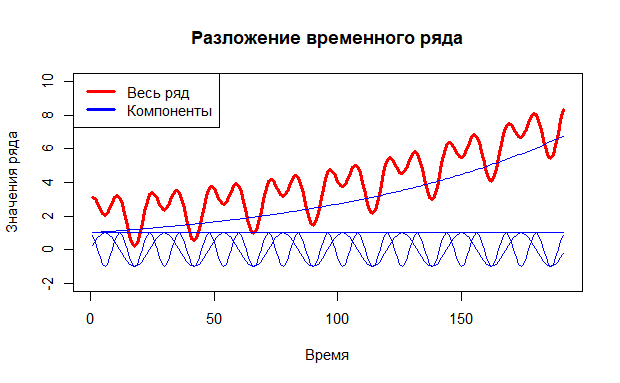
\includegraphics[width=0.8\textwidth]{img/trend inseparability example/all.png}
% %	\caption{Правильное разложение ряда $\TS = \TS_c + \TS_e + \TS_{\cos} + \TS_{\sin}$}
% %	\label{fig:c_e_cos}
% %\end{figure}
% %
% %\begin{figure}[H]
% %	\centering
% %	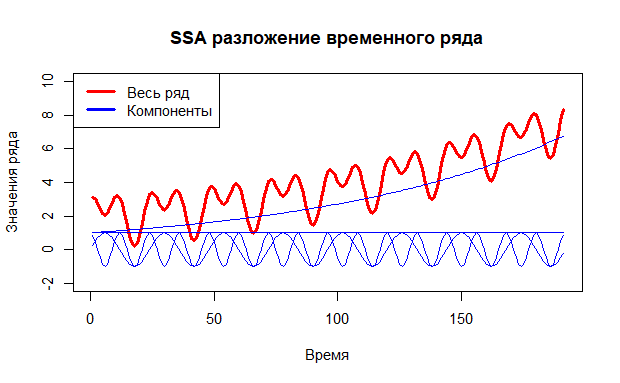
\includegraphics[width=0.8\textwidth]{img/trend inseparability example/ssa.png}
% %	\caption{Разложение ряда $\TS = \TS_c + \TS_e + \TS_{\cos} + \TS_{\sin}$ методом $\SSA$}
% %	\label{fig:c_e_cos_ssa}
% %\end{figure}
% %
% %Метод $\SSA$ разделил правильно все компоненты друг от друга.
% %
% %\begin{figure}[H]
% %	\centering
% %	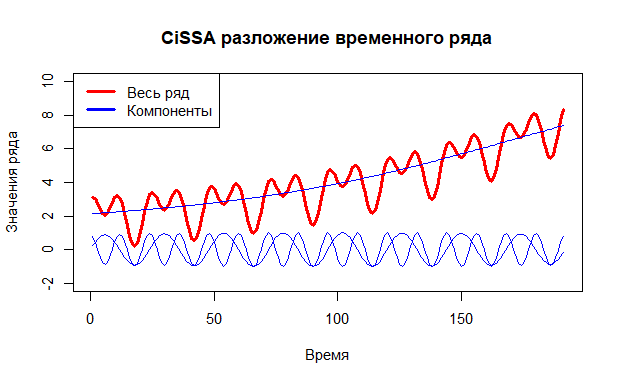
\includegraphics[width=0.8\textwidth]{img/trend inseparability example/cissa.png}
% %	\caption{Разложение ряда $\TS = \TS_c + \TS_e + \TS_{\cos} + \TS_{\sin}$ методом $\CISSA$}
% %	\label{fig:c_e_cos_cissa}
% %\end{figure}
% %
% %В случае $\CISSA$ получилось так, что экспонента и константа смешались в одну компоненту, одни и те же низкие частоты отвечают за них одновременно, поскольку они не являются периодиками.
% %
% %% latex table generated in R 4.2.2 by xtable 1.8-4 package
% %% Wed Jun 12 06:57:37 2024
% %\begin{table}[H]
% %	\centering
% %	\begin{tabular}{l|lll|llll}
% %		\hline
% %		Метод/Компонента & $\TS_e$ & $\TS_c$ & $\TS_c + \TS_e$ & $\TS_{\sin}$ & $\TS_{\cos}$ \\ 
% %		\hline
% %		SSA & 2.2e-25 & 2.2e-25 & 4.2e-28 &3.8e-29 & 1.6e-29 \\ 
% %		CiSSA &none & none & 3.5e-02 & 1.4e-04 & 1.9e-03 \\ 
% %		\hline
% %	\end{tabular}
% %	\caption{MSE разложений ряда $\TS = \TS_c + \TS_e + \TS_{\cos} + \TS_{\sin}$ методов $\SSA$ и \CISSA} 
% %	\label{tab:errs}
% %\end{table}
% %
% %Таблица \ref{tab:errs} и рисунки \ref{fig:c_e_cos_ssa}, \ref{fig:c_e_cos_cissa} показывают, что метод $\SSA$ справился лучше в сравнении с $\CISSA$, причем как по разделимости, так и по ошибке. В алгоритме $\CISSA$ трендовая составляющая также смешалась с сезонной, поэтому увеличилась ошибка при косинусе. Стоит отметить, что в данном примере использовался алгоритм улучшения разделимости EOSSA \cite{golyandina2023intelligent} для метода $\SSA$. Без него не получились бы такие результаты.
% %
% %Или же, если заменить $\TS_{e}$ на $\TS_{e \cdot \cos}$, то есть теперь ряд $\TS = \TS_c + \TS_{e \cdot \cos} + \TS_{\cos} + \TS_{\sin} = 1 + e^{\frac{x}{100}} \cos(\frac{2\pi}{48} x) + \cos(\frac{2\pi}{12} x) + \sin(\frac{2\pi}{24} x)$, то получится следующая таблица ошибок:
% %\begin{table}[H]
% %	\centering
% %	\begin{tabular}{l|lllllll}
% %		\hline
% %		Метод/Компонента & $\TS_{e \cdot \cos}$ & $\TS_{\sin}$ & $\TS_{\cos}$ \\ 
% %		\hline
% %		SSA & 4.7e-29 & 1.1e-29 & 8.4e-30 \\ 
% %		CiSSA  &3.2e-02 & 2.6e-04 & 5.8e-03 \\ 
% %		\hline
% %	\end{tabular}
% %	\caption{MSE разложений ряда $\TS = \TS_c + \TS_{e \cdot \cos} + \TS_{\cos} + \TS_{\sin}$ методов $\SSA$ и \CISSA} 
% %	\label{tab:errs_exp_cos}
% %\end{table}
% %
% %Таким образом, таблица \ref{tab:errs_exp_cos} показывает тот же недостаток у метода $\CISSA$, что и таблица \ref{tab:errs}.


% \subsection{Выделение тренда}


% % \begin{table}[H]
% % 	\caption{MSE разложений ряда $\TS = \TS_{c} + \TS_e + \TS_{\sin} + \TS_{\cos}$}
% % 	\centering
% % 	\begin{tabular}{l|l|cccc}
% % 		\hline
% % 		Метод              & Параметры            & $\operatorname{MSE}(\TS_{c} + \TS_e)$ & $\operatorname{MSE}(\TS_{\sin})$ & $\operatorname{MSE}(\TS_{\cos})$ & $\operatorname{MSE}(\TS)$ \\
% % 		\hline
% % 		SSA                & $L = 96, K = 96 $    & 6.1e-05                               & 8.9e-07                          & 5.2e-05                          & 2.1e-28                   \\
% % 		SSA                & $L = 96, K = 97 $    & 7.3e-05                               & 4.2e-06                          & 6.2e-05                          & 1.1e-27                   \\
% % 		\hline
% % 		Fourier            & $N = 96 \cdot 2$     & 1.1e-01                               & 6.1e-04                          & 6.8e-03                          & 1.1e-01                   \\
% % 		Fourier            & $N = 96 \cdot 2 - 1$ & 1.2e-01                               & 1.9e-02                          & 2.2e-02                          & 1.0e-01                   \\
% % 		\hline
% % 		Fourier extended   & $N = 96 \cdot 2$     & 1.4e-03                               & 1.3e-03                          & 8.4e-03                          & 9.6e-03                   \\
% % 		Fourier extended   & $N = 96 \cdot 2 - 1$ & 2.7e-03                               & 3.1e-04                          & 3.1e-03                          & 5.9e-03                   \\
% % 		\hline
% % 		CiSSA              & $L = 96$             & 5.3e-02                               & 1.6e-05                          & 4.9e-04                          & 4.4e-02                   \\
% % 		CiSSA              & $L = 97$             & 7.6e-02                               & 4.1e-02                          & 1.4e-02                          & 1.1e-01                   \\
% % 		\hline
% % 		CiSSA extended     & $L = 96$             & 5.0e-04                               & 2.1e-04                          & 1.1e-03                          & 6.0e-04                   \\
% % 		CiSSA extended     & $L = 97$             & 5.8e-04                               & 1.3e-02                          & 2.0e-03                          & 1.4e-02                   \\
% % 		\hline
% % 		SSA EOSSA, $r = 6$ & $L = 96, K = 96 $    & 1.7e-28                               & 1.6e-29                          & 8.7e-30                          & 1.6e-28                   \\
% % 		SSA EOSSA, $r = 6$ & $L = 96, K = 97 $    & 1.0e-27                               & 2.3e-29                          & 9.7e-30                          & 9.5e-28                   \\
% % 		\hline
% % 	\end{tabular}
% % 	\label{tab:errs_fourier_cissa_trend}
% % \end{table}



% \subsection{Отделение сигнала от шума}

% %НАПИСАТЬ РЕЗУЛЬТАТЫ ПРЕДЫДУЩИХ ПРИМЕРОВ С ШУМОМ. СДЕЛАТЬ ВЫВОДЫ.

% Рассмотрим влияние шума на результаты разделимости предыдущих примеров.

% \textbf{\large{Пример.}} Вернемся к примеру из секции \ref{subsubsec:exact} и добавим к нему шум: $\TS = \TS_{\sin} + \TS_{\cos} + \TS_{\mathrm{noise}} = \sin{\frac{2\pi}{12}n} + \frac{1}{2}\cos{\frac{2\pi}{3}n} + \varepsilon_n$, где $\varepsilon_n \sim \mathrm N(0, 0.1^2)$.
% Кроме того, для всех алгоритмов кроме базового $\SSA$ выделялись периодические компоненты по диапазонам $\left(\omega \pm \Delta \right)$, где $\Delta = \frac{1}{N+1}$, $\omega = \frac{1}{12}, \frac{1}{3}$.
% Проводилось $100$ тестов, в таблице \ref{tab:errs_fourier_cissa_sin_cos_noised} указаны средние значения ошибки для одних и тех же реализаций шума.
% \begin{table}[H]
% 	\caption{MSE разложений ряда $\TS = \TS_{\sin} + \TS_{\cos} +\TS_{\mathrm{noise}}$ }
% 	\centering
% 	\begin{tabular}{l|l|ccc}
% 		\hline
% 		Метод              & Параметры            & $\operatorname{MSE}(\TS_{\sin})$ & $\operatorname{MSE}(\TS_{\cos})$ & $\operatorname{MSE}(\TS)$ \\
% 		\hline
% 		SSA                & $L = 96, K = 96 $    & 2.9e-04                          & 3.1e-04                          & 5.9e-04                   \\
% 		SSA                & $L = 96, K = 97 $    & 2.9e-04                          & 3.1e-04                          & 5.9e-04                   \\
% 		\hline
% 		Fourier            & $N = 96 \cdot 2$     & 1.0e-04                          & 1.1e-04                          & 2.2e-04                   \\
% 		Fourier            & $N = 96 \cdot 2 - 1$ & 1.8e-02                          & 7.6e-03                          & 2.6e-02                   \\
% 		\hline
% 		Fourier extended   & $N = 96 \cdot 2$     & 1.2e-03                          & 3.9e-03                          & 5.1e-03                   \\
% 		Fourier extended   & $N = 96 \cdot 2 - 1$ & 1.2e-03                          & 8.4e-04                          & 2.0e-03                   \\
% 		\hline
% 		CiSSA              & $L = 96$             & 1.6e-04                          & 1.8e-04                          & 3.4e-04                   \\
% 		CiSSA              & $L = 97$             & 4.1e-02                          & 1.2e-02                          & 5.2e-02                   \\
% 		\hline
% 		CiSSA extended     & $L = 96$             & 6.6e-04                          & 1.9e-03                          & 2.5e-03                   \\
% 		CiSSA extended     & $L = 97$             & 1.4e-02                          & 3.0e-03                          & 1.7e-02                   \\
% 		\hline
% 		SSA EOSSA, $r = 4$ & $L = 96, K = 96 $    & 2.9e-04                          & 3.1e-04                          & 5.9e-04                   \\
% 		SSA EOSSA, $r = 4$ & $L = 96, K = 97 $    & 2.9e-04                          & 3.0e-04                          & 5.9e-04                   \\
% 		\hline
% 	\end{tabular}
% 	\label{tab:errs_fourier_cissa_sin_cos_noised}
% \end{table}


% % Sun Feb 16 18:11:24 2025
% %\begin{table}[ht]
% %	\centering
% %	\begin{tabular}{llll}
% %		\hline
% %		Метод & sin\_err & cos\_err & all\_err \\ 
% %		\hline
% %		SSA & 2.9e-04 & 3.1e-04 & 5.9e-04 \\ 
% %		SSA EOSSA & 2.9e-04 & 3.1e-04 & 5.9e-04 \\ 
% %		Fourier & 1.0e-04 & 1.1e-04 & 2.2e-04 \\ 
% %		CiSSA & 1.6e-04 & 1.8e-04 & 3.4e-04 \\ 
% %		CiSSA extended & 6.6e-04 & 1.9e-03 & 2.5e-03 \\ 
% %		Fourier extended & 1.2e-03 & 3.9e-03 & 5.1e-03 \\ 
% %		\hline
% %	\end{tabular}
% %	\caption{Example Table} 
% %\end{table}

% По таблице \ref{tab:errs_fourier_cissa_sin_cos_noised} видно, что зашумление ряда сильно повлияло на ошибку, теперь она не является машинным нулем ни для одного из методов. Также был проведен парный t-критерий для зависимых выборок с целью проверки гипотезы о равенстве средних значений ошибки для каждой компоненты, попарно для всех методов. В качестве нулевой гипотезы ($H_0$) предполагалось, что средние значения двух сравниваемых выборок равны. Критический уровень значимости был установлен на уровне $\alpha = 0.05$.
% Результаты анализа показали, что во всех случаях, кроме сравнения $\SSA$ и $\SSA$ с EOSSA, $p$-значение оказалось меньше 0.05, что позволяет отвергнуть нулевую гипотезу.

% \textbf{\large{Пример.}} Теперь вновь добавим трендовую составляющую к ряду: $\TS = \TS_{c} + \TS_e + \TS_{\sin} + \TS_{\cos} + \TS_{\mathrm{noise}} = 1 + e^{\frac{x}{100}} + \sin{\frac{2\pi}{12}x} + \frac{1}{2}\cos{\frac{2\pi}{3}x} + \varepsilon_n$, где $\varepsilon_n \sim \mathrm N(0, 0.1^2)$. Кроме того, для всех алгоритмов кроме базового $\SSA$ выделялись периодические компоненты по диапазонам $\left(\omega \pm \Delta \right)$, где $\Delta = \frac{1}{N+1}$, $\omega = \frac{1}{12}, \frac{1}{3}$, а непериодичность соответствовала диапазону частот $\left[0, \frac{1}{24} \right)$. Проводилось $100$ тестов, в таблице \ref{tab:errs_fourier_cissa_trend_noised} указаны средние значения ошибки для одних и тех же реализаций шума.

% \begin{table}[H]
% 	\caption{MSE разложений ряда $\TS = \TS_{\sin} + \TS_{\cos} + \TS_{c} + \TS_e+\TS_{\mathrm{noise}}$ методов}
% 	\centering
% 	\begin{tabular}{l|l|cccc}
% 		\hline
% 		Метод              & Параметры          & $\operatorname{MSE}(\TS_{c} + \TS_e)$ & $\operatorname{MSE}(\TS_{\sin})$ & $\operatorname{MSE}(\TS_{\cos})$ & $\operatorname{MSE}(\TS)$ \\
% 		\hline
% 		SSA                & $L = 96, K = 96 $  & 5.2e-03                               & 2.9e-04                          & 3.6e-04                          & 5.2e-03                   \\
% 		SSA                & $L = 96, K = 97 $  &
% 		5.5e-03            & 2.9e-04            & 3.7e-04                               & 5.3e-03                                                                                         \\
% 		\hline
% 		Fourier            & $N = 96 \cdot 2$   & 1.2e-01                               & 6.9e-04                          & 7.2e-03                          & 1.1e-01                   \\
% 		Fourier            & $N = 96 \cdot 2-1$ &
% 		1.2e-01            & 1.9e-02            & 2.2e-02                               & 1.0e-01                                                                                         \\
% 		\hline
% 		Fourier extended   & $N = 96 \cdot 2$   & 3.0e-03                               & 1.9e-03                          & 9.6e-03                          & 1.2e-02                   \\
% 		Fourier extended   & $N = 96 \cdot 2-1$ &
% 		4.7e-03            & 8.6e-04            & 3.0e-03                               & 7.8e-03                                                                                         \\
% 		\hline
% 		CiSSA              & $L = 96$           & 5.5e-02                               & 1.7e-04                          & 7.0e-04                          & 4.6e-02                   \\
% 		CiSSA              & $L = 97$           &
% 		7.7e-02            & 4.1e-02            & 1.4e-02                               & 1.1e-01                                                                                         \\
% 		\hline
% 		CiSSA extended     & $L = 96$           & 2.7e-03                               & 6.8e-04                          & 2.1e-03                          & 3.1e-03                   \\
% 		CiSSA extended     & $L = 97$           &
% 		2.7e-03            & 1.4e-02            & 3.3e-03                               & 1.7e-02                                                                                         \\
% 		\hline
% 		SSA EOSSA, $r = 6$ & $L = 96, K = 96 $  & 9.5e-04                               & 2.9e-04                          & 3.1e-04                          & 1.5e-03                   \\
% 		SSA EOSSA, $r = 6$ & $L = 96, K = 97 $  &
% 		9.3e-04            & 2.9e-04            & 3.1e-04                               & 1.5e-03                                                                                         \\
% 		\hline
% 	\end{tabular}
% 	\label{tab:errs_fourier_cissa_trend_noised}
% \end{table}


% Как видно из таблицы \ref{tab:errs_fourier_cissa_trend_noised}, разделения ухудшились, однако $\SSA$ с улучшением разделимости EOSSA отработал лучше всех, а хуже всех показали себя алгоритмы Фурье. Также был проведен был проведён двухвыборочный t-критерий для зависимых выборок с целью проверки гипотезы о равенстве средних значений ошибки для каждой компоненты, попарно для всех методов. В качестве нулевой гипотезы ($H_0$) предполагалось, что средние значения двух сравниваемых выборок равны. Критический уровень значимости был установлен на уровне $\alpha = 0.05$.
% Результаты анализа показали, что во всех случаях, кроме сравнения синуса для базового $\SSA$ и $\SSA$ с EOSSA, а также синуса для Фурье и расширенного $\CISSA$, $p$-значение оказалось меньше $0.05$, что позволяет отвергнуть нулевую гипотезу.

% Таким образом, можно сделать вывод, что алгоритмы отделяют сигнал от шума примерно одинаково, когда ряд состоит из периодик и параметры правильно подобраны. Результаты не сильно изменяются для базового $\SSA$ и $\SSA$ с EOSSA. Для $\CISSA$ и Фурье результаты ухудшаются. С добавлением трендовой составляющей ситуация меняется: для $\SSA$ результаты практически не ухудшаются, $\CISSA$ с расширением показывает себя немного хуже $\SSA$, остальные алгоритмы выдают значения ошибки на порядки большие.

\subsection{Разделение трендовых составляющих между собой}
\label{subsubsec:nonperiodic}

Как удалось выяснить, все рассматриваемые алгоритмы могут выделять трендовую составляющую из ряда. Однако лишь $\SSA$ способен различить между собой две непериодических компоненты. Про скорость асимптотической разделимости для $\SSA$ можно подробнее узнать в книге \cite{golyandina2001analysis}. Методы $\CISSA$ и Фурье никаким образом не смогут отличить две непериодики между друг другом, поскольку они объединяют компоненты только по частотам. А двум непериодикам соответствуют одинаковые (низкие) наборы частот.


\subsection{Преимущества и недостатки методов SSA, Фурье и CiSSA}
%ДОБАВИТЬ НЕДОСТАЮЩИЕ ПРИМЕРЫ ПО СТОЛБЦАМ, СКАЗАТЬ, КАКИЕ СТОЛБЦЫ УЖЕ С ПРИМЕРАМИ (ИЗ ПРЕДЫДУЩИХ СЕКЦИЙ), СДЕЛАТЬ МИНИ ВЫВОДЫ


Из ранее рассмотренных примеров и теоретических результатов можно сделать следующие выводы:

\begin{itemize}
	\item Для $\CISSA$ условия точной разделимости слабее, чем для $\SSA$ (\ref{subsec:cissa_exact});
	\item Процедура расширения ряда улучшает выделение тренда для $\CISSA$ и $\FOURIER$, однако $\SSA$ справляется с этой задачей лучше (\ref{example:cissa_trend_noise});
	\item $\CISSA$ показывает результаты лучше, чем обычный $\FOURIER$ (\ref{subsec:cissa_L_choice});
	\item За счет фиксированного базиса в $\CISSA$ возникают такие проблемы, как утечка спектра и трудность при выборе диапазонов частот для объединения (\ref{subsec:cissa_fixed_basis_problems});
	\item Базовый $\SSA$ численно не хуже, чем $\CISSA$, а шум выделяет лучше (\ref{subsec:cissa_examples_without_noise}, \ref{subsec:cissa_examples_with_noise});
	\item $\EOSSA$ исправляет недостатки базового $\SSA$, значительно улучшая результаты (\ref{subsec:cissa_examples_without_noise}, \ref{subsec:cissa_examples_with_noise}). 
\end{itemize}

% Для наглядного отображения преимуществ каждого из этих методов составлены похожие по смыслу таблицы \ref{tab:advantages_ssa_cissa} и \ref{tab:advantages_fourier}, где строки соответствуют методам, а столбцы --- условиям (особым видам компонент ряда). Разделение на две таблицы объяснимо тем, что методам $\SSA$ и $\CISSA$ важно, какие $L$ и  $K$ выбраны у ряда, в то время как разложение Фурье волнует только $N$. На пересечении строк и столбцов указан знак, показывающий, достигается ли разделение компоненты: плюс (+) обозначает точное выполнение, знак стремления указывает на асимптотическое выполнение, а минус (–) --- на отсутствие разделимости.

% Обозначения:
% \begin{itemize}
% 	\item $\cos$ --- в ряде присутствуют только периодические компоненты вида $A\cos(2\pi \omega x + \varphi)$;
% 	\item $\TS_{\mathrm{np}1}$ --- одна непериодическая компонента в ряде, остальные имеют период;
% 	\item $\TS_{\mathrm{np}}$ --- несколько непериодических компонент в ряде, остальные имеют период, интересует разделение между
% 	      непериодическими компонентами;
% 	\item group --- автоматическая группировка по заданным частотам.
% \end{itemize}


% \begin{table}[H]
% 	\caption{Преимущества и недостатки методов $\SSA$, $\CISSA$.}
% 	\centering
% 	\begin{center}
% 		\begin{tabular}{l|cccccccc}
% 			\hline
% 			Метод/Условие  & $\cos$,             & $\cos$,                & $\cos$,                 & $\TS_{\mathrm{np1}}$ & $\TS_{\mathrm{np}}$ & group \\
% 			               & $Lw \in \mathbb N$, & $Lw\in \mathbb N$,     & $Lw \not\in \mathbb N$, &                                                    \\
% 			               & $Kw\in \mathbb N$   & $Kw \not\in \mathbb N$ & $Kw \not\in \mathbb N$  &                                                    \\
% 			\hline
% 			SSA            & $+$                 & $\to$                  & $\to$                   & $\to$                & $\to$               & $-$   \\
% 			SSA EOSSA      & $+$                 & $\to$                  & $\to$                   & $\to$                & $\to$               & $+$   \\
% 			CiSSA          & $+$                 & $+$                    & $\to$                   & $-$                  & $-$                 & $+$   \\
% 			CiSSA extended & $+$                 & $+$                    & $\to$                   & $\to$                & $-$                 & $+$   \\
% 			\hline
% 		\end{tabular}
% 	\end{center}
% 	\label{tab:advantages_ssa_cissa}
% \end{table}

% \begin{table}[H]
% 	\caption{Преимущества и недостатки методов Fourier.}
% 	\centering
% 	\begin{center}
% 		\begin{tabular}{l|cccccccc}
% 			\hline
% 			Метод/Условие    & cos,               & cos,                    & $\TS_{\mathrm{np1}}$ & $\TS_{\mathrm{np}}$ & group \\
% 			                 & $Nw \in \mathbb N$ & $Nw \not \in \mathbb N$                                                      \\
% 			\hline
% 			Fourier          & $+$                & $\to$                   & $-$                  & $-$                 & $+$   \\
% 			Fourier extended & $+$                & $\to$                   & $\to$                & $-$                 & $+$   \\
% 			\hline
% 		\end{tabular}
% 	\end{center}
% 	\label{tab:advantages_fourier}
% \end{table}



% Большинство ситуаций из таблицы \ref{tab:advantages_ssa_cissa} и  \ref{tab:advantages_fourier} уже были разобраны в предыдущих разделах. Так, столбцы, связанные с $\cos$, были разобраны в разделах \ref{subsubsec:exact} и \ref{subsubsec:asymp}. Ситуация с одной непериодической компонентой разобрана в \ref{subsubsec:trend}, а с отделением нескольких непериодик в \ref{subsubsec:nonperiodic}. Автоматическая группировка компонент по заранее заданным частотам в \ref{subsubsec:autogroup}.

% Анализ полученных результатов показывает, что $\CISSA$ превосходит разложение Фурье как с расширением ряда, так и без него, во всех случаях, когда интересующие частоты совпадают с частотной решеткой алгоритмов. Если же частоты не совпадают, разложение Фурье может дать лучший результат благодаря более детальному разбиению частот. Кроме того, $\SSA$ с улучшением разделимости EOSSA продемонстрировал более высокую эффективность по сравнению со всеми ранее рассматриваемыми алгоритмами.



\subsection{Демонстрация работы алгоритмов на реальных данных}
\label{subsubsec:real_dataZz}
%УБРАТЬ ПРО АВТОМАТИЧЕСКУЮ ГРУППИРОВКУ, ОСТАВИТЬ ТОЛЬКО РЕАЛЬНЫЙ ПРИМЕР

Теперь рассмотрим реальные данные --- месячные ряды промышленного производства (Industrial Production, IP), index $2010 = 100$, в США. Данные промышленного производства полезны, поскольку оно указывается в определении рецессии Национальным бюро экономических исследований (NBER), как один из четырех ежемесячных рядов индикаторов, которые необходимо проверять при анализе делового цикла. Выборка охватывает период с января 1970 года по сентябрь 2014 года, поэтому размер выборки составляет $N = 537$. Источником данных является база данных IMF. Эти показатели демонстрируют различные тенденции, сезонность и цикличность (периодические компоненты, которые соответствуют циклам бизнеса). Данные IP также рассматривались в статье \cite{bogalo2020}.
Применим как $\CISSA$ с расширением ряда, так и $\SSA$ с автоматическим определением частот и улучшениями разделимости EOSSA и FOSSA с параметром $r = 30$ по следующим группам:
\begin{enumerate}
	\item Трендовой составляющей должны отвечать низкие частоты, поэтому диапазон: $\left[0, \frac{1}{192}\right]$;
	\item Циклы бизнеса по диапазонам: $\left[\frac{2}{192}, \frac{10}{192}\right]$;
	\item Сезонность по частотам $\omega_k = 1/12, 1/6, 1/4, 1/3, 5/12, 1/2$;
\end{enumerate}
На основе предыдущих требований взято $L = 192$.

\begin{figure}[H]
	\centering
	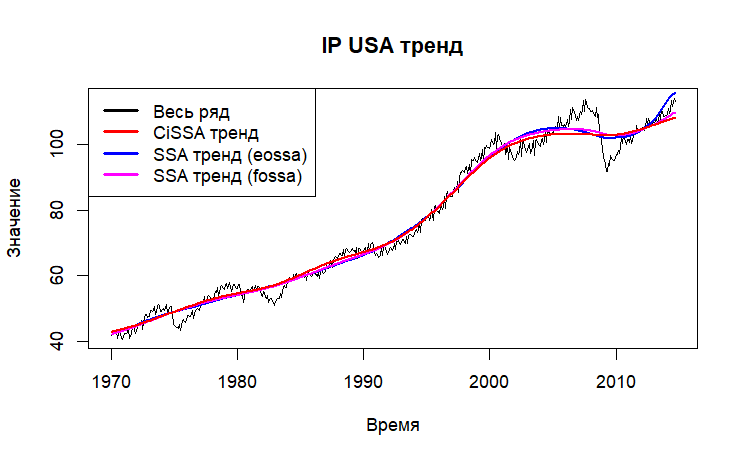
\includegraphics[width=0.8\textwidth]{img/trend inseparability example/IP_trend.png}
	\caption{Трендовая составляющая данных IP USA.}
	\label{fig:IP_trend}
\end{figure}

При применении FOSSA улучшения разделимости алгоритм $\SSA$ выделяет тренд довольно похоже с $\CISSA$. Весь график $\SSA$ тренд EOSSA выглядит более изогнутым при визуальном сравнении с остальными.

\begin{figure}[H]
	\centering
	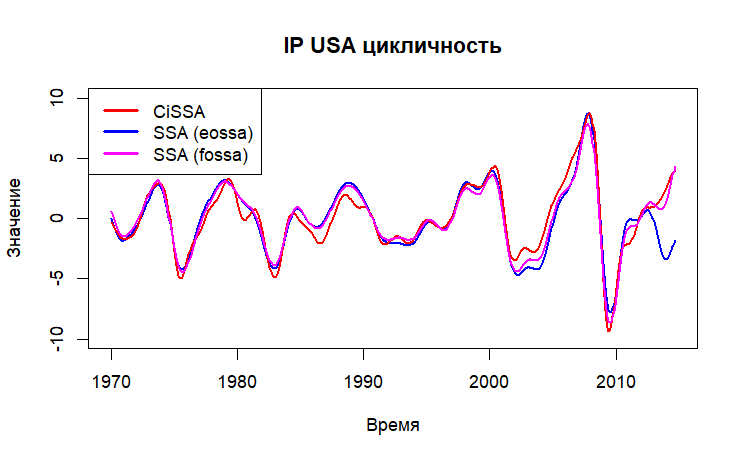
\includegraphics[width=0.8\textwidth]{img/trend inseparability example/IP_cycle.png}
	\caption{Циклическая составляющая данных IP USA.}
	\label{fig:IP_cycle}
\end{figure}

Аналогичная тренду ситуация происходит с цикличностью. В случае EOSSA правый хвост (значения ряда после 2010-ого года) смешался между цикличностью и трендом.

\begin{figure}[H]
	\centering
	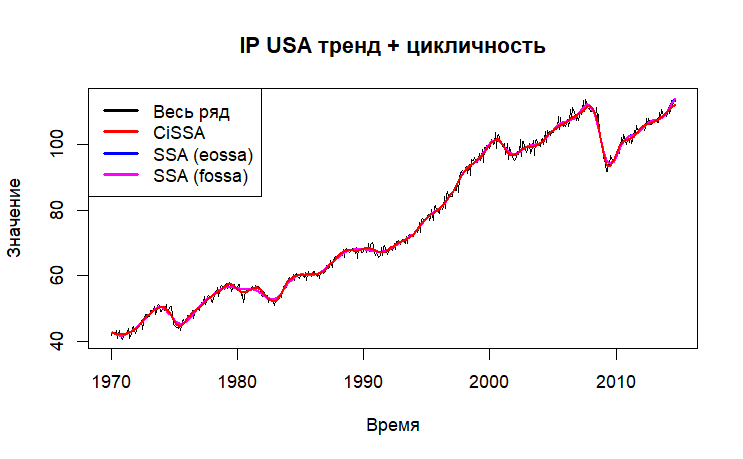
\includegraphics[width=0.8\textwidth]{img/trend inseparability example/IP_trend_sycle.png}
	\caption{Объединение тренда и цикличности IP USA.}
	\label{fig:IP_trend_sycle}
\end{figure}

Как видно из графика \ref{fig:IP_trend_sycle}, объединив тренд и цикличность получаем одинаковые результаты для всех рассматриваемых алгоритмов.

\begin{figure}[H]
	\centering
	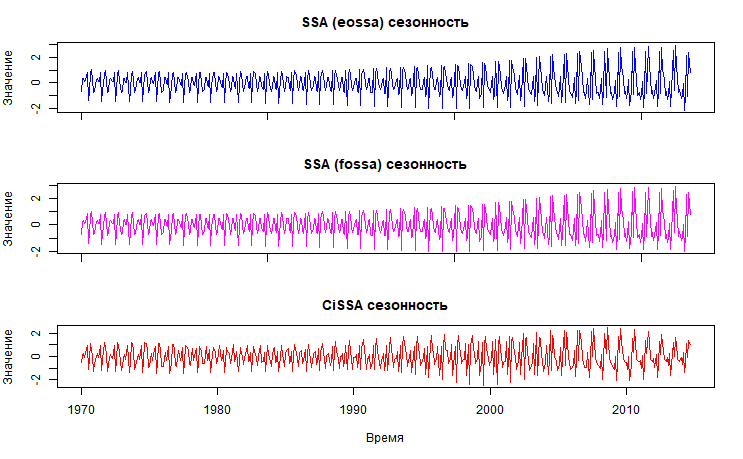
\includegraphics[width=0.8\textwidth]{img/trend inseparability example/IP_sesonal.jpg}
	\caption{Сезонная составляющая данных IP USA.}
	\label{fig:IP_sesonal}
\end{figure}

Сезонность выглядит схоже для EOSSA и FOSSA. Несколько иначе для $\CISSA$.

%\begin{figure}[H]
%	\centering
%	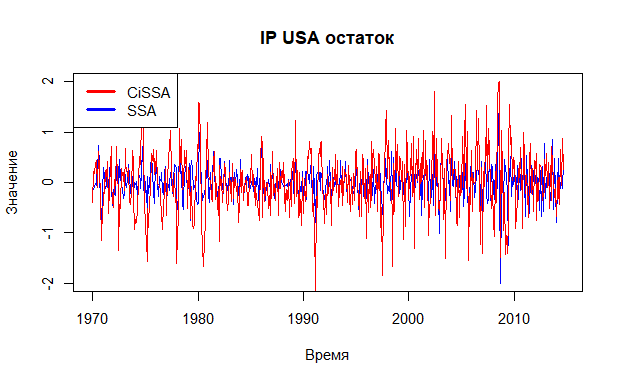
\includegraphics[width=0.8\textwidth]{img/trend inseparability example/IP_residuals.png}
%	\caption{Шум данных IP USA}
%	\label{fig:IP_residuals}
%\end{figure}
Шум же является нормальным во всех случаях.

% \begin{figure}[H]
% 	\centering
% 	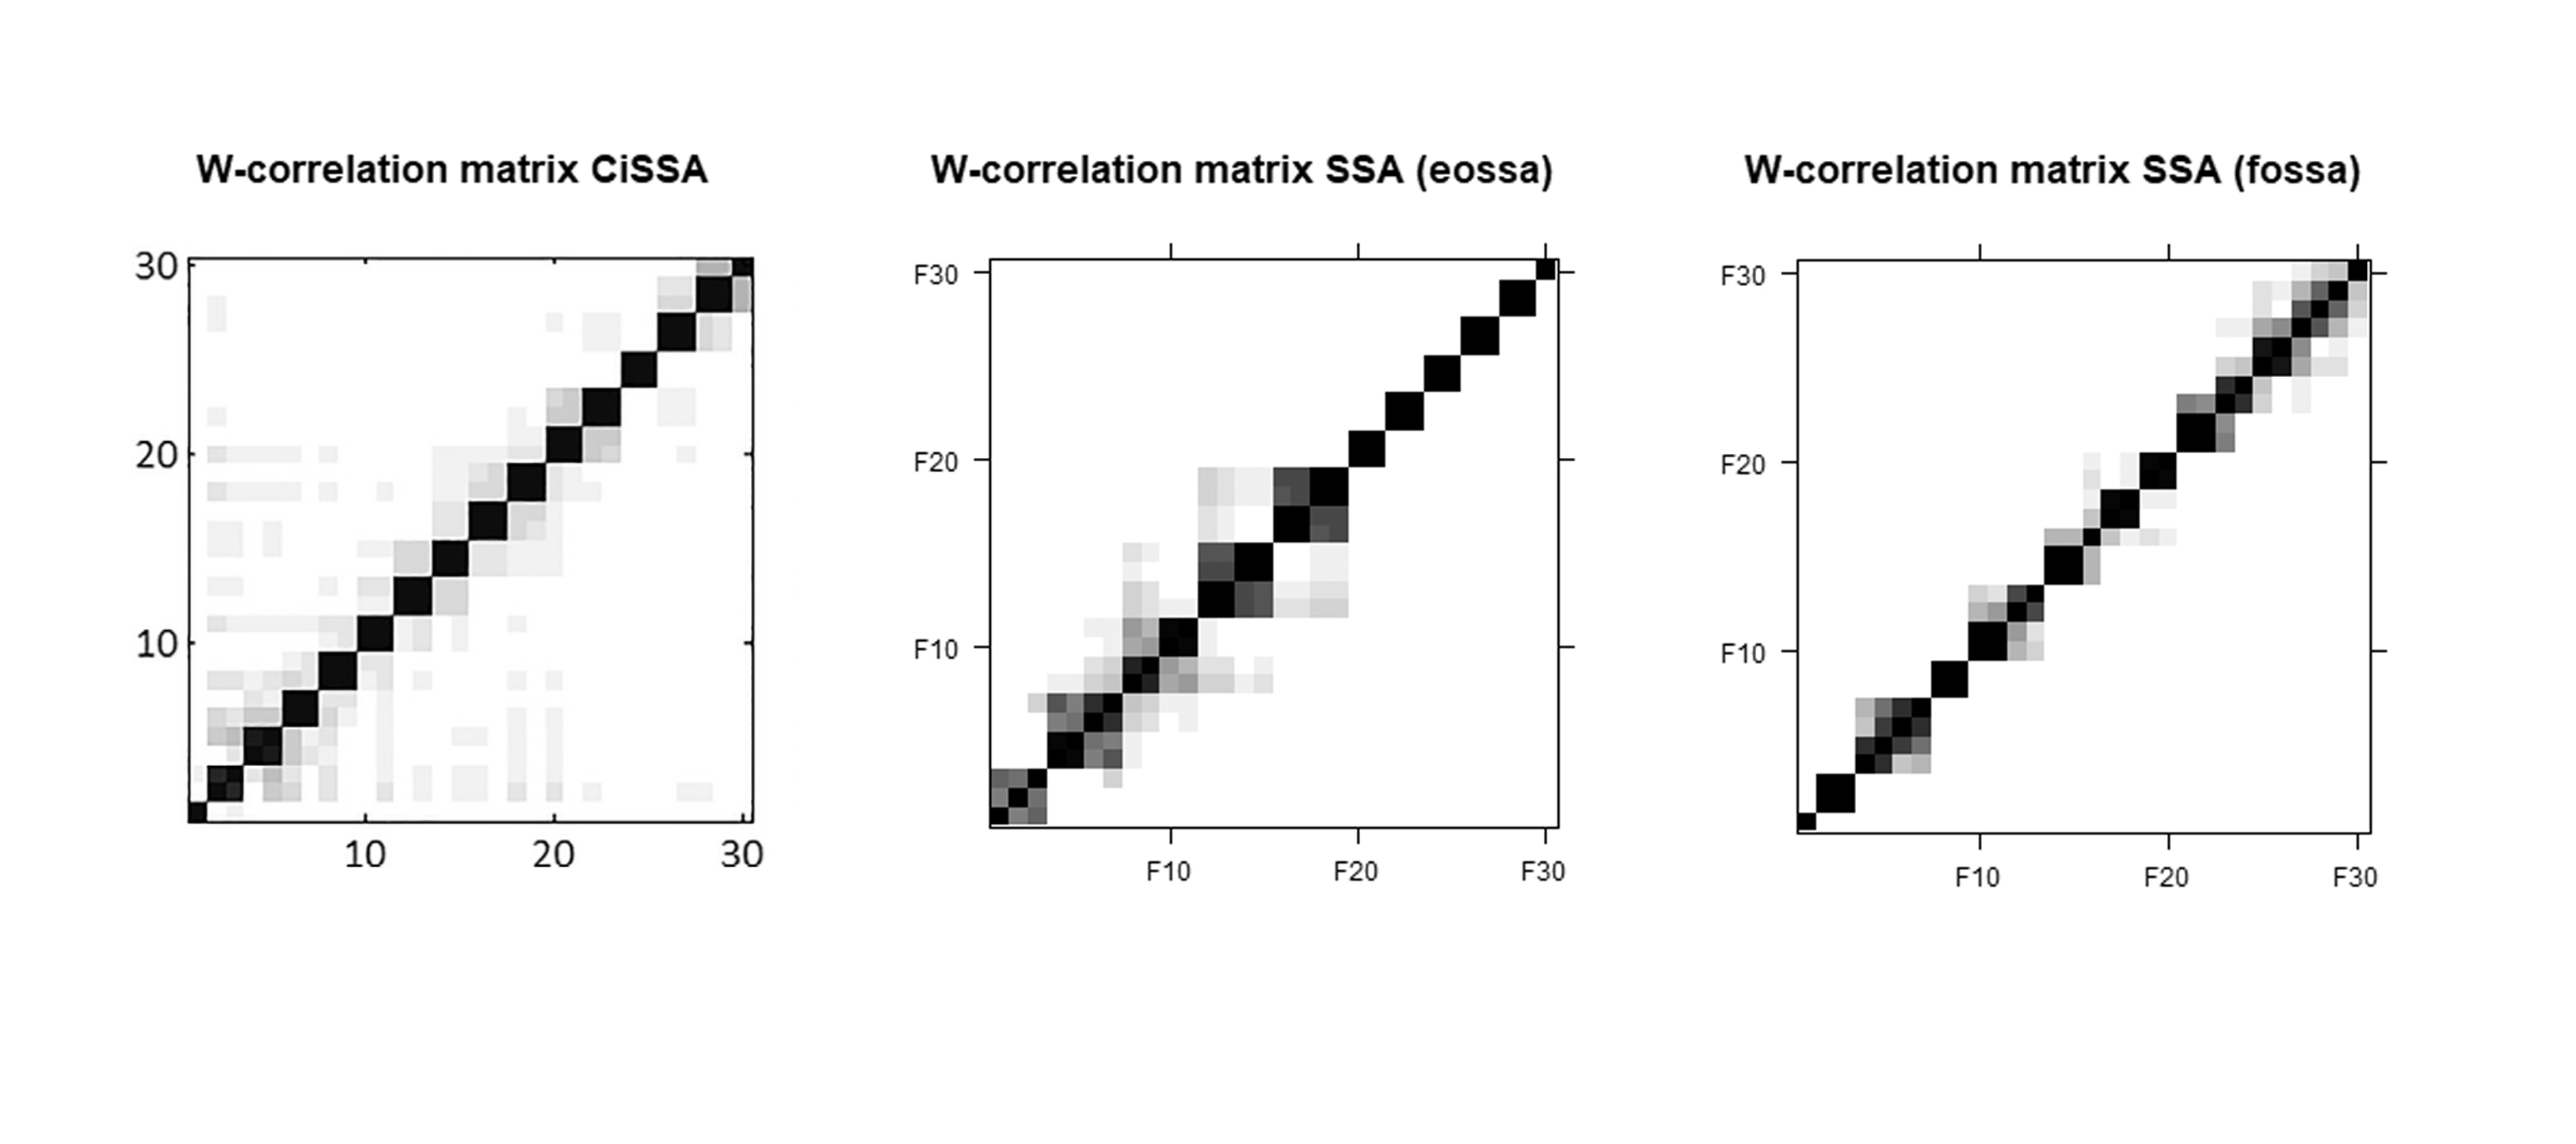
\includegraphics[width=0.8\textwidth]{img/trend inseparability example/W-corr.jpg}
% 	\caption{Матрицы корреляций IP USA}
% 	\label{fig:W-corr}
% \end{figure}
% %TODO: по pdf
% По матрицам корреляции заметно, что при использовании $\SSA$ с улучшением разделимости EOSSA, смешиваются первые по значимости компоненты ряда (они и являются трендовыми и циклическими).

%\textbf{ОТСЕБЯТИНА}
%Тренд наиболее гибко и лучше отделяется при применении SSA, цикличность отделилась одинаково в обоих случаях, сезонность выглядит куда приличнее при применении CiSSA. Плюс, приходится подбирать параметры разложения в SSA. В CiSSA вообще ничего не надо делать, просто вкинул, отработало замечательно. 


Таким образом, получились довольно похожие результаты в выделении тренда и цикличности при использовании $\SSA$ с FOSSA и $\CISSA$. Несколько иные результаты при $\SSA$ с EOSSA.

\newpage





% \section{Многомерные варианты базового SSA}

% \label{sec:multidimensional_ssa}

% Временные ряды могут быть не только одномерными, но и многомерными, то есть представлять собой наборы связанных наблюдений. В данной работе рассматриваются две модификации базового $\SSA$:
% $\MSSA$ и $\DSSA$.

% Под многомерным временным рядом будем понимать систему $s$ одномерных временных рядов $\TS = (\TS^{(1)}, \ldots, \TS^{(s)})$, где каждый ряд $\TS^{(p)} = (x_1^{(p)}, \ldots, x_{N_p}^{(p)})$ представляет собой последовательность числовых значений.

% Под двумерным рядом будем понимать прямоугольную матрицу $\TS = [x_{ij}] \in \mathbb{R}^{N_x \times N_y}$, содержащую наблюдения, упорядоченные по двум пространственным или иным измерениям (например, изображение).

% % Каждый из методов -- $\MSSA$ и $\DSSA$ -- использует свою стратегию формирования траекторной матрицы и, соответственно, имеет особенности в разложении, реконструкции и прогнозировании. Далее будут подробно рассмотрены обе эти модификации SSA, их алгоритмы, интерпретации и примеры применения.


% \subsection{MSSA}

% Рассмотрим многомерный временной ряд, то есть набор $\{\mathbb{X}^{(p)} = \left({x^{(p)}_{j}}\right) _{j=1}^{N_p}, \; p = 1, \ldots, s\}$ из $s$ временных рядов длины $N_p$, где $p = 1, \ldots, s$.

% Обозначим $\mathbb{X} = (\mathbb{X}^{(1)}, \ldots, \mathbb{X}^{(s)})$ как исходные данные для алгоритма $\MSSA$ \cite{ssa_with_R}. Общая схема алгоритма базового $\SSA$. Необходимо лишь определить оператор вложения $\EuScript{T}_{\text{\MSSA}}(\mathbb{X}) = \mathbf X$.

% \subsubsection*{Вложение}

% Пусть $L$ -- длина окна, $1 < L < \min(N_p, \; p = 1, \ldots, s)$. Для каждого временного ряда $\TS^{(p)}$ формируем $K_p = N_p - L + 1$ векторов $\mathbf{X}_j^{(p)} = (x_j^{(p)}, \ldots, x_{j+L-1}^{(p)})^T$, где $1 \leq j \leq K_p$. Обозначим $K = \sum_{p=1}^s K_p$. Траекторная матрица многомерного ряда $\TS$ — это матрица размера $L \times K$ следующего вида:

% \[
% 	\EuScript{T}_{\text{MSSA}}(\TS) = \mathbf{X} = [\mathbf{X}_1^{(1)} : \ldots : \mathbf{X}_{K_1}^{(1)} : \ldots : \mathbf{X}_1^{(s)} : \ldots : \mathbf{X}_{K_s}^{(s)}] = [\mathbf{X}^{(1)} : \ldots : \mathbf{X}^{(s)}],
% \]

% где $\mathbf{X}^{(p)} = \EuScript{T}_{\text{SSA}}(\TS^{(p)})$ — траекторная матрица одномерного ряда $\TS^{(p)}$. Таким образом, траекторная матрица системы временных рядов имеет блочно-ганкелеву структуру. Заметим, что

% \[
% 	\EuScript{T}^{-1}_{\text{MSSA}}(\mathbf{X}) = [\EuScript{T}^{-1}_{\text{SSA}}(\mathbf{X}^{(1)}) : \ldots : \EuScript{T}^{-1}_{\text{SSA}}(\mathbf{X}^{(s)})].
% \]



% \subsubsection*{Группировка}

% Аналогично базовому $\SSA$.

% \subsubsection*{Диагональное усреднение}

% Аналогично базовому $\SSA$ \eqref{eq:ssa_projector} определим оператор проектирования для $\MSSA$:

% \[
% 	\Pi_{\text{stacked } \mathcal{H}}(\mathbf{Y}) = [\Pi_{\mathcal{H}}(\mathbf{Y}^{(1)}) : \ldots : \Pi_{\mathcal{H}}(\mathbf{Y}^{(i)})]
% \]

% Тогда получаем восстановление с помощью $\EuScript{T}_{\text{MSSA}}^{-1} \circ \Pi_{\text{stacked }}$.




% \subsubsection{Комментарии}


% Собственные векторы $U_i$ из SVD траекторной матрицы $\mathrm{X} = \sum_i \sqrt{\lambda_i} U_i V_i^{\mathsf{T}}$ формируют общее базисное пространство для всех временных рядов. Векторы факторов $V_i$ содержат подкомпоненты $V_i^{(p)}$, соответствующие каждому ряду:

% \begin{equation*}
% 	V_i = \begin{pmatrix} V_i^{(1)} \\ \vdots \\ V_i^{(s)} \end{pmatrix},
% \end{equation*}

% где $V_i^{(p)} \in \mathbb{R}^{K_p}$ принадлежит строковому пространству $p$-го ряда. $U_i$ отражают общую структуру, $V_i^{(p)}$ — её проявление в отдельных рядах.


% Кроме того, $\MSSA$ позволяет вычленить дополнительную информацию про структуру рядов, рассматривая их совместно.



% \subsection{2d-ssa}

% $\DSSA$ -- это расширение базового $\SSA$ для двумерных массивов \cite{ssa_with_R} (например, изображений). Данные представляются в виде матрицы:
% \[
% 	\TS = (x_{ij})_{i,j=1}^{N_x, N_y}, \quad \text{где } N_x \times N_y \text{ — размер массива.}
% \]

% Параметрами метода являются размеры {окна} $(L_x, L_y)$, где $1 \leq L_x \leq N_x$, $1 \leq L_y \leq N_y$.

% \subsubsection*{Вложение}

% Как и в $\MSSA$, нужно определить лишь $\EuScript{T}_{\text{2D-SSA}}$

% \begin{enumerate}
% 	\item Из массива $\TS$ выделяются {все возможные подматрицы} размера $L_x \times L_y$ с помощью скользящего окна.
% 	\item Каждая подматрицы $\TS_{k,l}^{(L_x, L_y)}$ преобразуется в столбец: $\mathbf{X}_{k+(l-1)K_x} = \text{vec}(\TS_{k,l}^{(L_x, L_y)})$.
% 	\item Траекторная матрица строится как объединение этих столбцов:
% 	      \[
% 		      \EuScript{T}_{\text{2D-SSA}}(\TS) = \mathbf{X} = [\mathbf{X}_1 : \ldots : \mathbf{X}_{K_x K_y}].
% 	      \]
% \end{enumerate}

% Матрица $\mathbf{X}$ имеет {блочно-ганкелеву структуру}:
% \[
% 	\mathbf{X} =
% 	\begin{pmatrix}
% 		\mathbf{H}_1     & \mathbf{H}_2       & \ldots & \mathbf{H}_{K_y}   \\
% 		\mathbf{H}_2     & \mathbf{H}_3       & \ldots & \mathbf{H}_{K_y+1} \\
% 		\vdots           & \vdots             & \ddots & \vdots             \\
% 		\mathbf{H}_{L_y} & \mathbf{H}_{L_y+1} & \ldots & \mathbf{H}_{N_y}
% 	\end{pmatrix},
% \]
% где каждая $\mathbf{H}_j$ — ганкелевская матрица, построенная из столбцов $\TS$.

% \subsubsection*{Вложение}

% Аналогично базовому $\SSA$.

% \subsubsection*{Группировка}

% Аналогично базовому $\SSA$.

% \subsubsection*{Диагональное усреднение}

% Аналогично базовому $\SSA$, только восстановление производится по соответствующим ганкелевым блокам матрицы $\mathbf{X}$.

% \subsubsection{Комментарии}

% {Связь с $\MSSA$:} если $L_x = 1$ или $L_y = 1$, $\DSSA$ эквивалентен $\MSSA$ для временных рядов одинаковой длины. Поэтому его можно назвать обобщением $\MSSA$.

% Также при применении $\DSSA$ важен порядок следования строк и столбцов в $\TS$, в отличие от $\MSSA$.



% \newpage




\section{Сравнение FSSA, MSSA, 2d-SSA}

\label{sec:compare_fssa_ssa}

В оригинальной работе $\FSSA$ \cite{haghbin2019functionalsingularspectrumanalysis} рассматривалось сравнение алгоритма с dFPCA, $\MSSA$. Однако, $\DSSA$ в данном сравнении не было, хотя он может показать результаты лучше, чем $\MSSA$, за счет того, что в $\DSSA$ можно рассматривать зависимость по второй переменной.


\subsection{Численное сравнение}

Рассматриваются функциональные временные ряды длины $N=50, 100, 150$ и $200$, наблюдаемые в $M=100$ фиксированных равноудаленных дискретных точках \[
s_i = \frac{i - 1}{M - 1}, \quad i = 1, 2, \dots, M
\] на $[0,1]$ по следующей модели:
\begin{equation}\label{eq:mainmodel}
	X_t\left(s_i\right)=m_t(s_i)+\varepsilon_t\left(s_i\right),\ s_i \in [0,1], i=1,\ldots,M \text{ и } t=1, \dots, N.
\end{equation}
Для преобразования $\{X_t(s_i)\}$ в гладкие (непрерывные) функциональные кривые применяется кубическая B-сплайн базисная функция с 15 степенями свободы. В данной модели $m_t(s)$ является периодической компонентой, определенной как
\begin{equation}\label{eq:Trend}
	m_t(s)=e^{s^2} \cos\left(2\pi \omega t\right)+\cos(4\pi s) \sin\left(2\pi \omega t\right),
\end{equation}
где $\omega$ — частота модели с двумя значениями ($\omega=0.1$ и $0.25$).

В этом случае $\{\varepsilon_t(s_i), \, t=1,\ldots, N\ \text{и}\ i=1,\ldots,n \}$ генерируется из независимого гауссовского белого шума (GWN) с нулевым средним и стандартным отклонением равным $0.1$.

Для сравнения производительности методов FSSA и MSSA рассматриваются три значения длины окна вдоль времени: $L=20, 30$ и $40$. Для $\DSSA$ вдоль s длина окна равна 50. Также в алгоритмах $\MSSA$ и $\FSSA$ используются первые две собственные компоненты, а для $\DSSA$ первые 8 собственных компонент. Разделения сравниваются по RMSE:
\[RMSE= \sqrt {\frac{1}{N\times n}\sum\limits_{t=1}^N \sum_{i=1}^n \left(X_t(s_i)-\hat{X}_t(s_i)\right)^2},\]
где $\hat{X}_t(s_i)$ — функциональный временной ряд, реконструированный каждым методом. Эксперимент повторяется $100$ раз, и считается среднее значение RMSE.


\begin{table}[H]
	\caption{Результаты сравнения методов 2d-SSA, MSSA и FSSA при различных параметрах $\omega$ и $N$.}
	\centering
	\label{tab:sim_fssa}
	\begin{tabular}{c|c|ccc|ccc|ccc}
		\toprule
		% Paste the output of generate_latex_table here
		\multicolumn{1}{c|}{$\omega$} & \multicolumn{1}{c|}{$N$} & \multicolumn{3}{c|}{$L=20$} & \multicolumn{3}{c|}{$L=30$} & \multicolumn{3}{c}{$L=40$}                                                   \\
		                              &                          & 2D-SSA                      & MSSA                        & FSSA                       & 2D-SSA & MSSA  & FSSA  & 2D-SSA & MSSA  & FSSA  \\
		\midrule
		% \multirow{4}{*}{0.00}         & 50                       & 0.013                       & 0.024                       & 0.008                      & 0.014  & 0.024 & 0.011 & 0.015  & 0.020 & 0.014 \\
		%                               & 100                      & 0.009                       & 0.023                       & 0.007                      & 0.009  & 0.021 & 0.007 & 0.009  & 0.017 & 0.007 \\
		%                               & 150                      & 0.009                       & 0.026                       & 0.005                      & 0.009  & 0.019 & 0.005 & 0.008  & 0.017 & 0.005 \\
		%                               & 200                      & 0.009                       & 0.027                       & 0.006                      & 0.008  & 0.020 & 0.005 & 0.007  & 0.017 & 0.005 \\
		% \midrule
		\multirow{4}{*}{0.10}         & 50                       & 0.009                       & 0.028                       & 0.009                      & 0.010  & 0.026 & 0.010 & 0.011  & 0.021 & 0.013 \\
		                              & 100                      & 0.009                       & 0.027                       & 0.008                      & 0.007  & 0.023 & 0.006 & 0.006  & 0.020 & 0.006 \\
		                              & 150                      & 0.008                       & 0.027                       & 0.005                      & 0.007  & 0.023 & 0.006 & 0.006  & 0.019 & 0.005 \\
		                              & 200                      & 0.007                       & 0.026                       & 0.005                      & 0.006  & 0.022 & 0.005 & 0.006  & 0.019 & 0.005 \\
		\midrule
		\multirow{4}{*}{0.25}         & 50                       & 0.009                       & 0.029                       & 0.010                      & 0.009  & 0.023 & 0.010 & 0.010  & 0.021 & 0.014 \\
		                              & 100                      & 0.008                       & 0.027                       & 0.006                      & 0.008  & 0.024 & 0.007 & 0.006  & 0.020 & 0.007 \\
		                              & 150                      & 0.007                       & 0.026                       & 0.005                      & 0.007  & 0.021 & 0.006 & 0.006  & 0.020 & 0.006 \\
		                              & 200                      & 0.008                       & 0.026                       & 0.005                      & 0.007  & 0.022 & 0.005 & 0.006  & 0.019 & 0.005 \\
		\bottomrule
	\end{tabular}
\end{table}


По результатам таблицы \ref{tab:sim_fssa} можно сказать, что $\FSSA$ местами справляется лучше в данной модели, чем $\DSSA$, а местами наоборот. $\DSSA$ показывает тот же порядок ошибки, что и $\FSSA$, разница несущественна. $\DSSA$ в свою очередь показывает более хорошие результаты, в отличие от $\MSSA$.


\newpage



\conclusion
\label{sec:concl}


Работа посвящена изучению трех существующих подходов, которые предлагаются для построений модификаций метода анализ сингулярного спектра ($\SSA$) для анализа временных рядов. 

Целью работы является анализ рассмотренных подходов с точки зрения теории $\SSA$, выявление их сильных и слабых сторон, а также использование их сильных сторон в новых модификациях. Были рассмотрены следующие модификации. Первая –- Generalized SSA ($\GSSA$), которая введением весов улучшает разделимость в отсутствии шума. Это свойство было объяснено с помощью рассмотрения применения $\SSA$ как системы линейных адаптивных фильтров. Была предложена новая модификация, объединяющая аппроксимационные свойства SSA и преимущества $\GSSA$. 

Вторая модификация –- это Circular SSA ($\CISSA$), где адаптивный базис, который строится в $\SSA$, заменен на фиксированный базис Фурье в траекторном пространстве ряда. Естественные проблемы в $\CISSA$ связаны с выделением тренда и амплитудно-модулированных гармоник, однако авторы метода делали акцент на простоте автоматического выделения компонент с заданными частотными диапазонами. В работе показано, что современные методы автоматической идентификации компонент в базовом варианте $\SSA$ справляются с выделением компонент, как минимум, не хуже, причем точность лучше. 

И третья модификация –- Functional SSA ($\FSSA$), которая оказалась, по сути, методом для анализ двумерных данных. При сравнении с $\DSSA$ в работе показано, методы сравнимы по точности, а существенное преимущество $\FSSA$, демонстрируемое его авторами, связано с тем, что авторы его сравнивали с $\SSA$ для многомерных рядов, игнорируя регулярное поведение по аргументу, рассматриваемому авторами как непрерывный параметр. 

Работа дополнена большим количеством численных экспериментов для демонстрации результатов.



% В данной работе исследованы алгоритмы $\SSA$, $\GSSA$ и $\CISSA$, а также многомерные модификации: $\MSSA$, $\DSSA$, $\FSSA$. Проведено их сравнение теоретически, и полученные
% знания были проверены на реальных и смоделированных примерах с помощью языка R. Найдены недостатки и достоинства алгоритмов.

% Алгоритм $\GSSA$ в сравнении с $\SSA$ лучше справляется с разделимостью  компонент между друг другом. Однако это справедливо только тогда, когда в ряде нет шума. Метод $\SSA$ лучше будет справляться с задачей выделения сигнала.

% При сравнении $\CISSA$ и $\SSA$ также выяснилось, что $\CISSA$ выделяет трендовую компоненту лучше, чем разложение Фурье, однако проигрывает в выделении периодик, особенно когда частота выделяемой компоненты не попадает в сетку частот методов.

% Рассматривая $\SSA$ с улучшением разделимости и $\CISSA$ на модельных примерах, видно, что по среднеквадратической ошибке $\SSA$ выигрывает у $\CISSA$.
% Кроме того, алгоритм $\SSA$ является более гибким: в нем адаптивный базис, есть дополнительные алгоритмы, которые довольно похоже приближают этот алгоритм к $\CISSA$, а также методы для автоматического выбора компонентов по частотам. Метод $\CISSA$ является простым в использовании.

% Алгоритм $\FSSA$ показывает численное преимущество над алгоритмами $\MSSA$ и $\DSSA$.


% Дальнейшими действиями является детальное сравнение алгоритмов $\MSSA$, $\DSSA$ и $\FSSA$.


\newpage

\bibliographystyle{ugost2008}
\bibliography{ref}


\end{document}

